% appendix software documentation
% @author Tobias Wulf
% Autogenerated LaTeX file. Generated by exportPublishedToPdf.
% Software manual with TOC generated in the same script.
% Generated on 14-Apr-2021 16:01:09.

\addtocounter{section}{1}
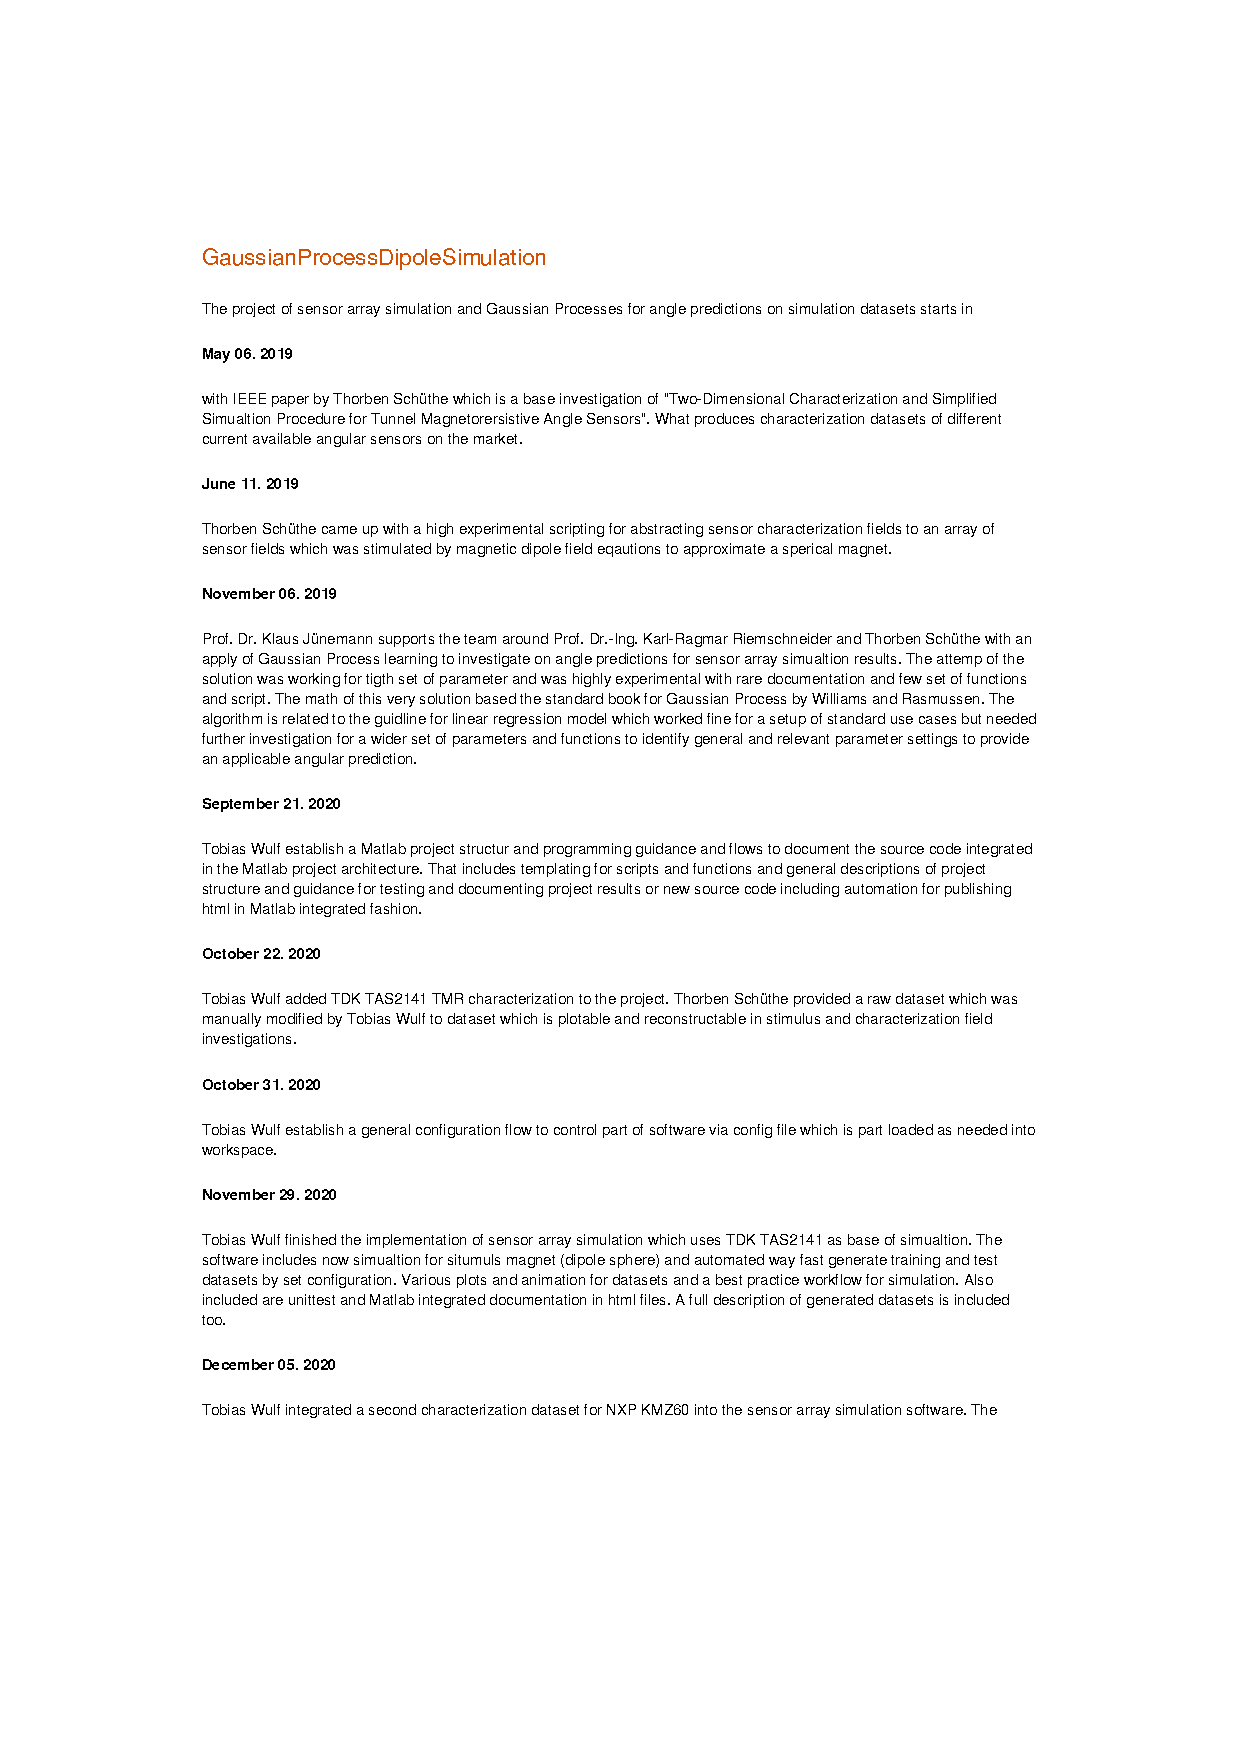
\includepdf[page=1,pagecommand={\phantomsection\addcontentsline{toc}{section}{\protect\numberline{\thesection}GaussianProcessDipoleSimulation}\label{GaussianProcessDipoleSimulation}}]{GaussianProcessDipoleSimulation.pdf}
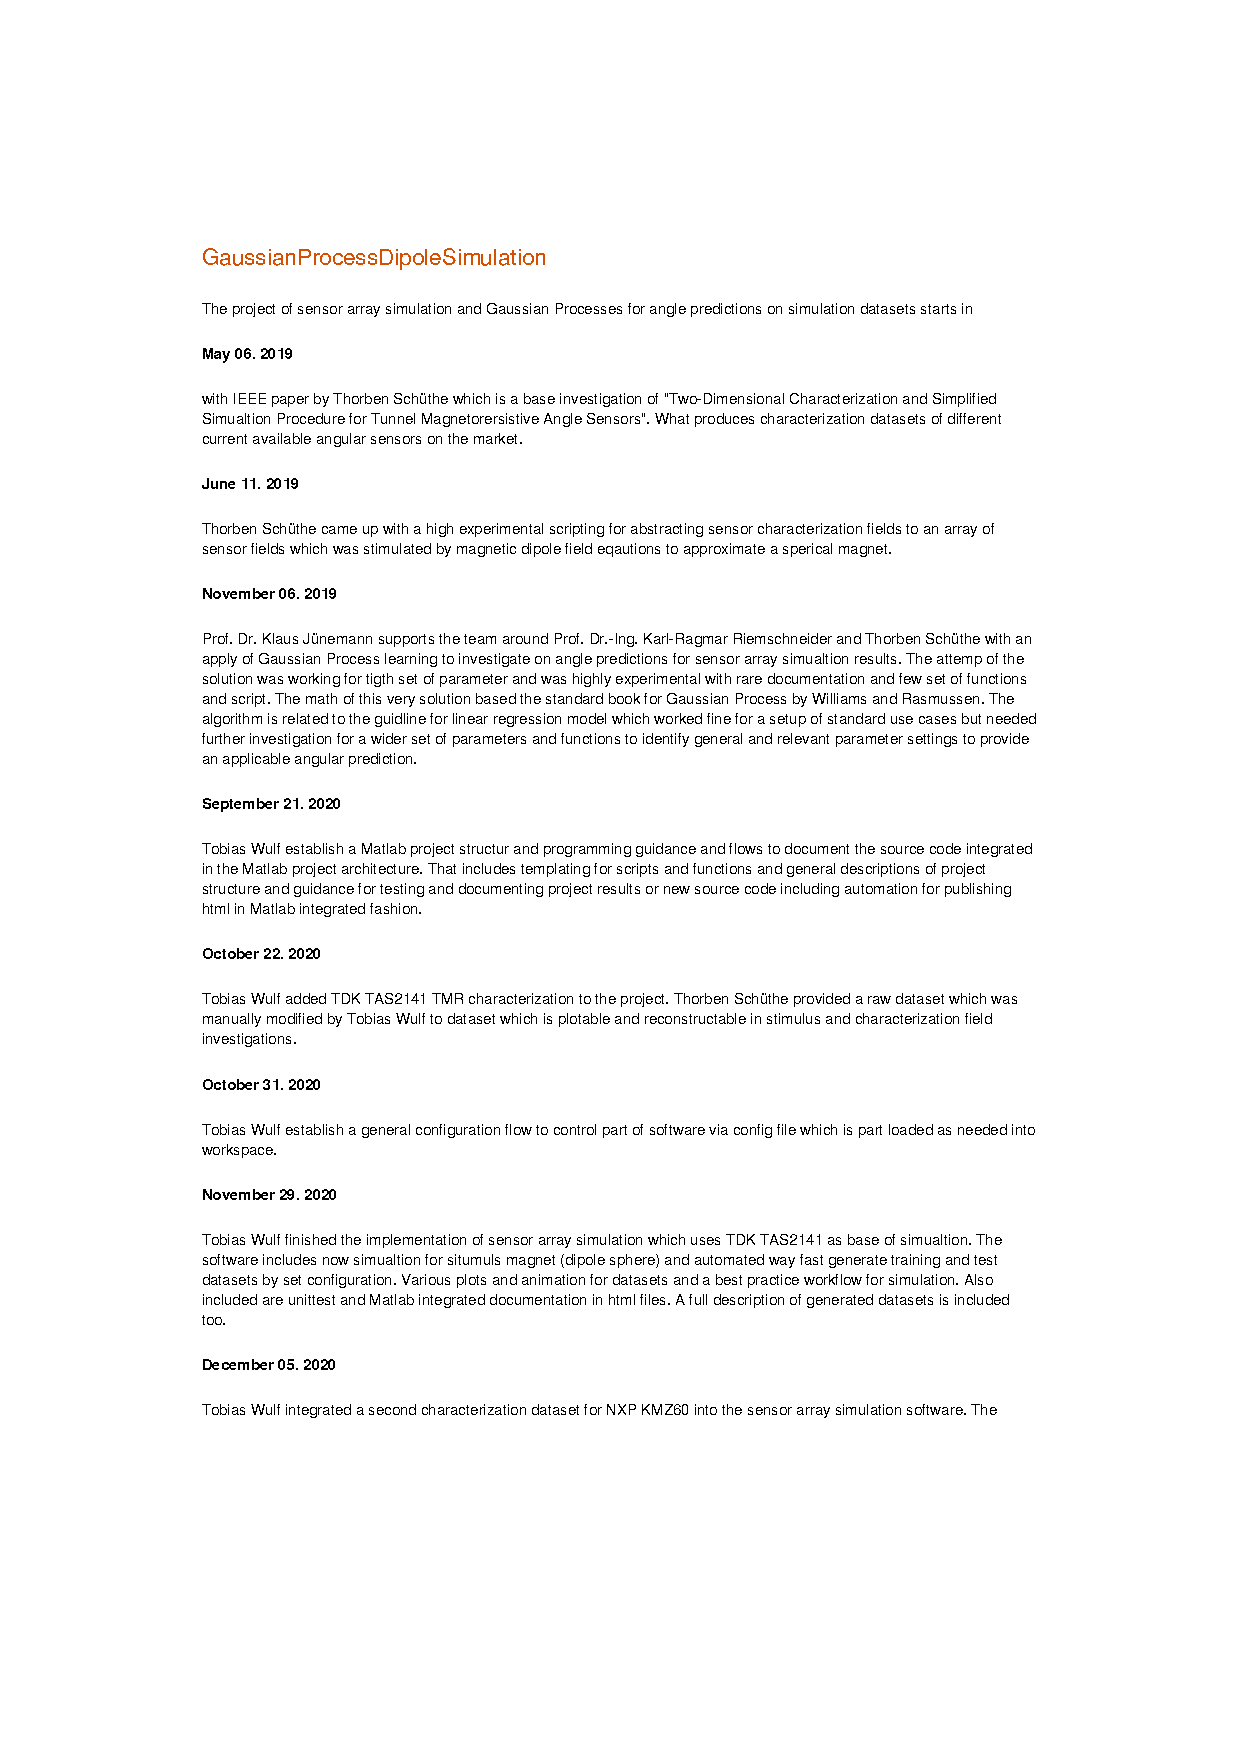
\includepdf[page=2-, pagecommand={\phantomsection}]{GaussianProcessDipoleSimulation.pdf}
\addtocounter{section}{1}
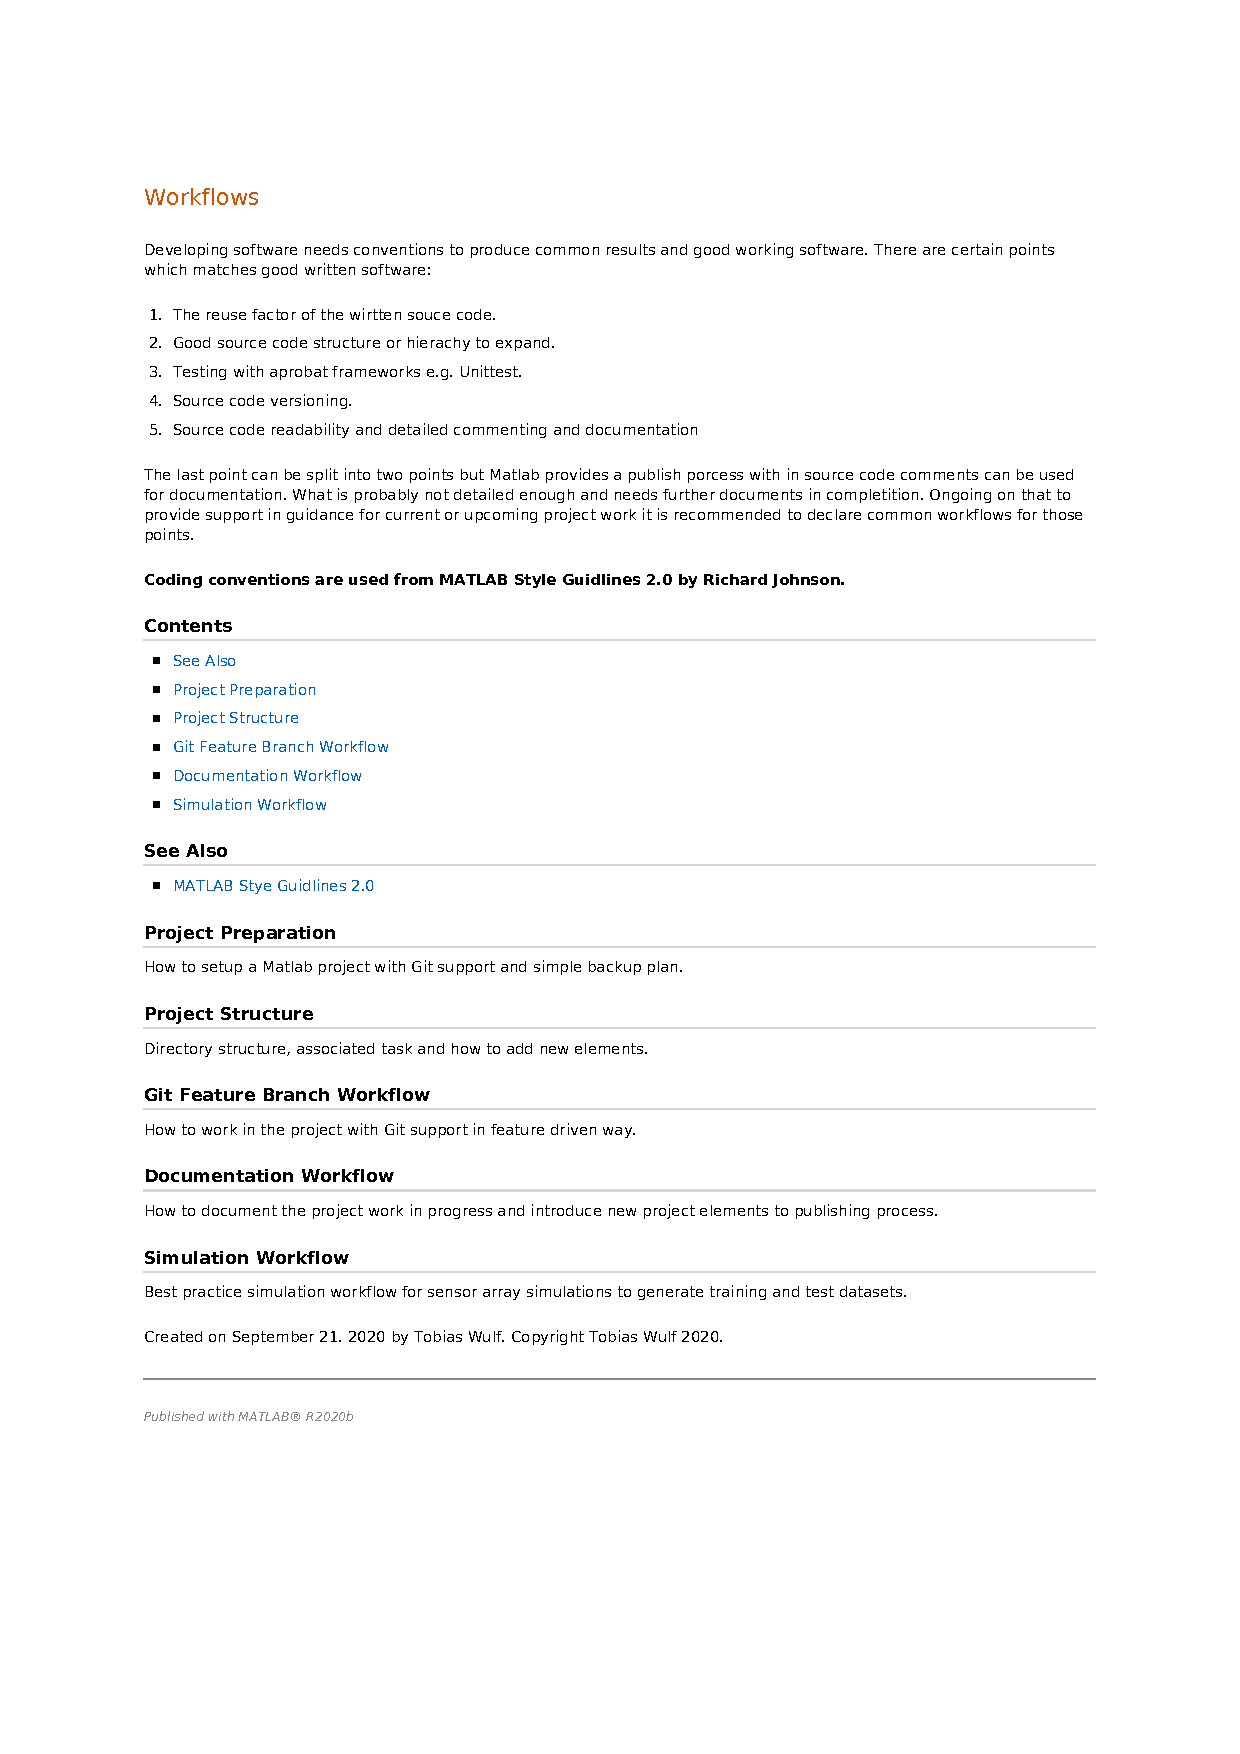
\includepdf[page=1,pagecommand={\phantomsection\addcontentsline{toc}{section}{\protect\numberline{\thesection}Workflows}\label{Workflows}}]{Workflows.pdf}
\addtocounter{subsection}{1}
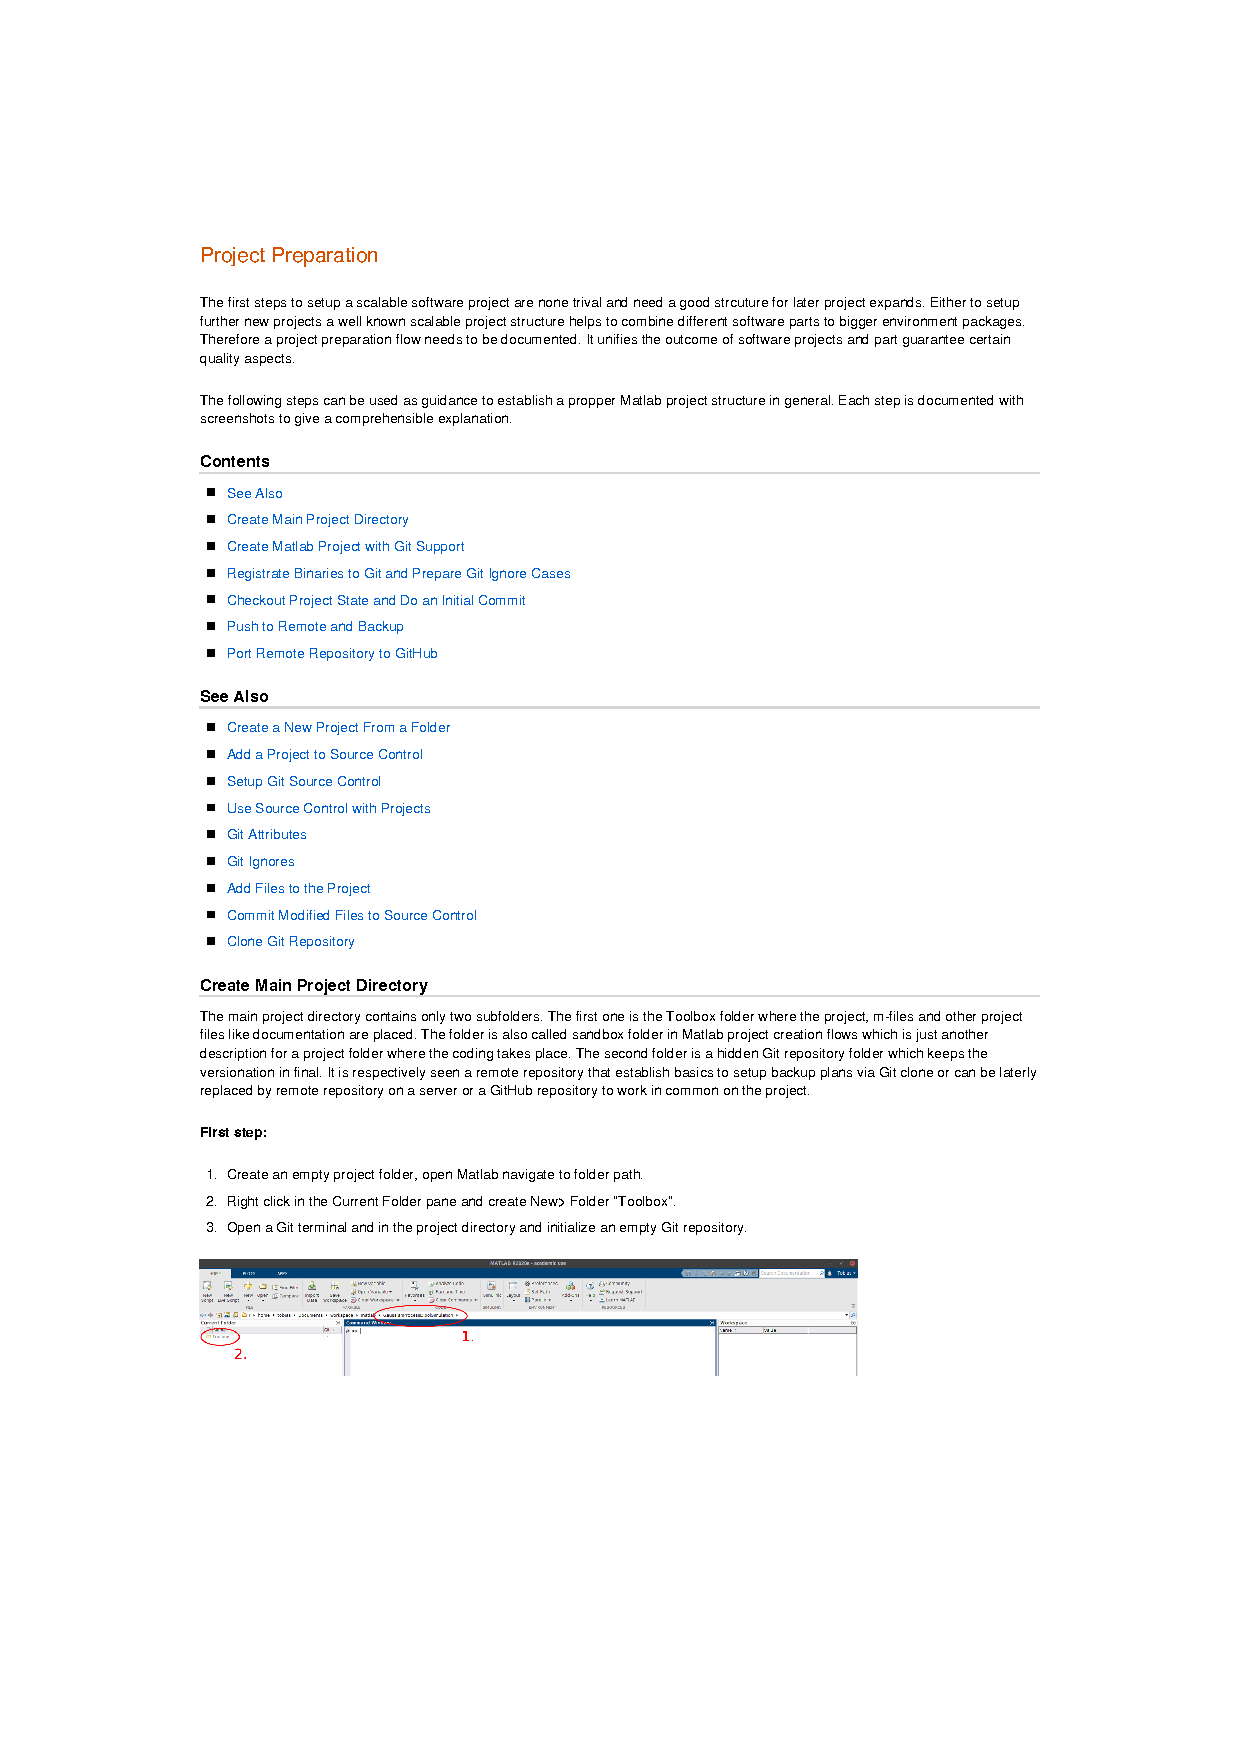
\includepdf[page=1,pagecommand={\phantomsection\addcontentsline{toc}{subsection}{\protect\numberline{\thesubsection}Project Preparation}\label{Project Preparation}}]{Project_Preparation.pdf}
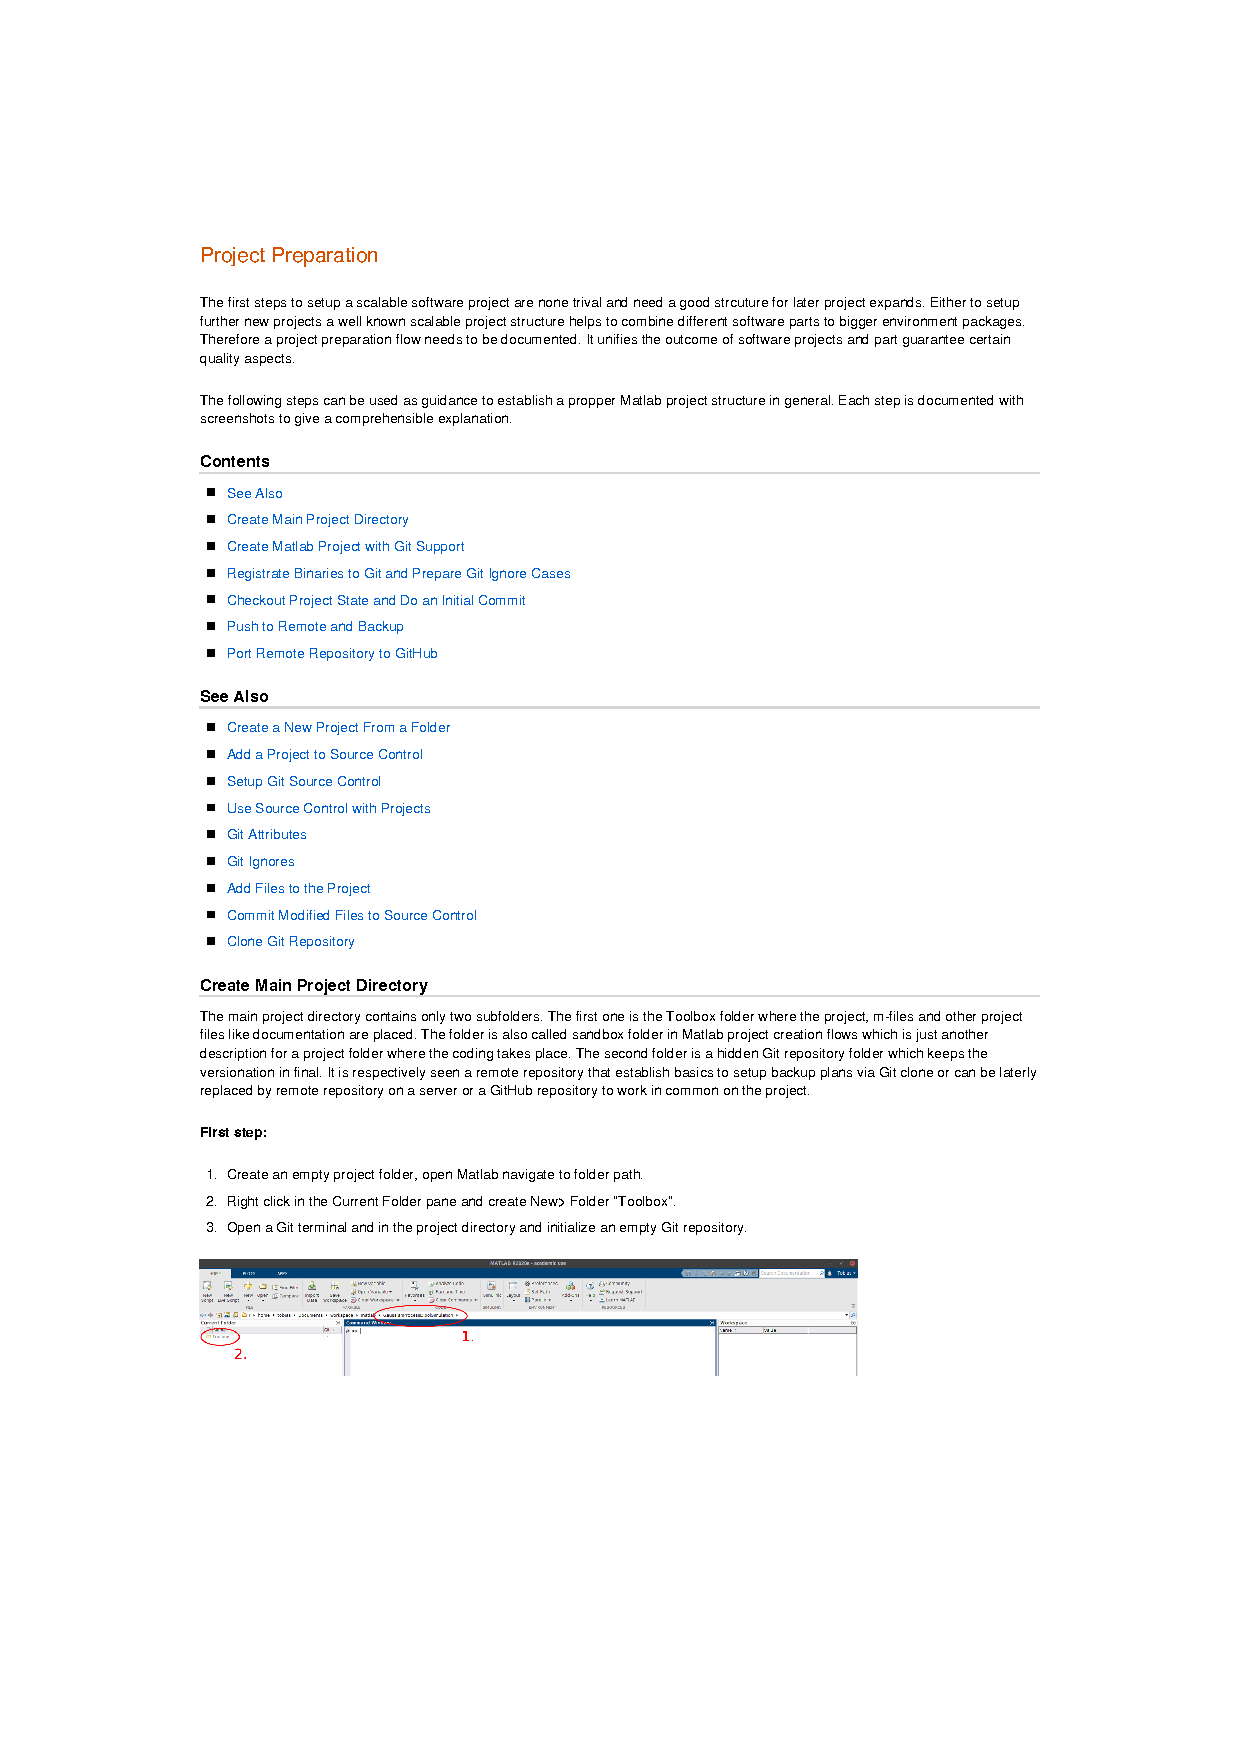
\includepdf[page=2-, pagecommand={\phantomsection}]{Project_Preparation.pdf}
\addtocounter{subsection}{1}
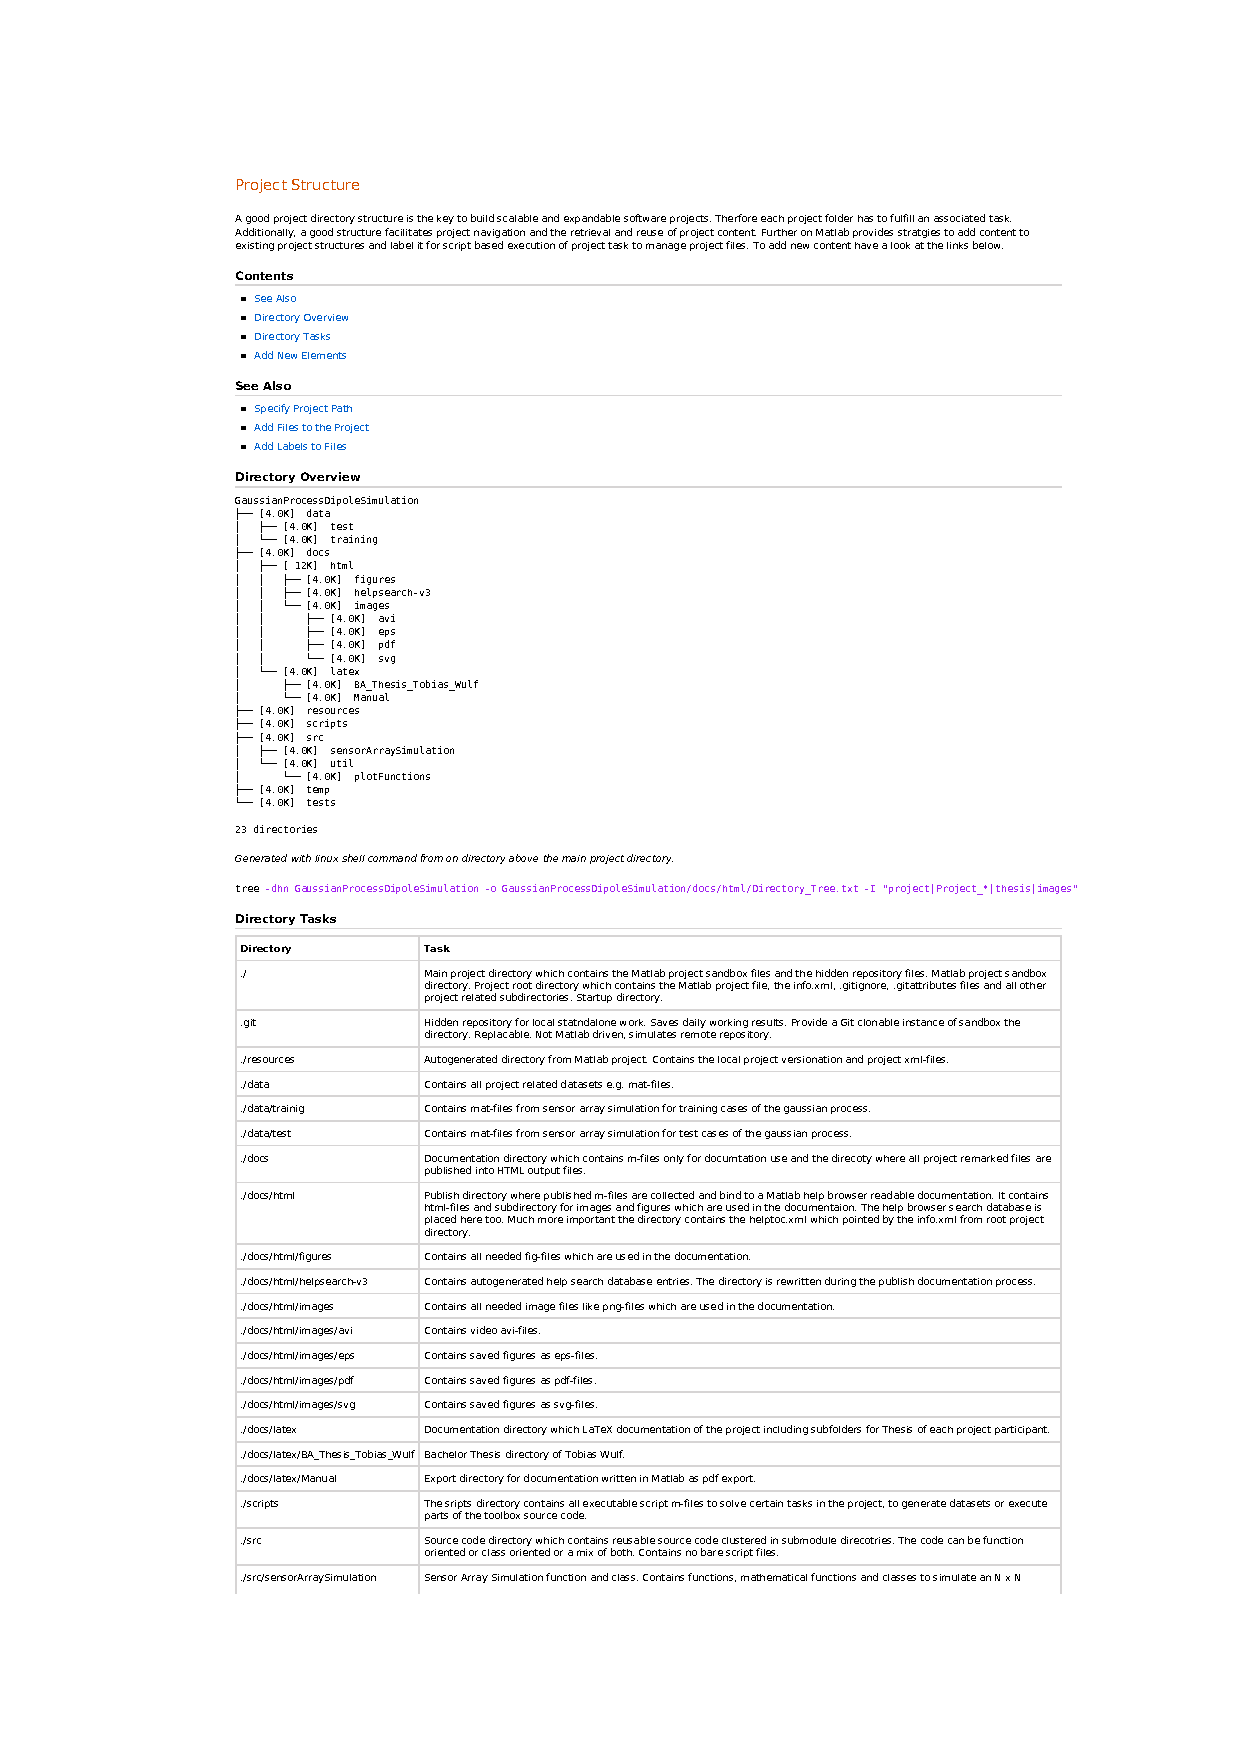
\includepdf[page=1,pagecommand={\phantomsection\addcontentsline{toc}{subsection}{\protect\numberline{\thesubsection}Project Structure}\label{Project Structure}}]{Project_Structure.pdf}
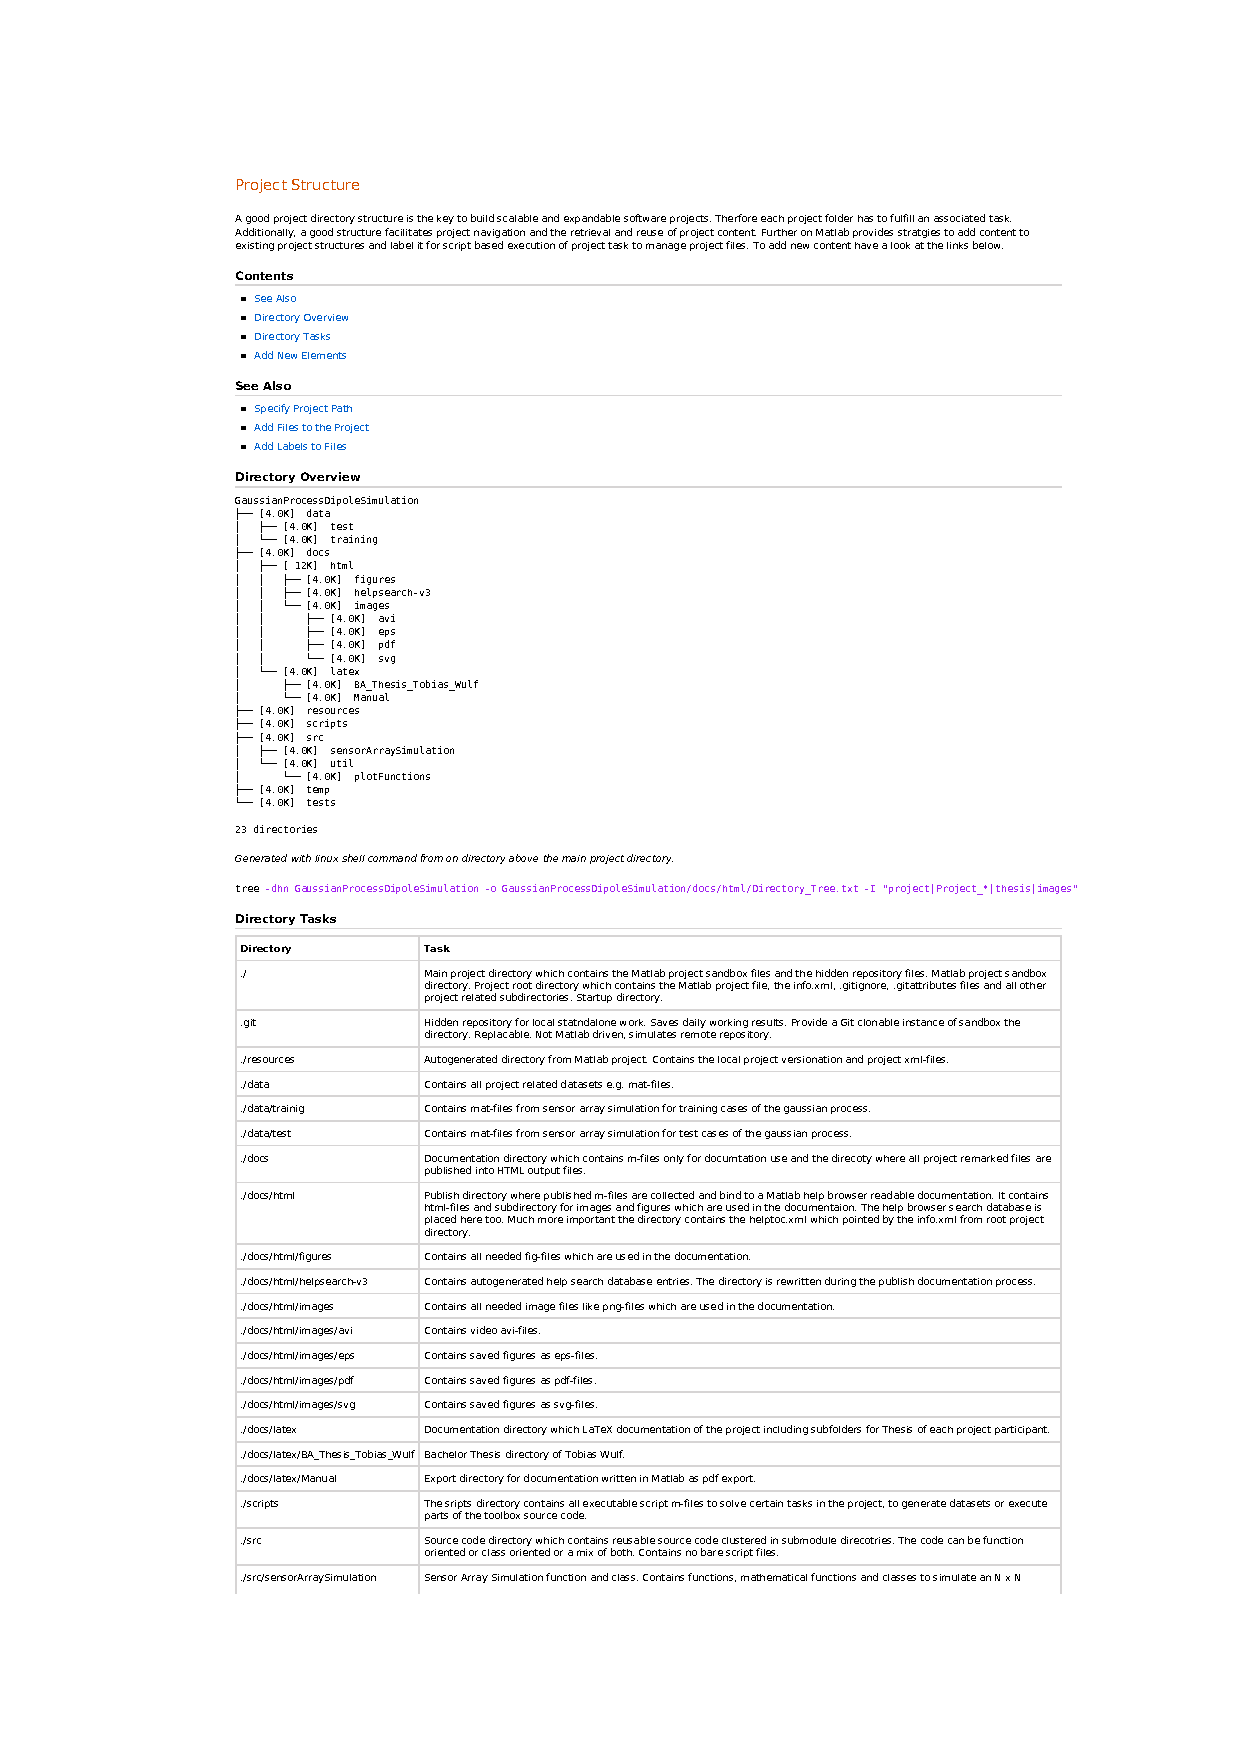
\includepdf[page=2-, pagecommand={\phantomsection}]{Project_Structure.pdf}
\addtocounter{subsection}{1}
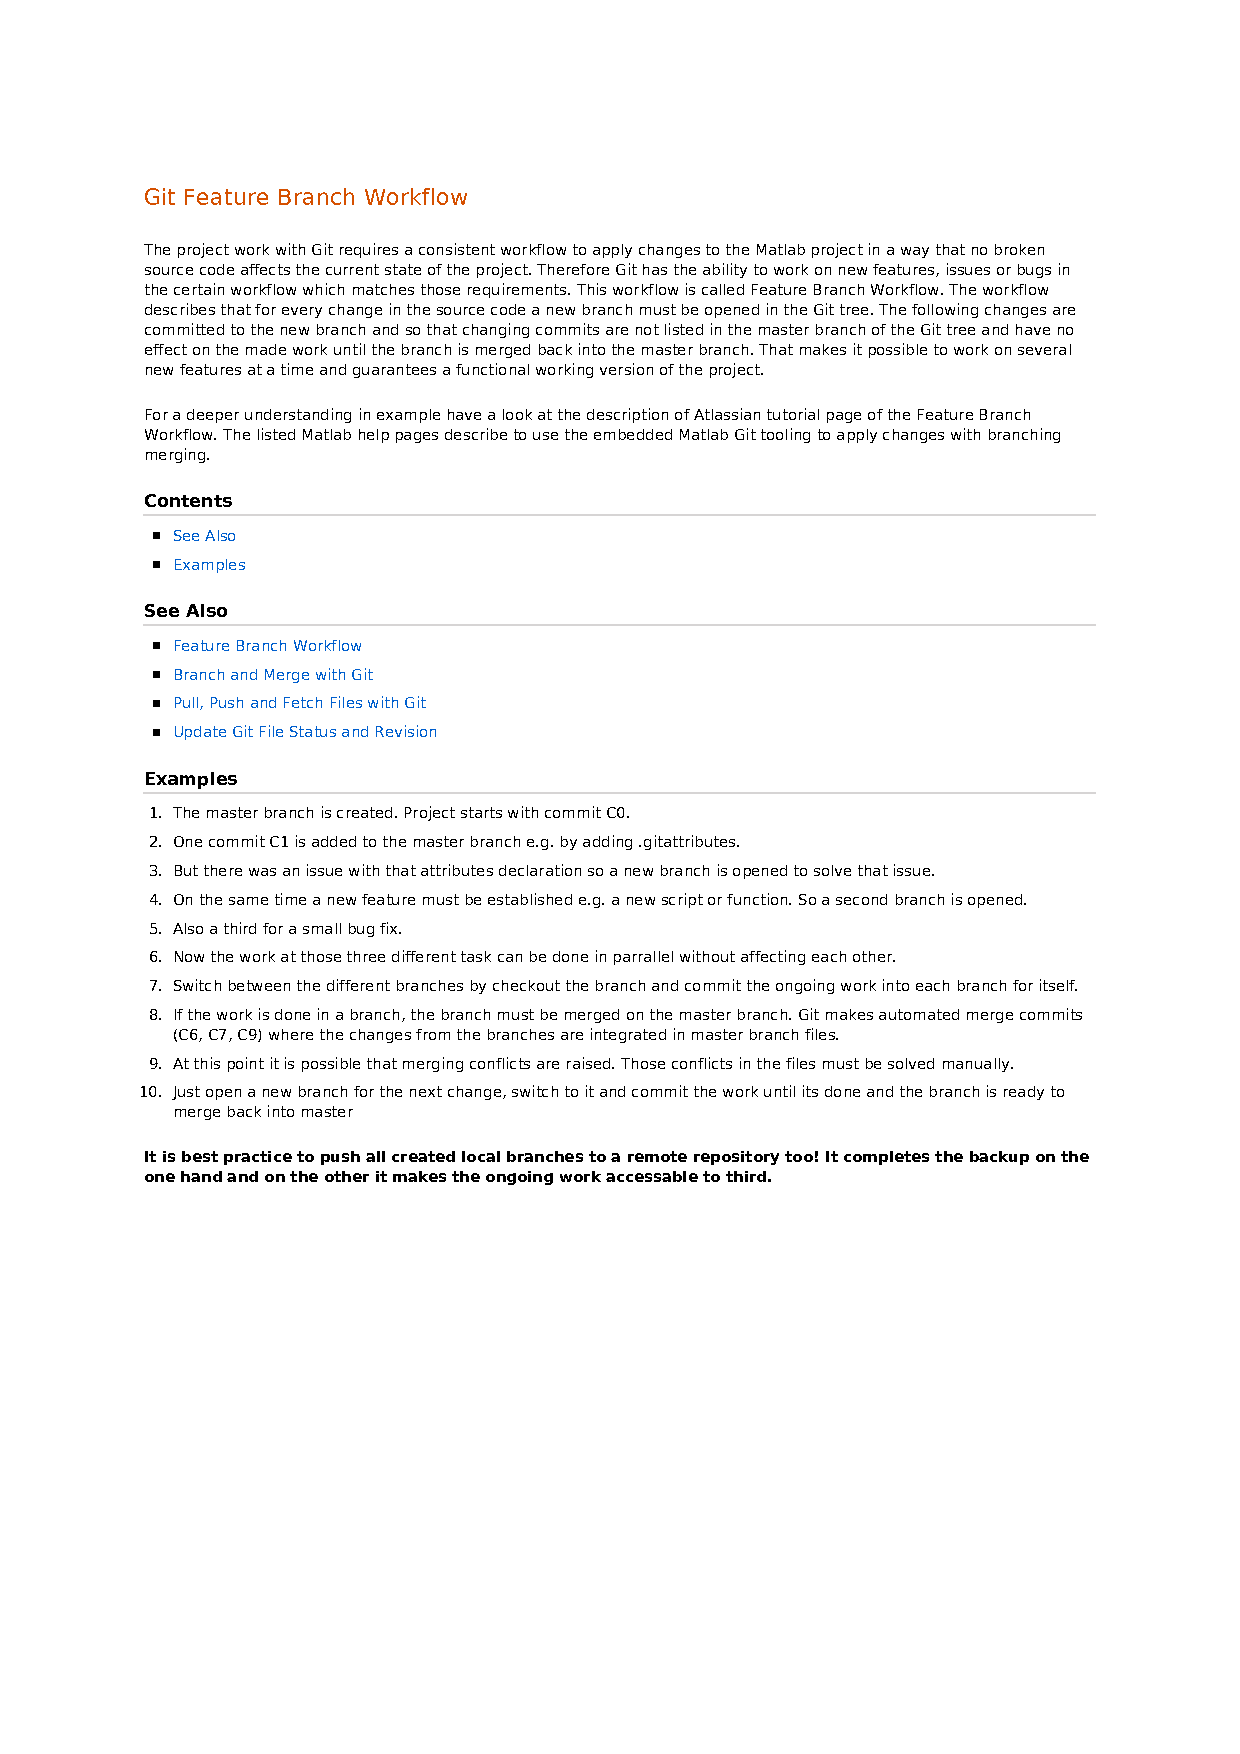
\includepdf[page=1,pagecommand={\phantomsection\addcontentsline{toc}{subsection}{\protect\numberline{\thesubsection}Git Feature Branch Workflow}\label{Git Feature Branch Workflow}}]{Git_Feature_Branch_Workflow.pdf}
\addtocounter{subsection}{1}
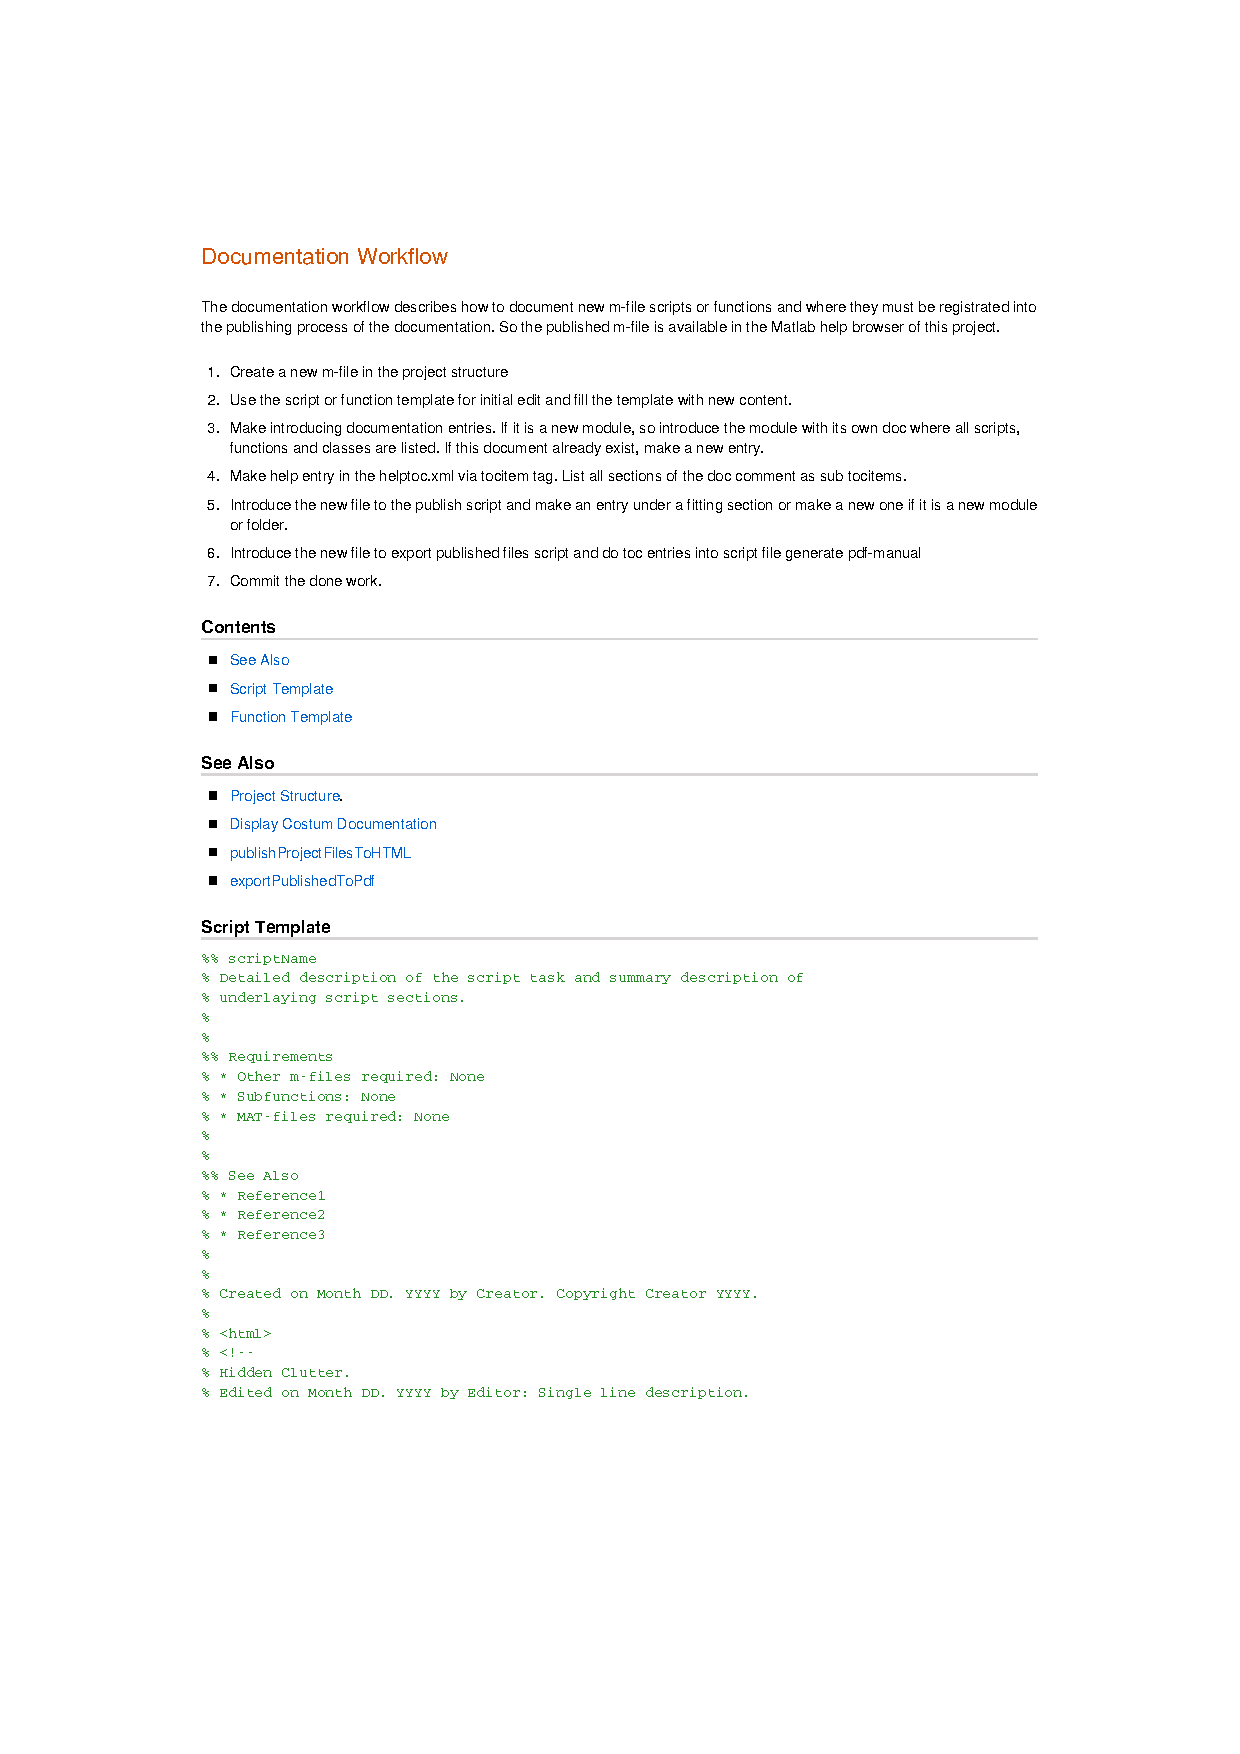
\includepdf[page=1,pagecommand={\phantomsection\addcontentsline{toc}{subsection}{\protect\numberline{\thesubsection}Documentation Workflow}\label{Documentation Workflow}}]{Documentation_Workflow.pdf}
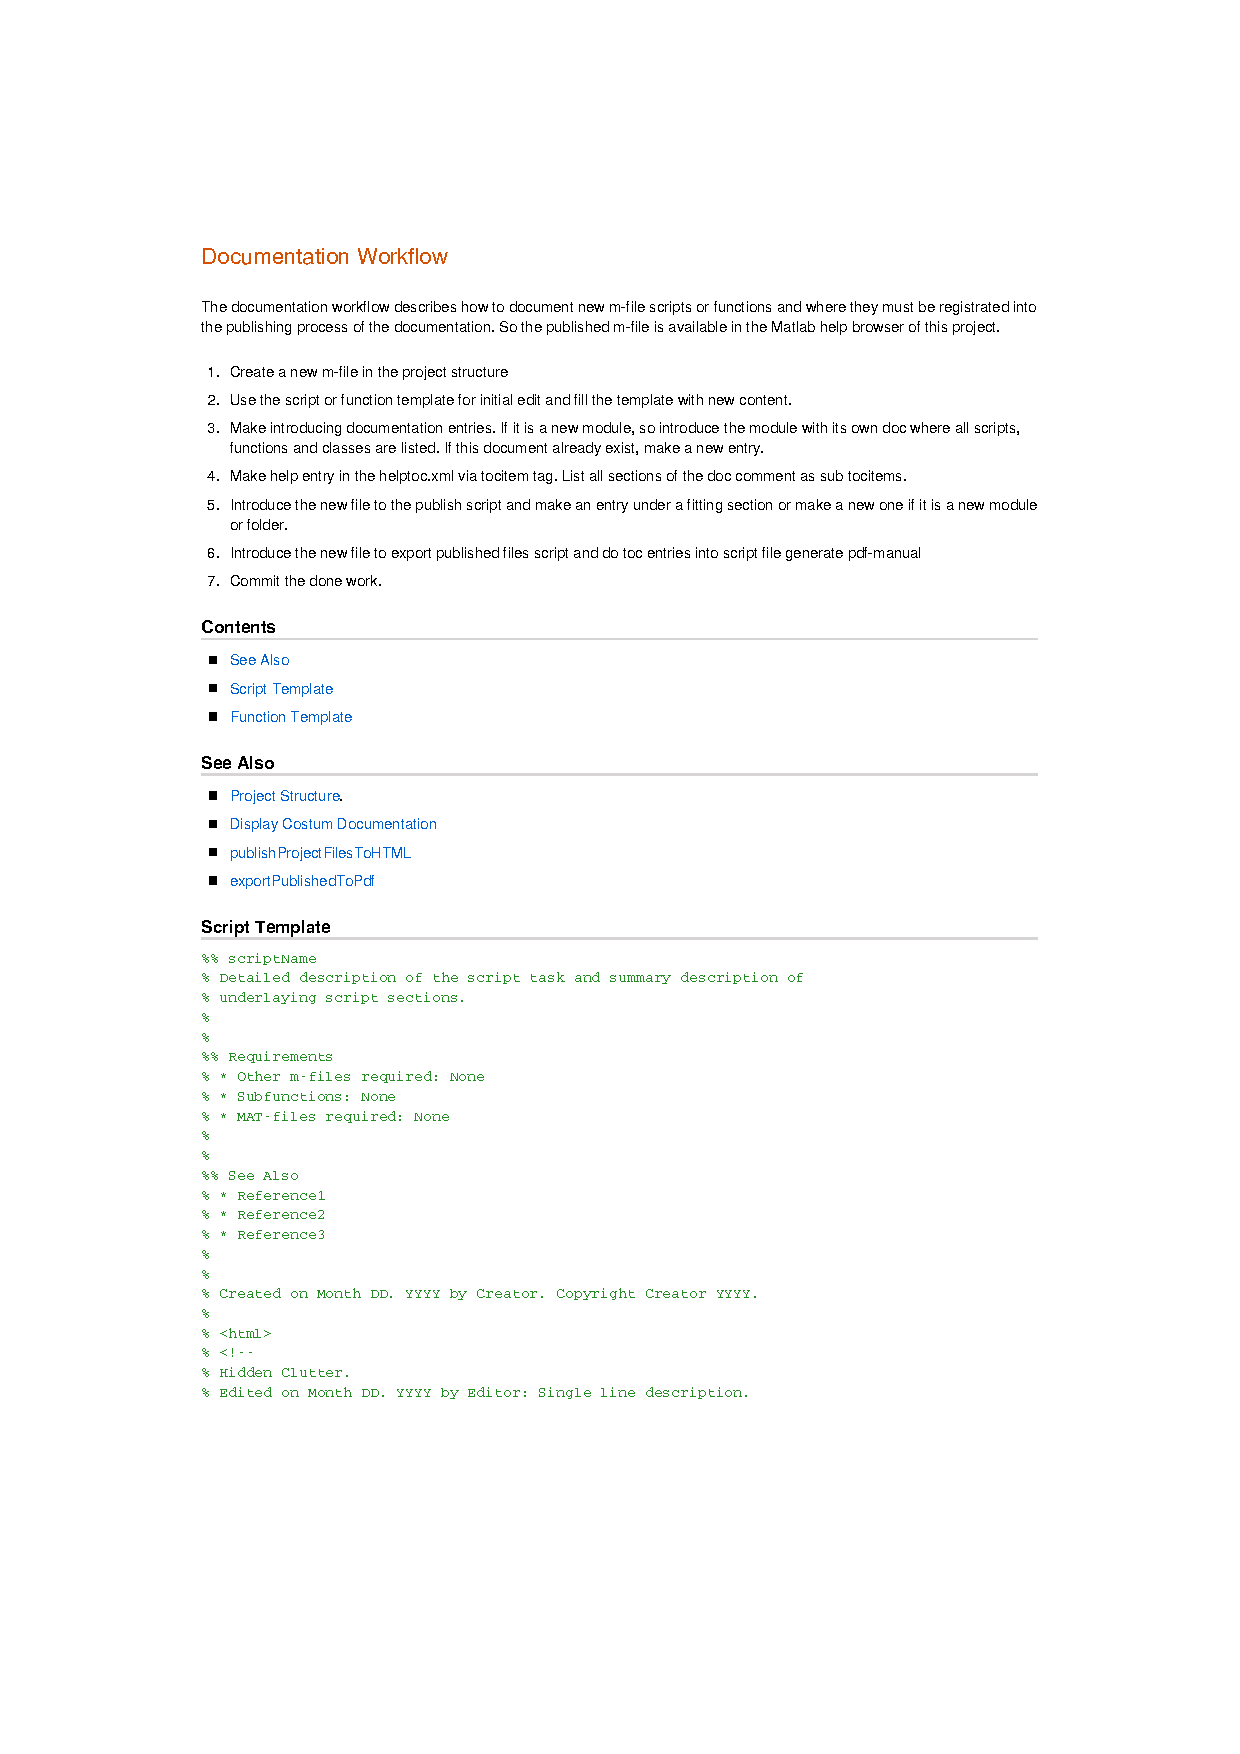
\includepdf[page=2-, pagecommand={\phantomsection}]{Documentation_Workflow.pdf}
\addtocounter{subsection}{1}
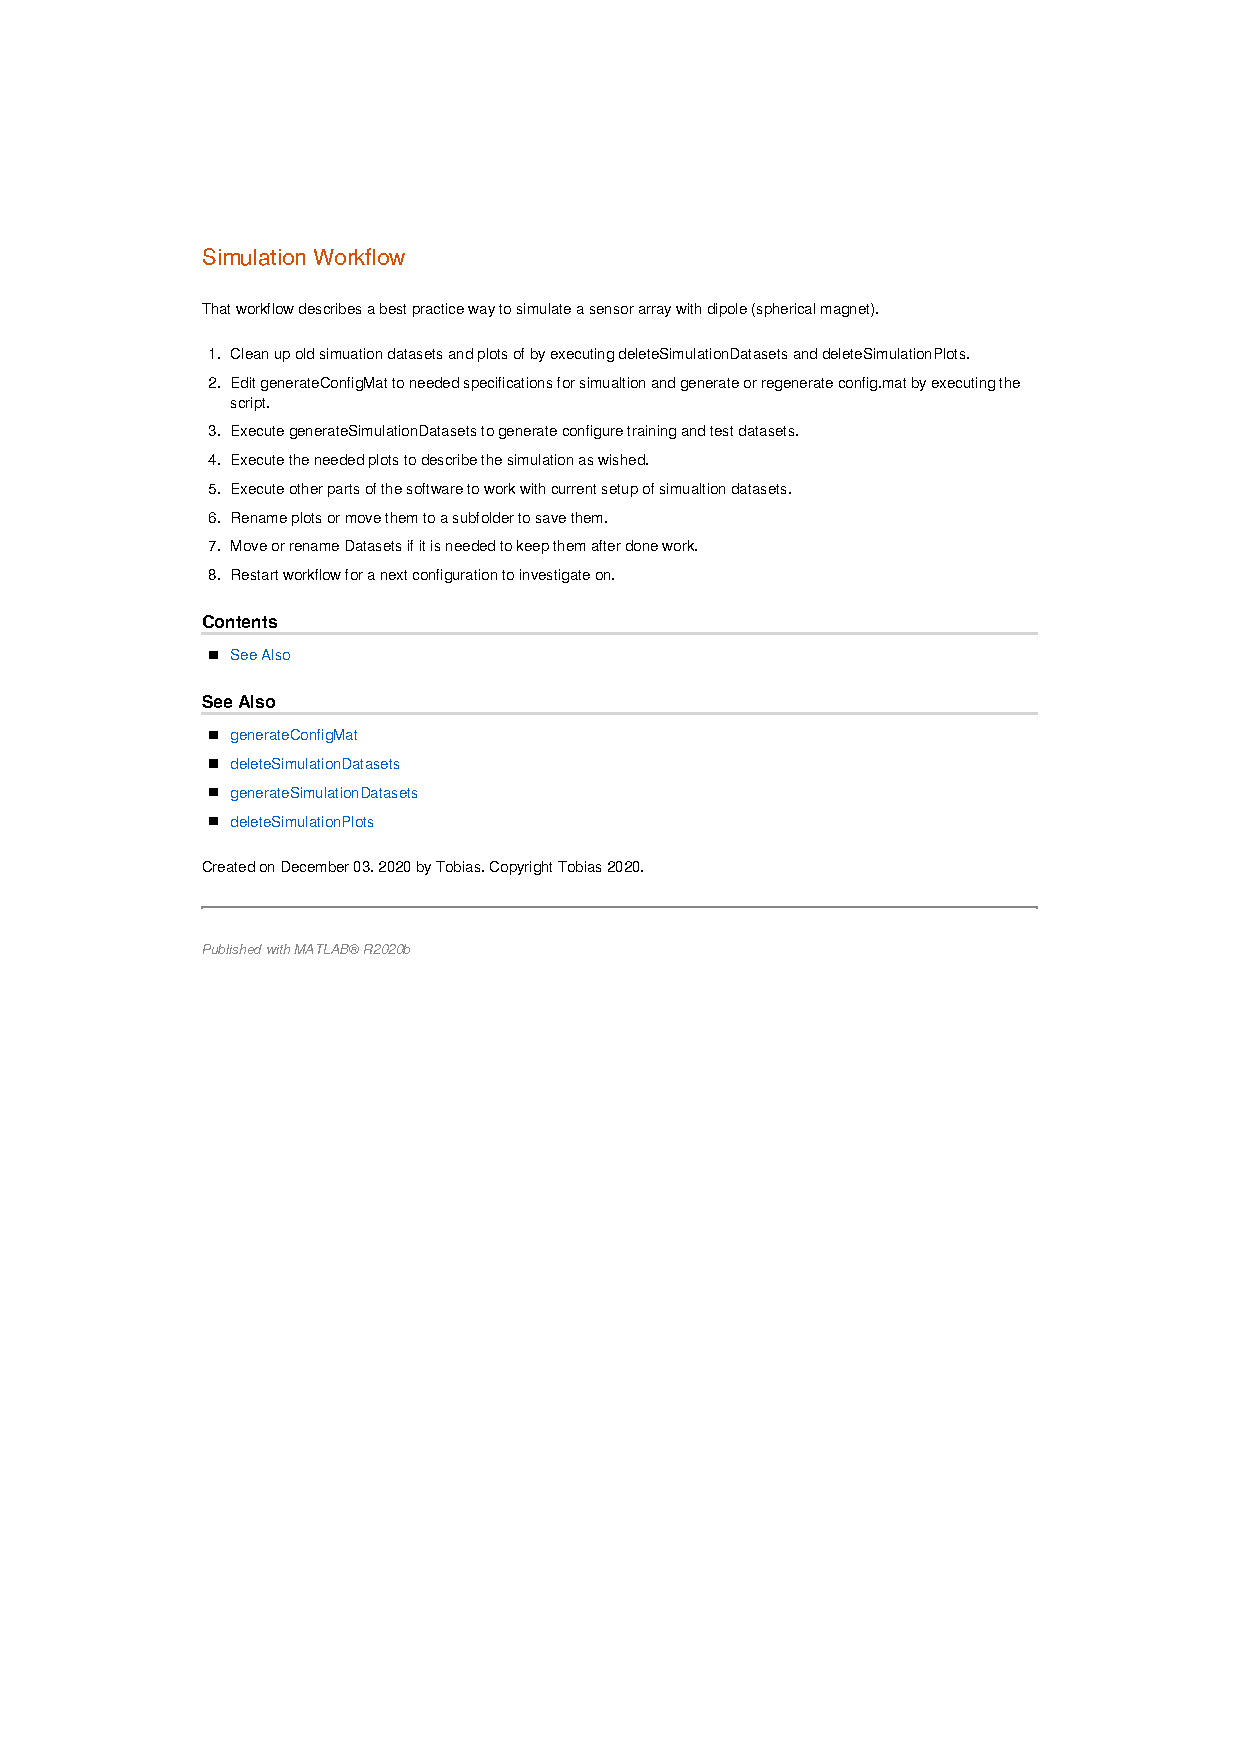
\includepdf[page=1,pagecommand={\phantomsection\addcontentsline{toc}{subsection}{\protect\numberline{\thesubsection}Simulation Workflow}\label{Simulation Workflow}}]{Simulation_Workflow.pdf}
\addtocounter{section}{1}
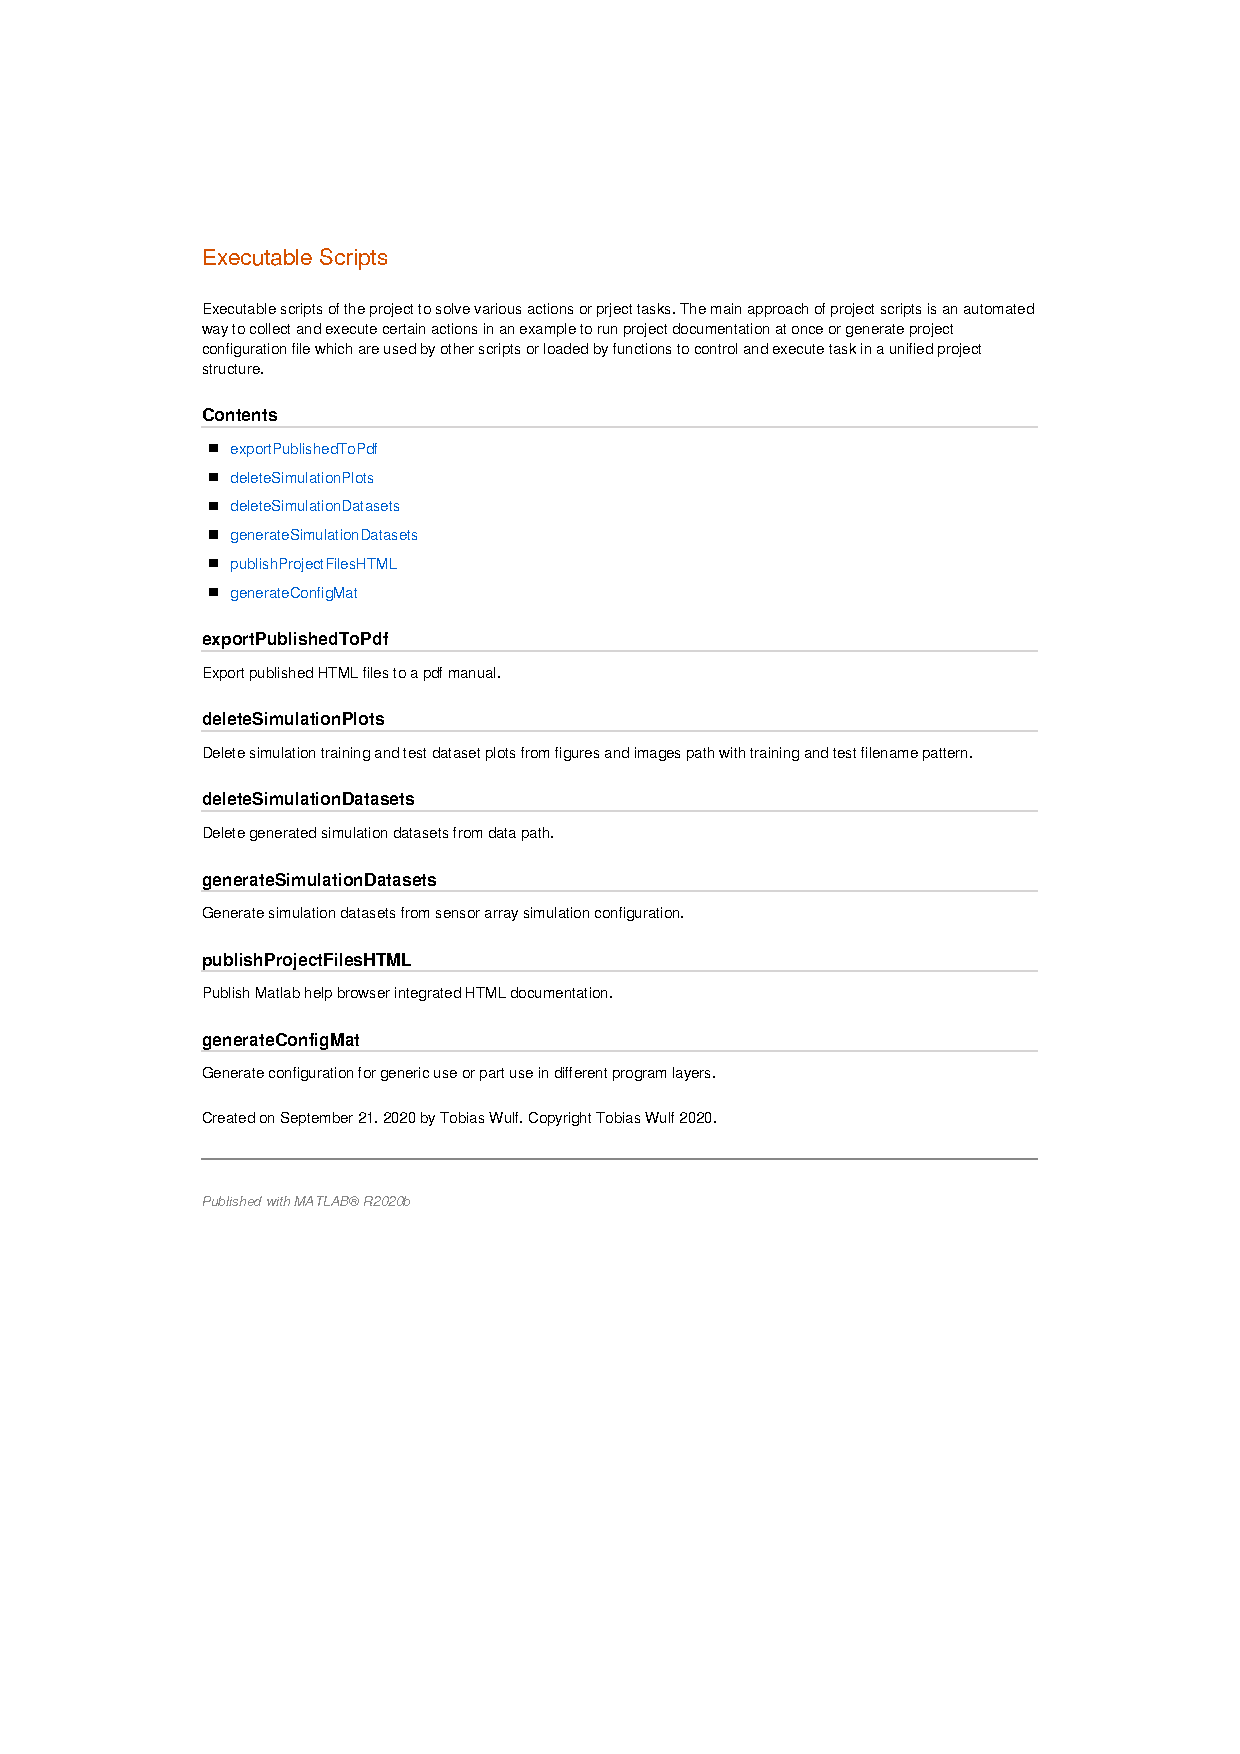
\includepdf[page=1,pagecommand={\phantomsection\addcontentsline{toc}{section}{\protect\numberline{\thesection}Executable Scripts}\label{Executable Scripts}}]{Executable_Scripts.pdf}
\addtocounter{subsection}{1}
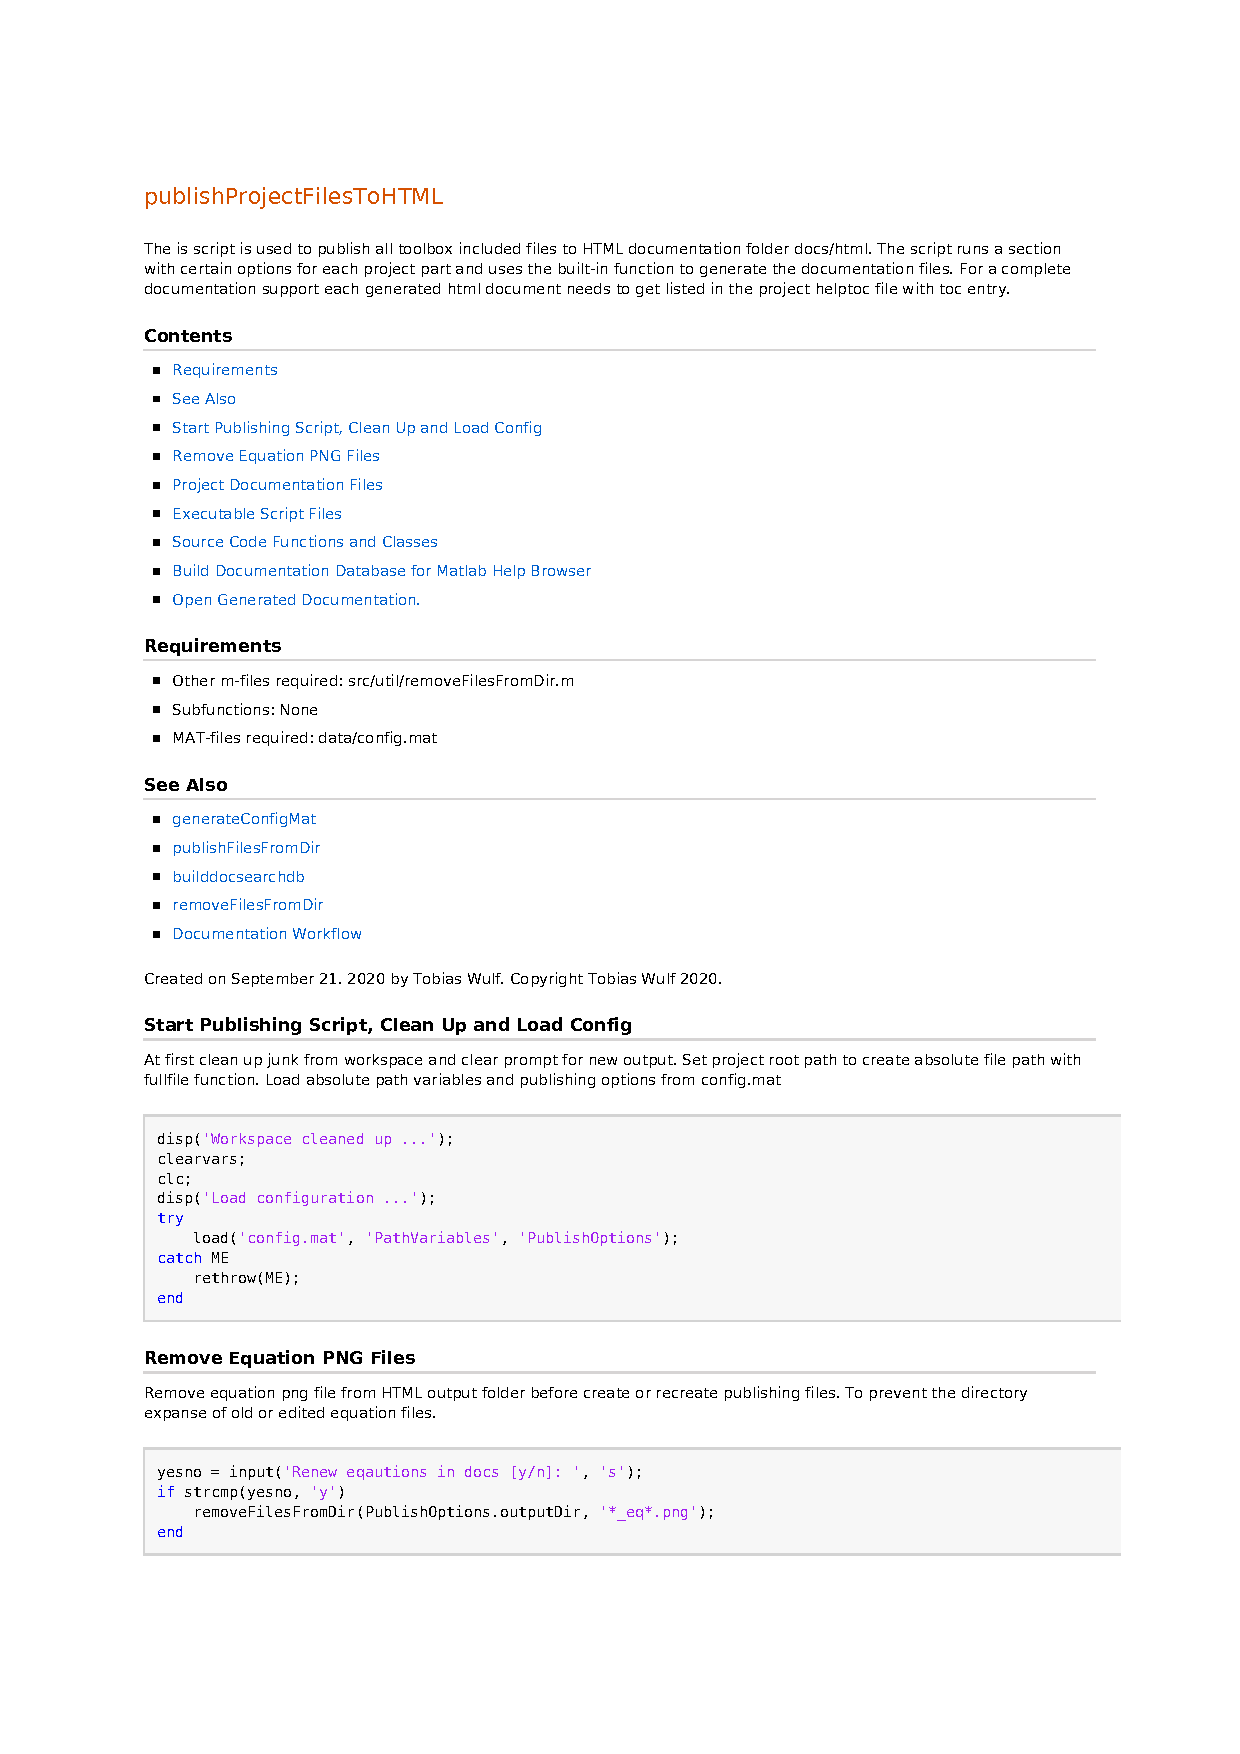
\includepdf[page=1,pagecommand={\phantomsection\addcontentsline{toc}{subsection}{\protect\numberline{\thesubsection}publishProjectFilesToHTML}\label{publishProjectFilesToHTML}}]{publishProjectFilesToHTML.pdf}
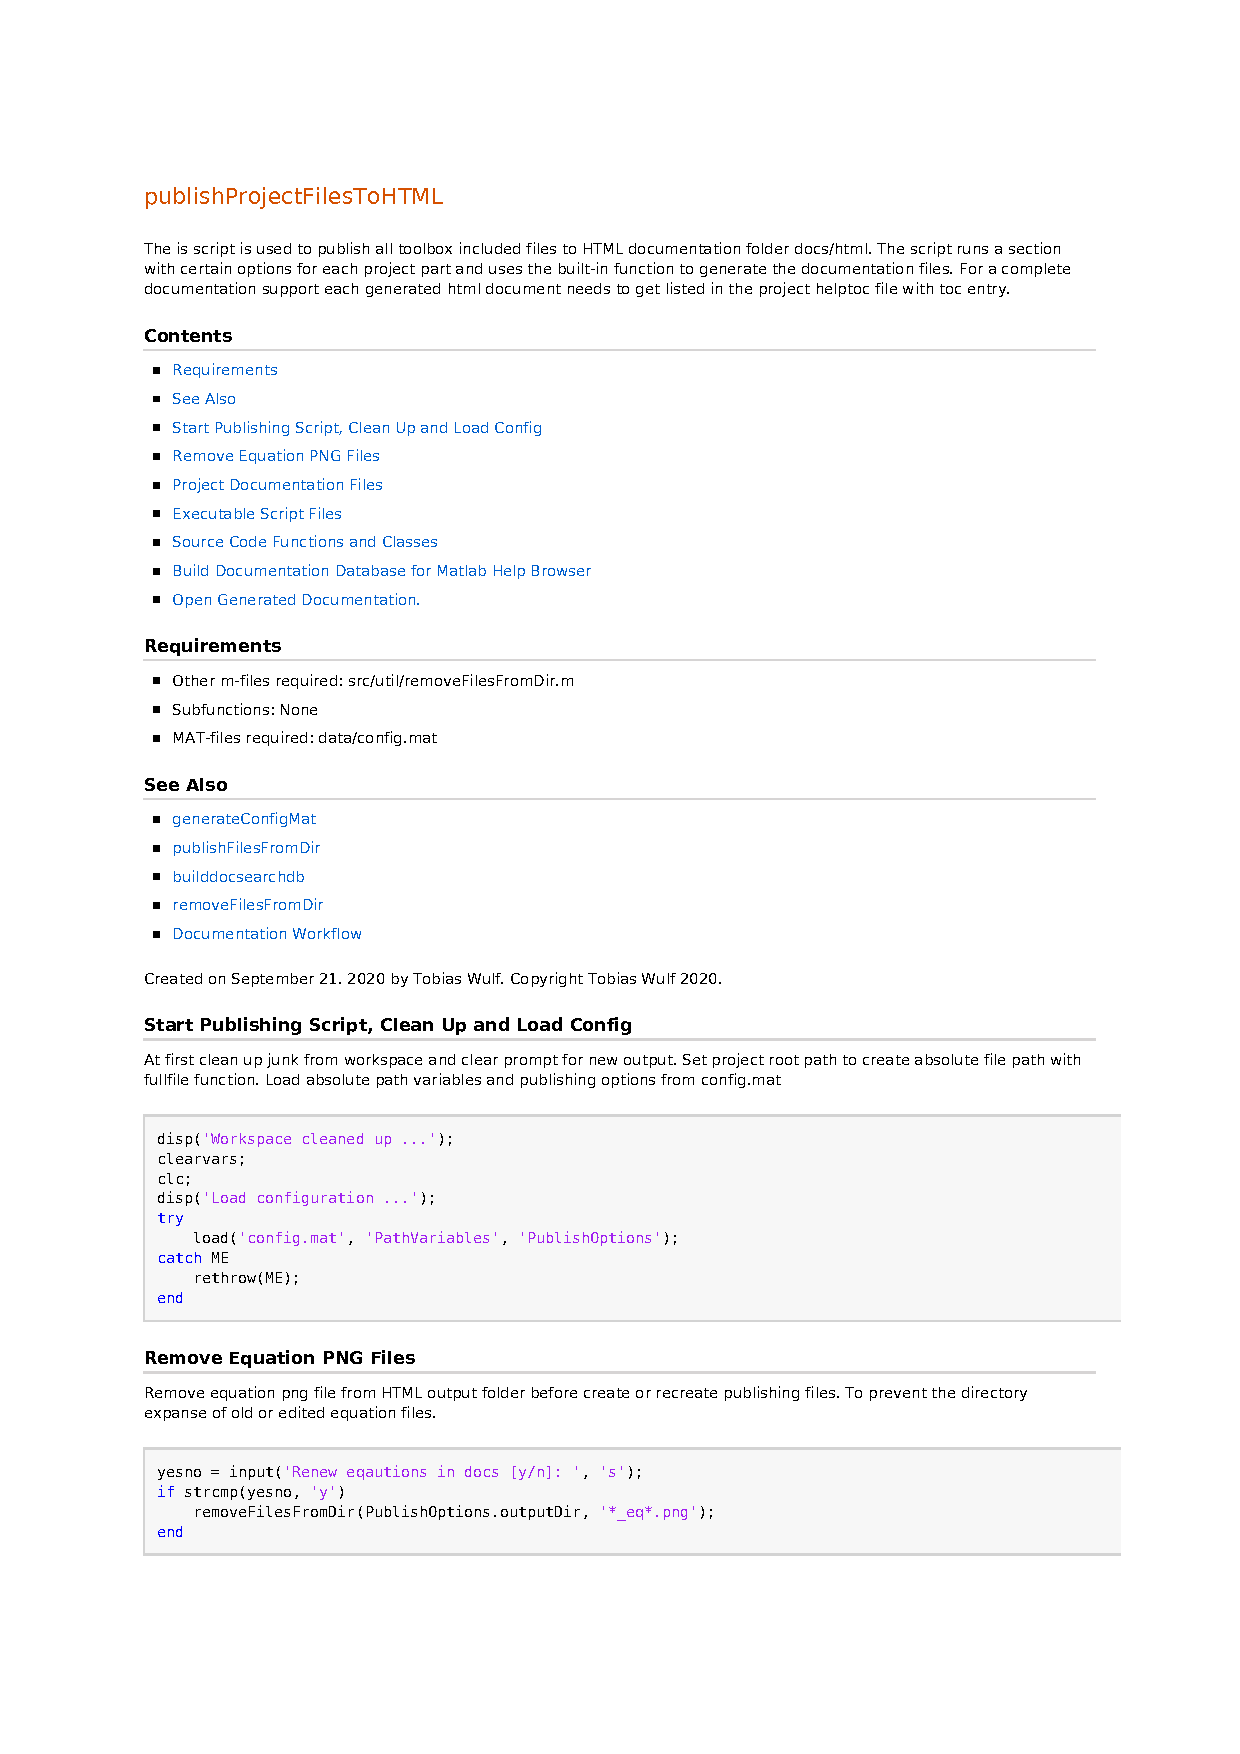
\includepdf[page=2-, pagecommand={\phantomsection}]{publishProjectFilesToHTML.pdf}
\addtocounter{subsection}{1}
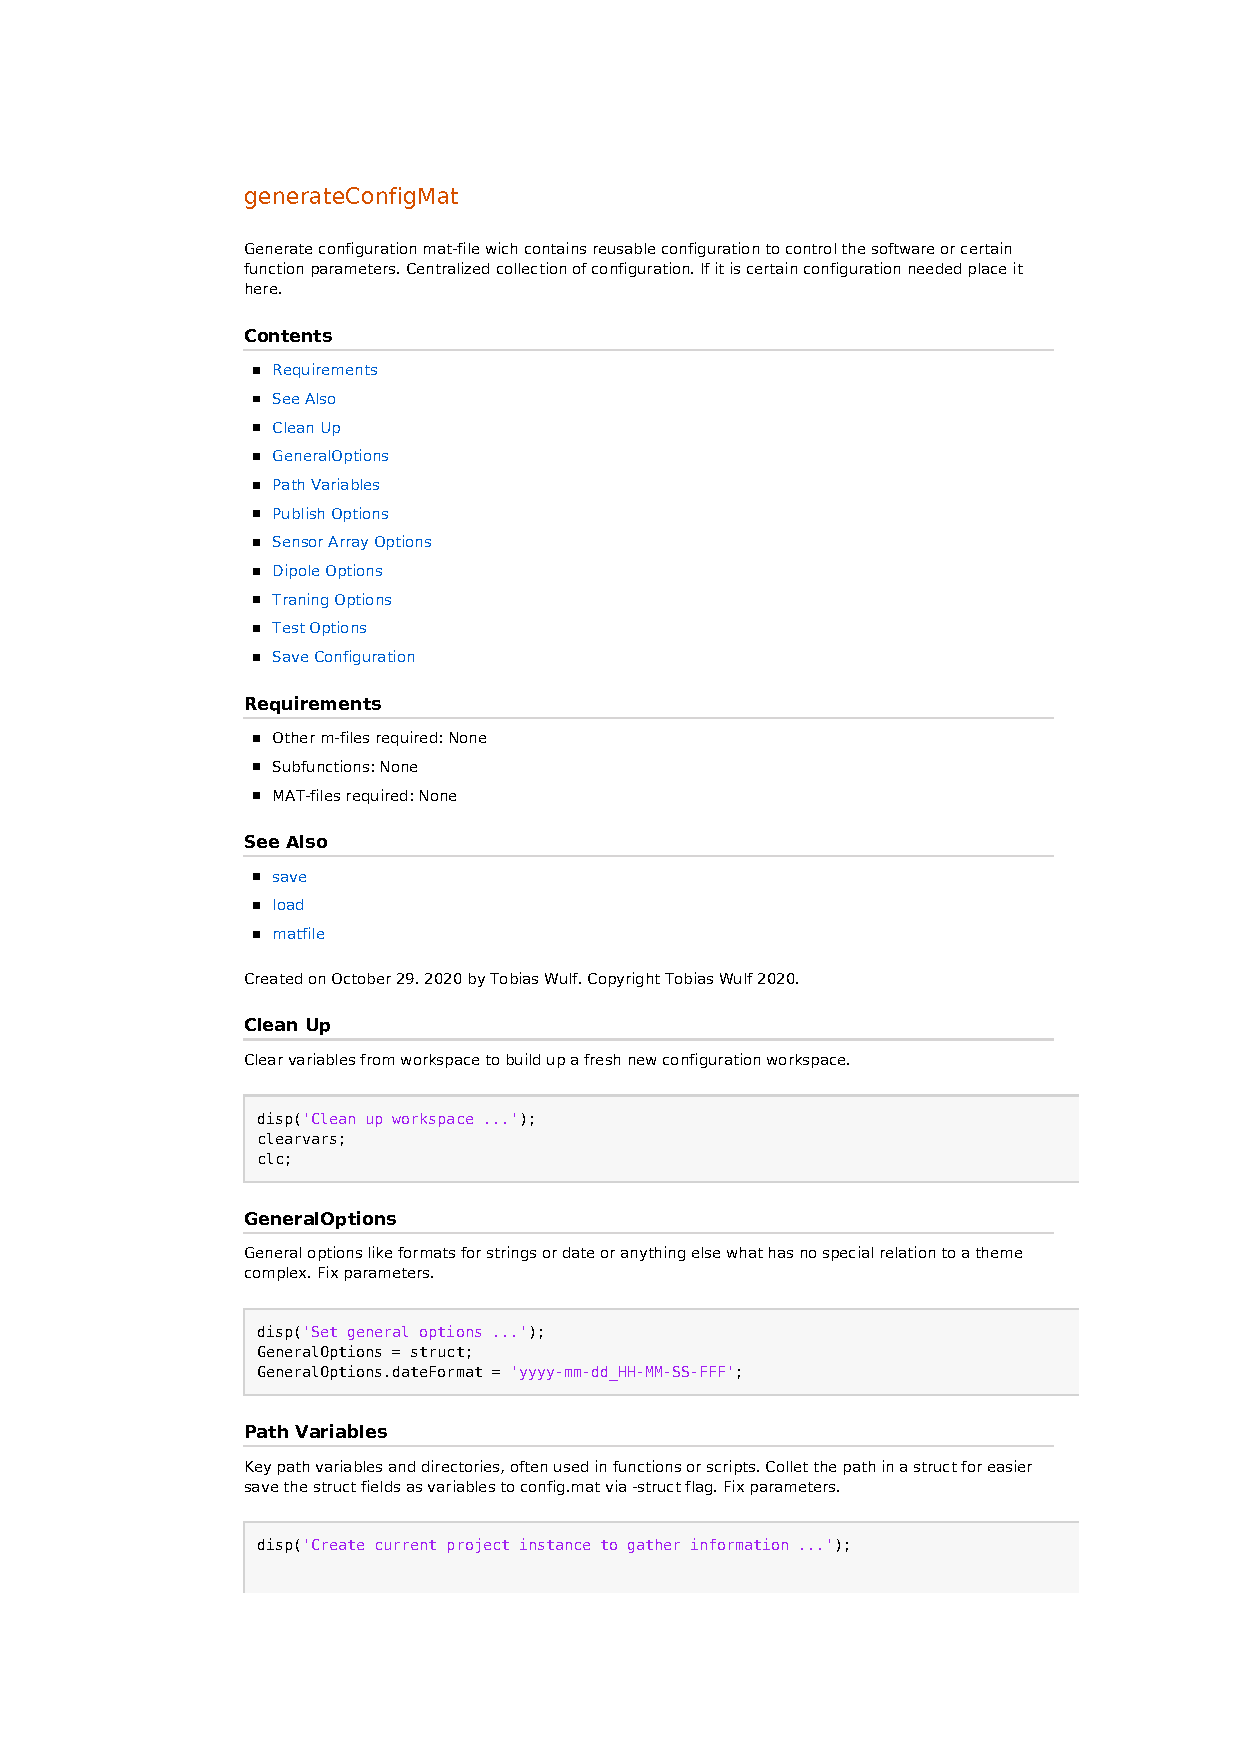
\includepdf[page=1,pagecommand={\phantomsection\addcontentsline{toc}{subsection}{\protect\numberline{\thesubsection}generateConfigMat}\label{generateConfigMat}}]{generateConfigMat.pdf}
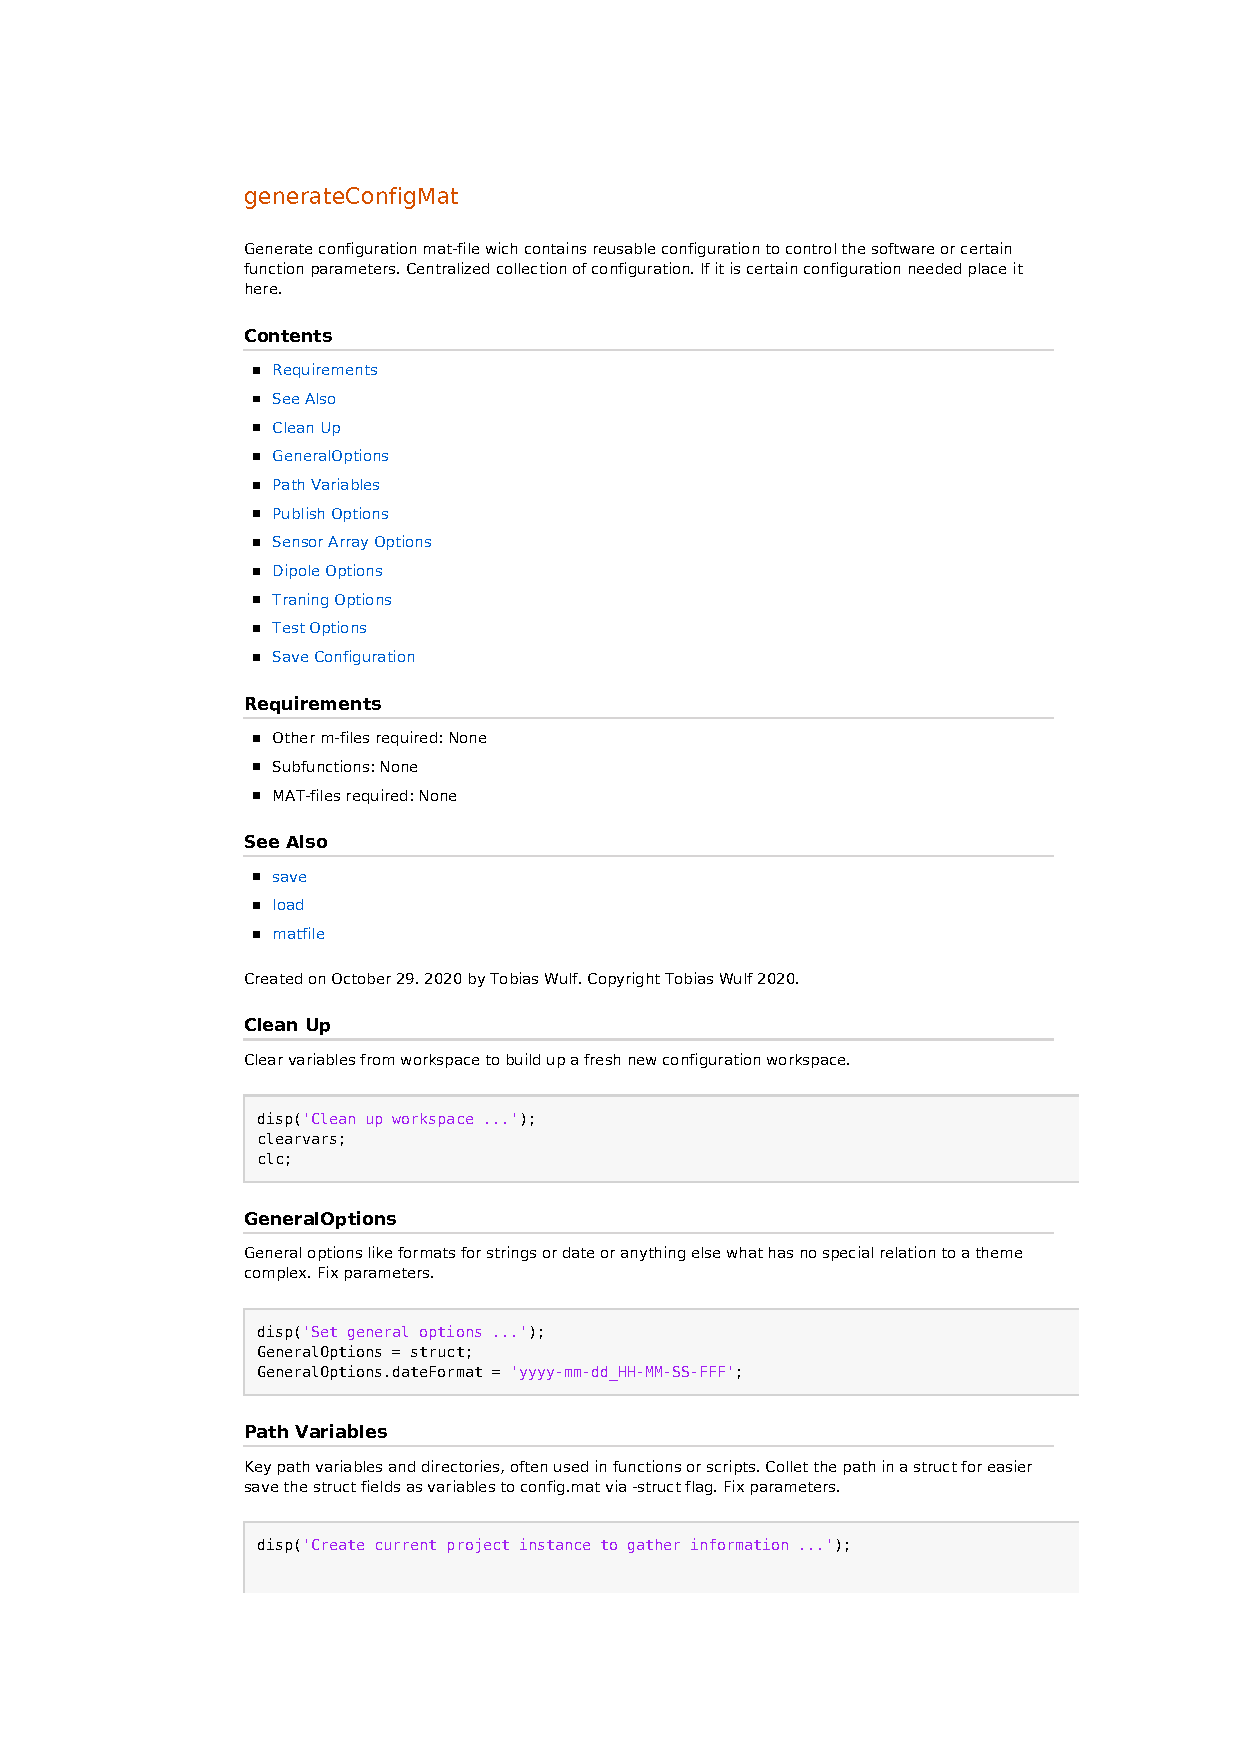
\includepdf[page=2-, pagecommand={\phantomsection}]{generateConfigMat.pdf}
\addtocounter{subsection}{1}
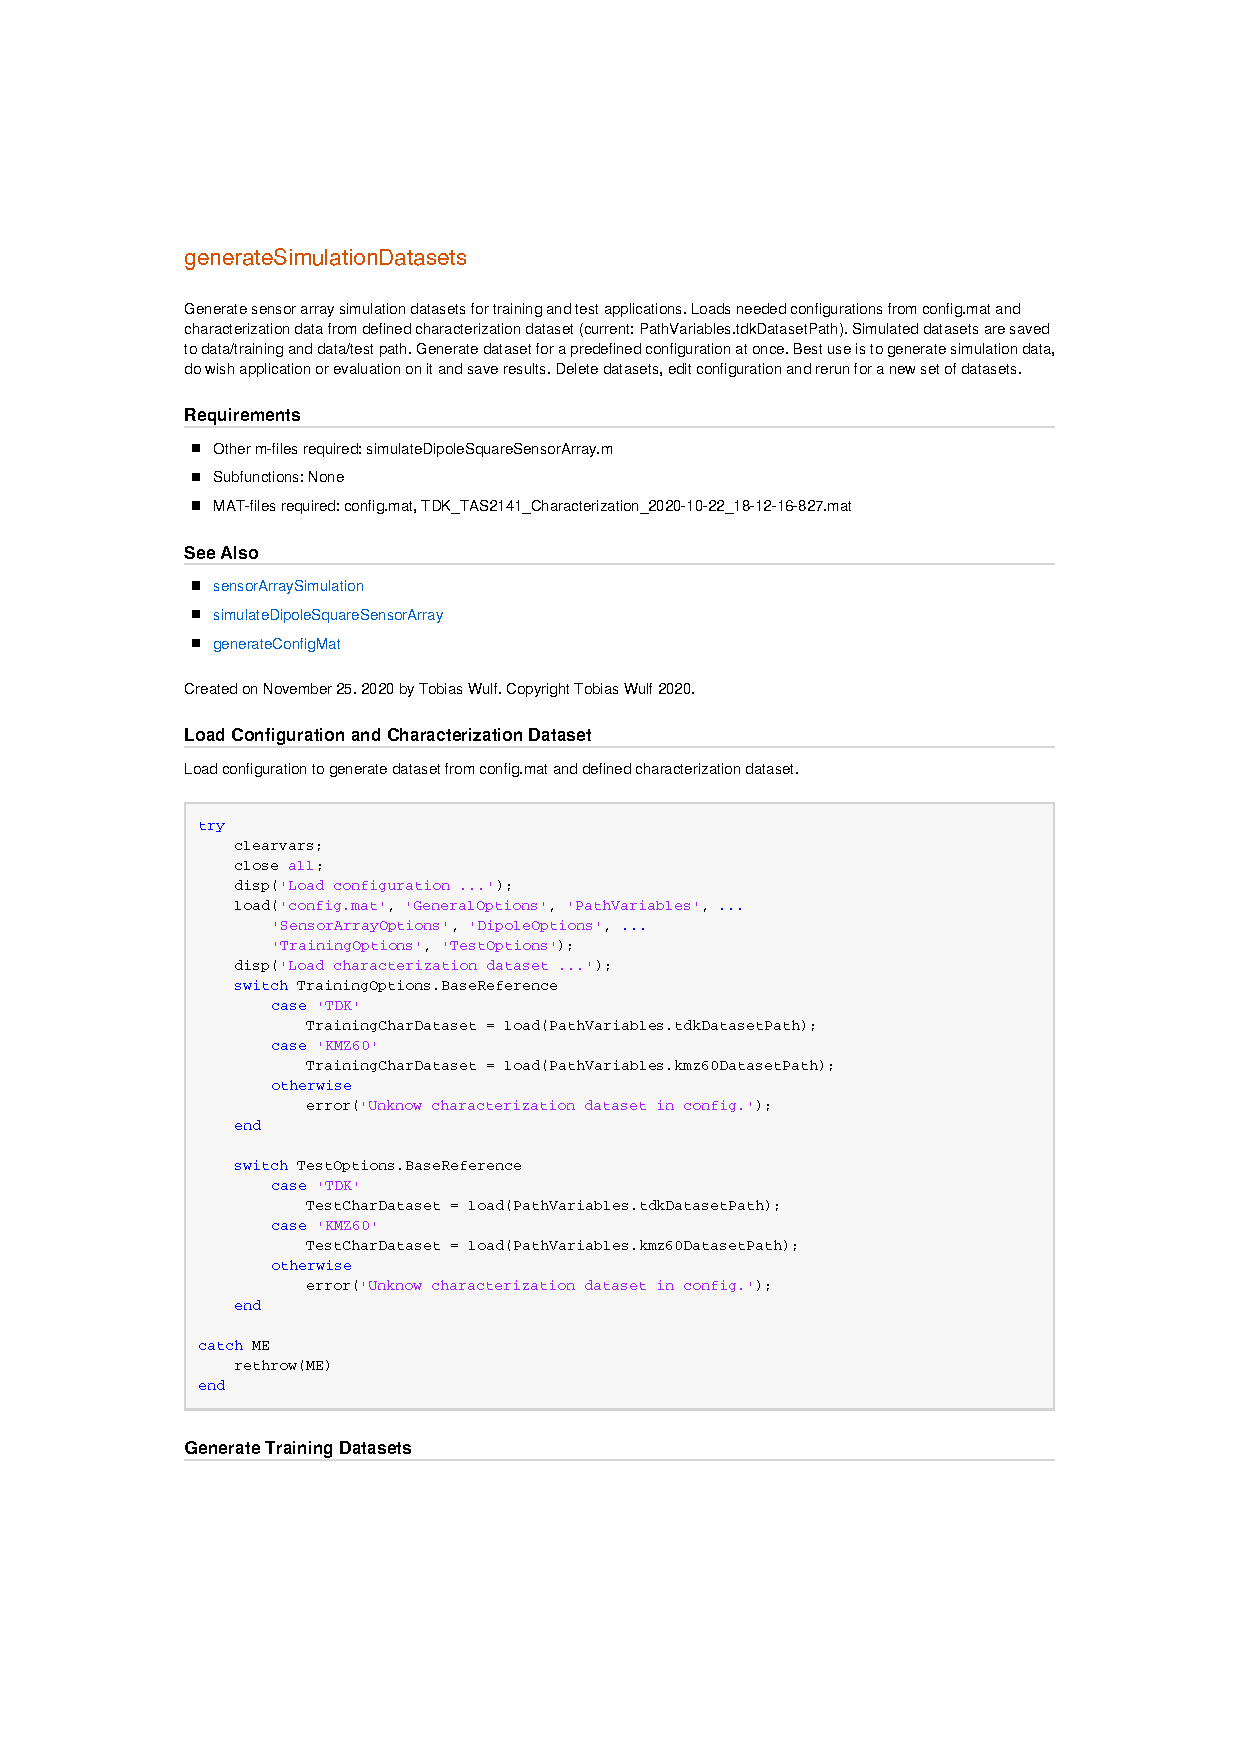
\includepdf[page=1,pagecommand={\phantomsection\addcontentsline{toc}{subsection}{\protect\numberline{\thesubsection}generateSimulationDatasets}\label{generateSimulationDatasets}}]{generateSimulationDatasets.pdf}
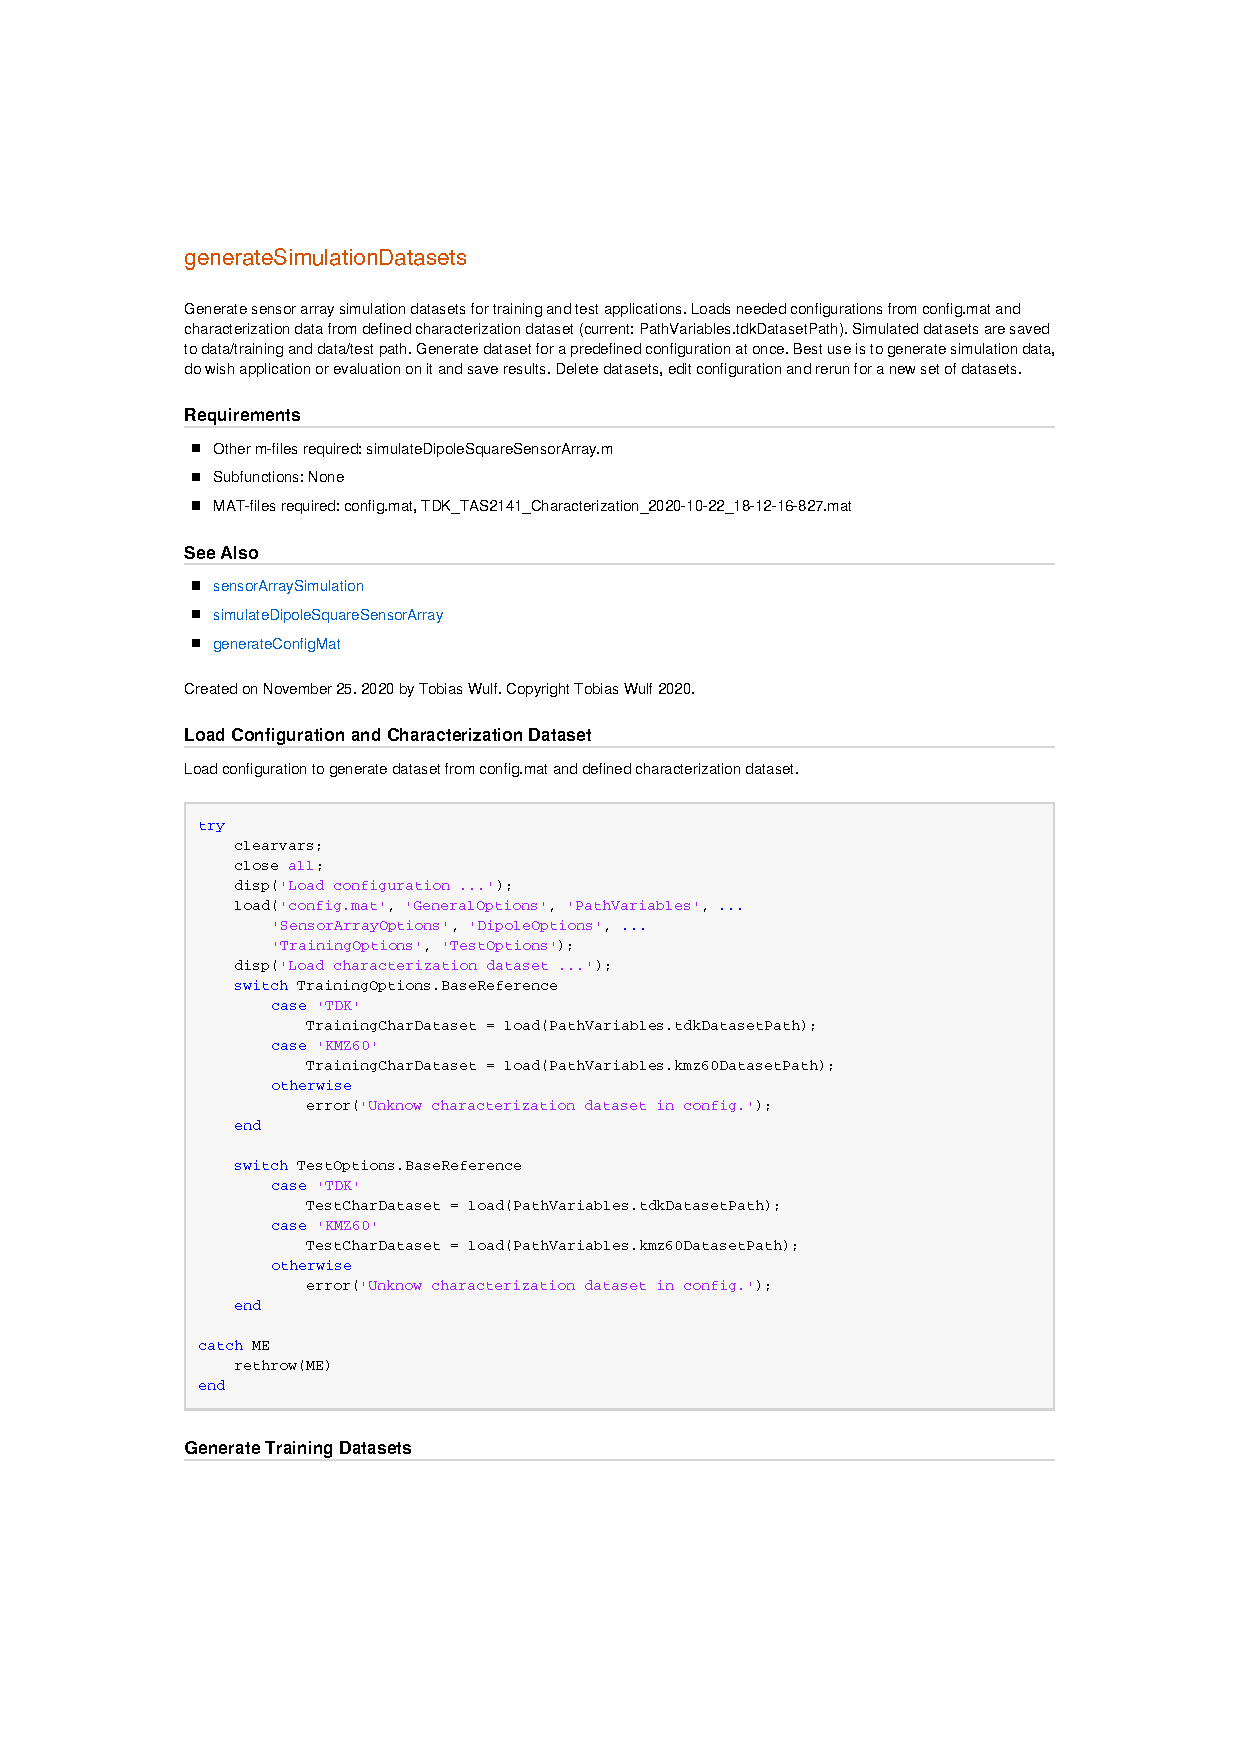
\includepdf[page=2-, pagecommand={\phantomsection}]{generateSimulationDatasets.pdf}
\addtocounter{subsection}{1}
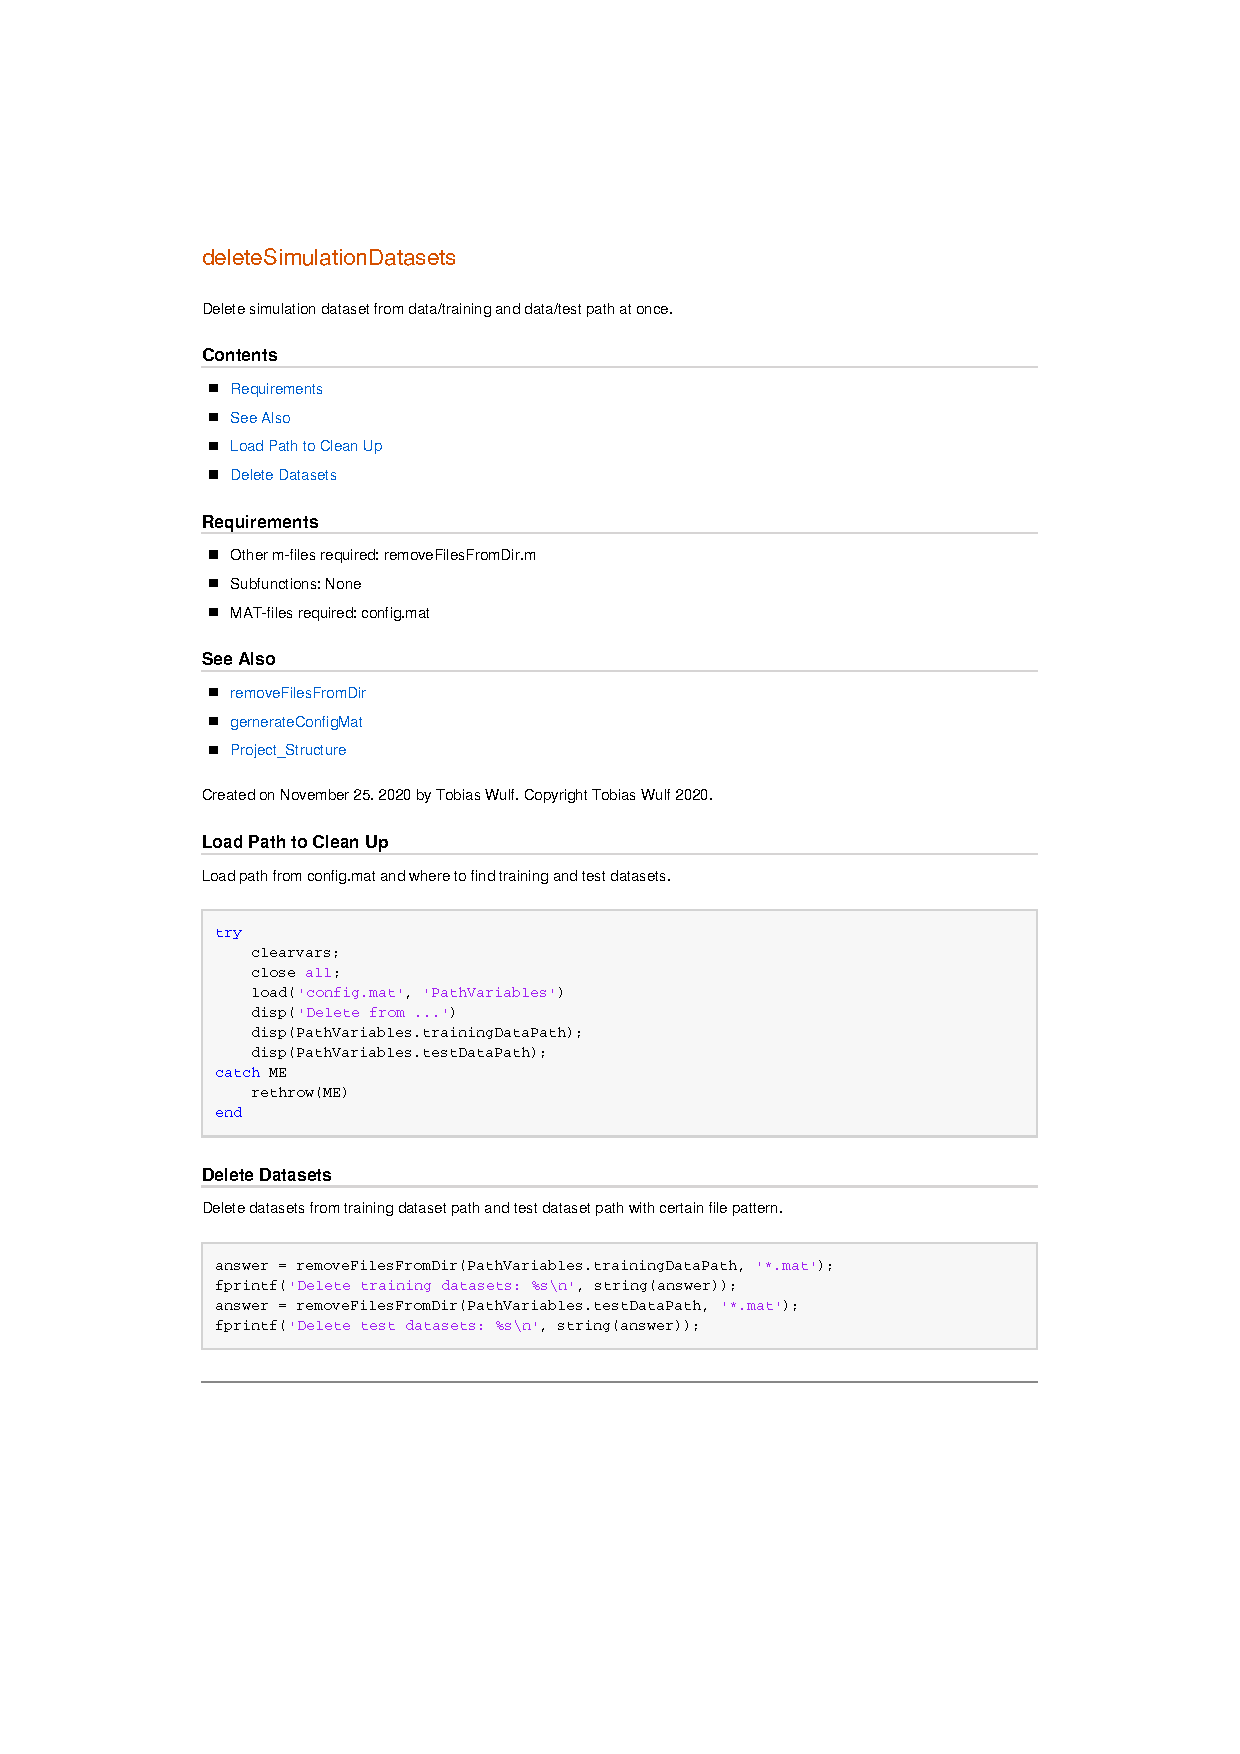
\includepdf[page=1,pagecommand={\phantomsection\addcontentsline{toc}{subsection}{\protect\numberline{\thesubsection}deleteSimulationDatasets}\label{deleteSimulationDatasets}}]{deleteSimulationDatasets.pdf}
\addtocounter{subsection}{1}
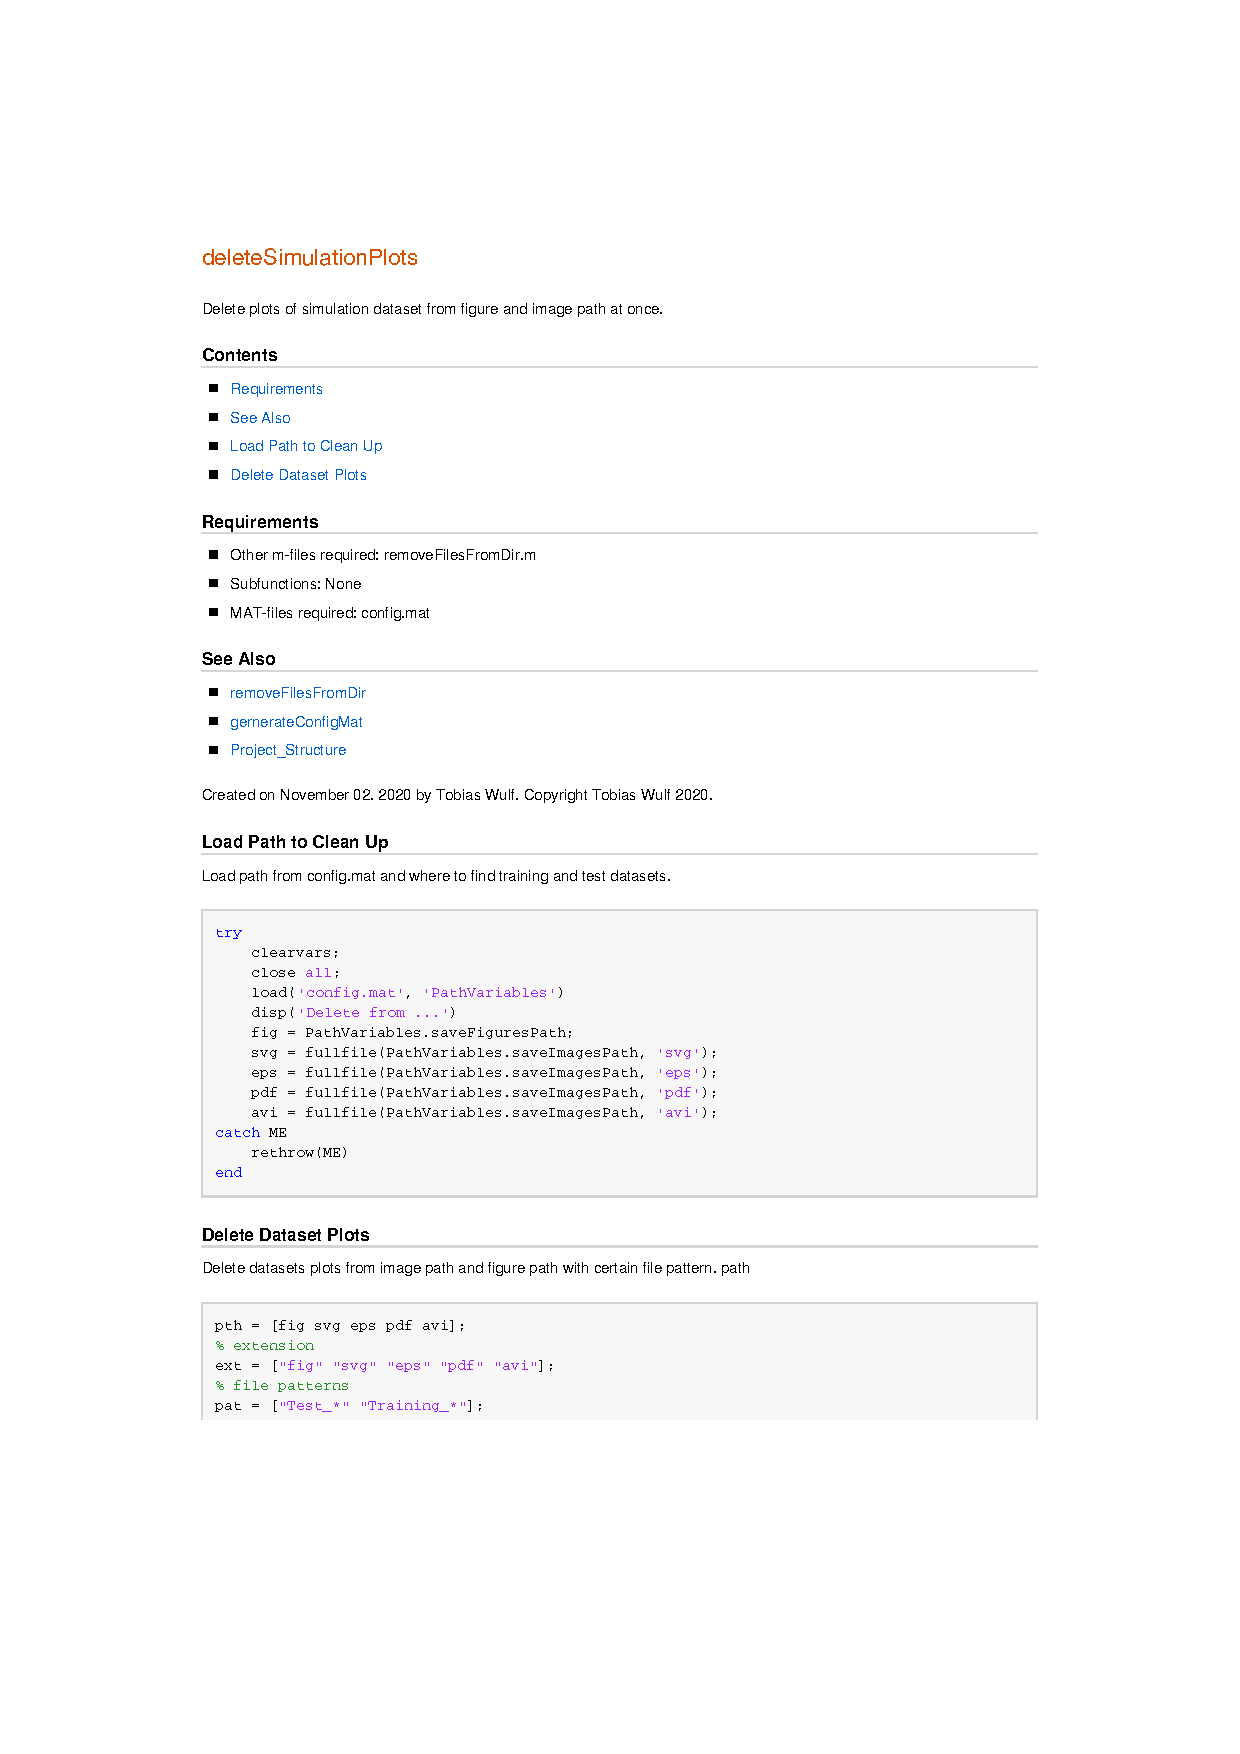
\includepdf[page=1,pagecommand={\phantomsection\addcontentsline{toc}{subsection}{\protect\numberline{\thesubsection}deleteSimulationPlots}\label{deleteSimulationPlots}}]{deleteSimulationPlots.pdf}
\addtocounter{subsection}{1}
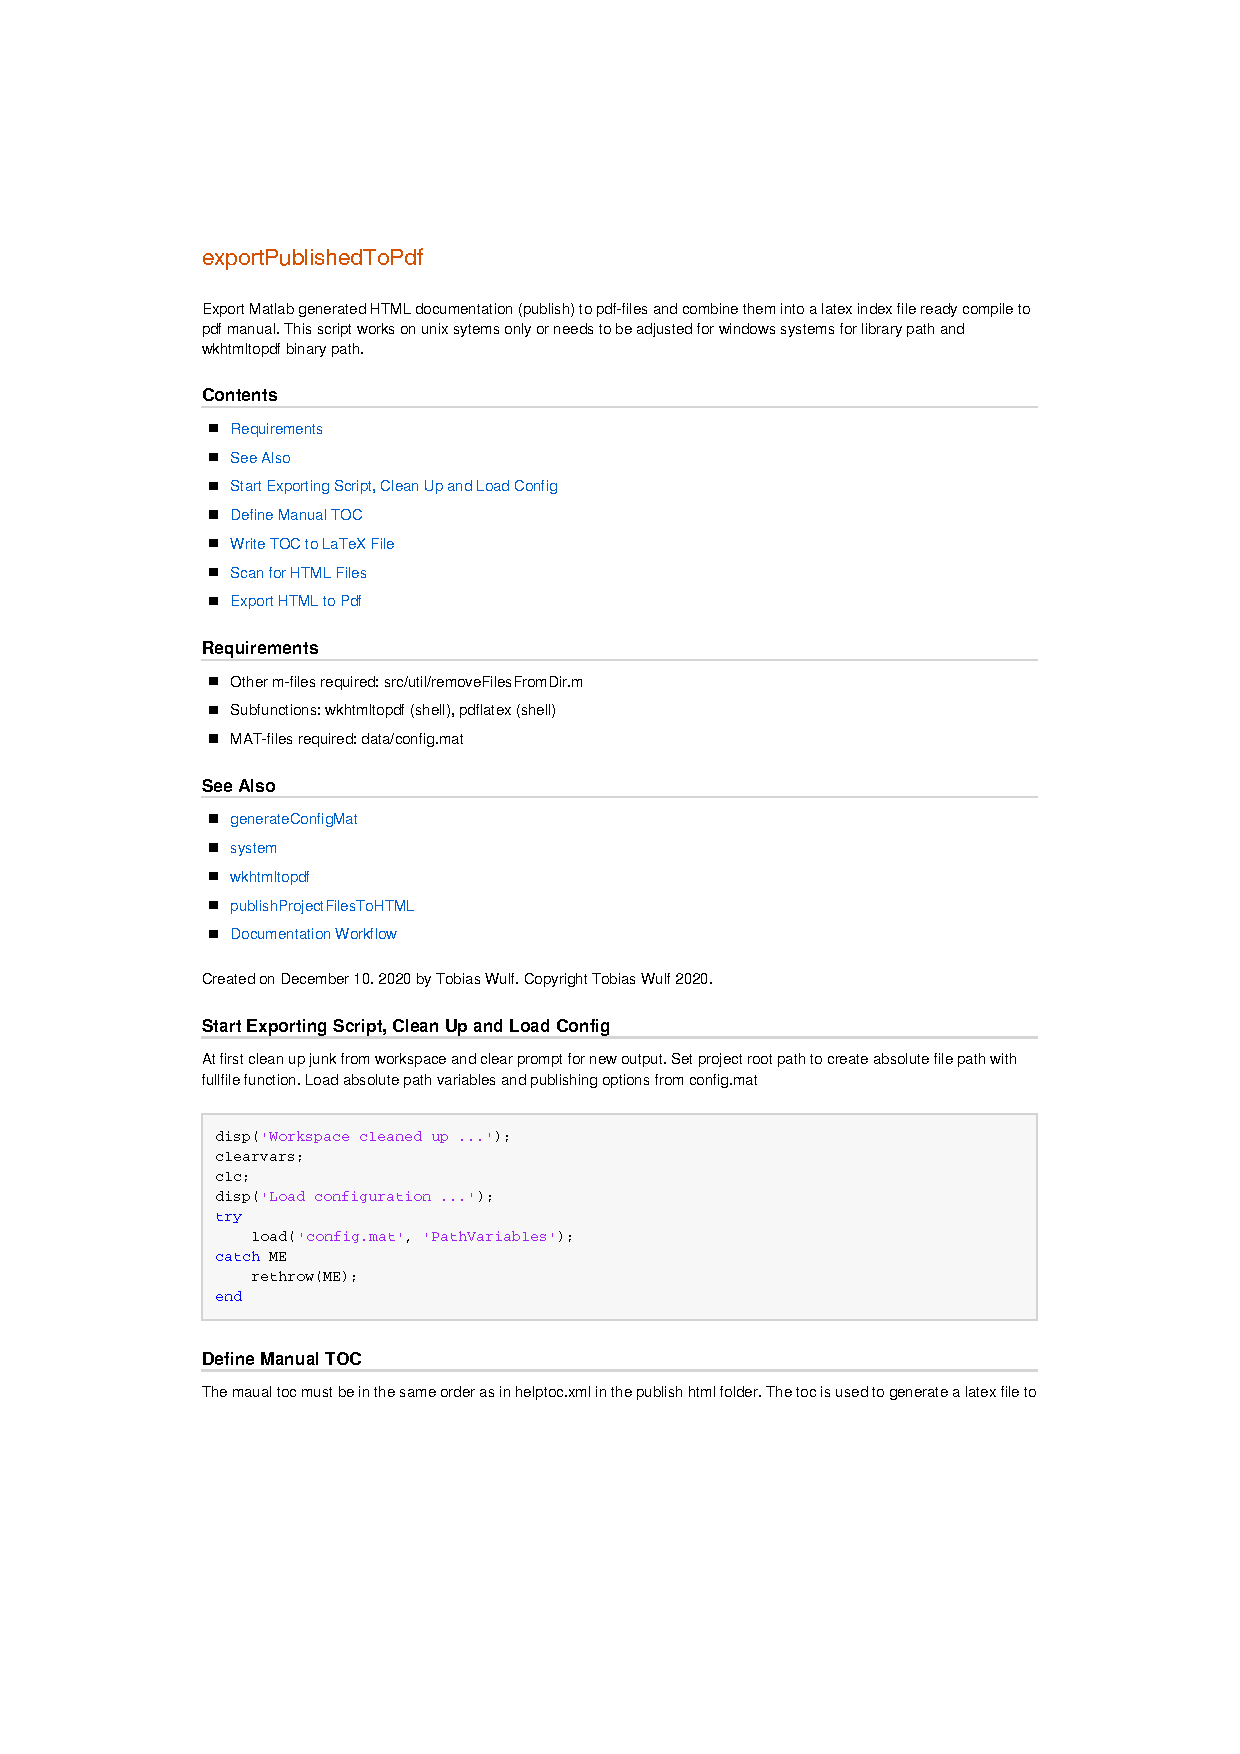
\includepdf[page=1,pagecommand={\phantomsection\addcontentsline{toc}{subsection}{\protect\numberline{\thesubsection}exportPublishedToPdf}\label{exportPublishedToPdf}}]{exportPublishedToPdf.pdf}
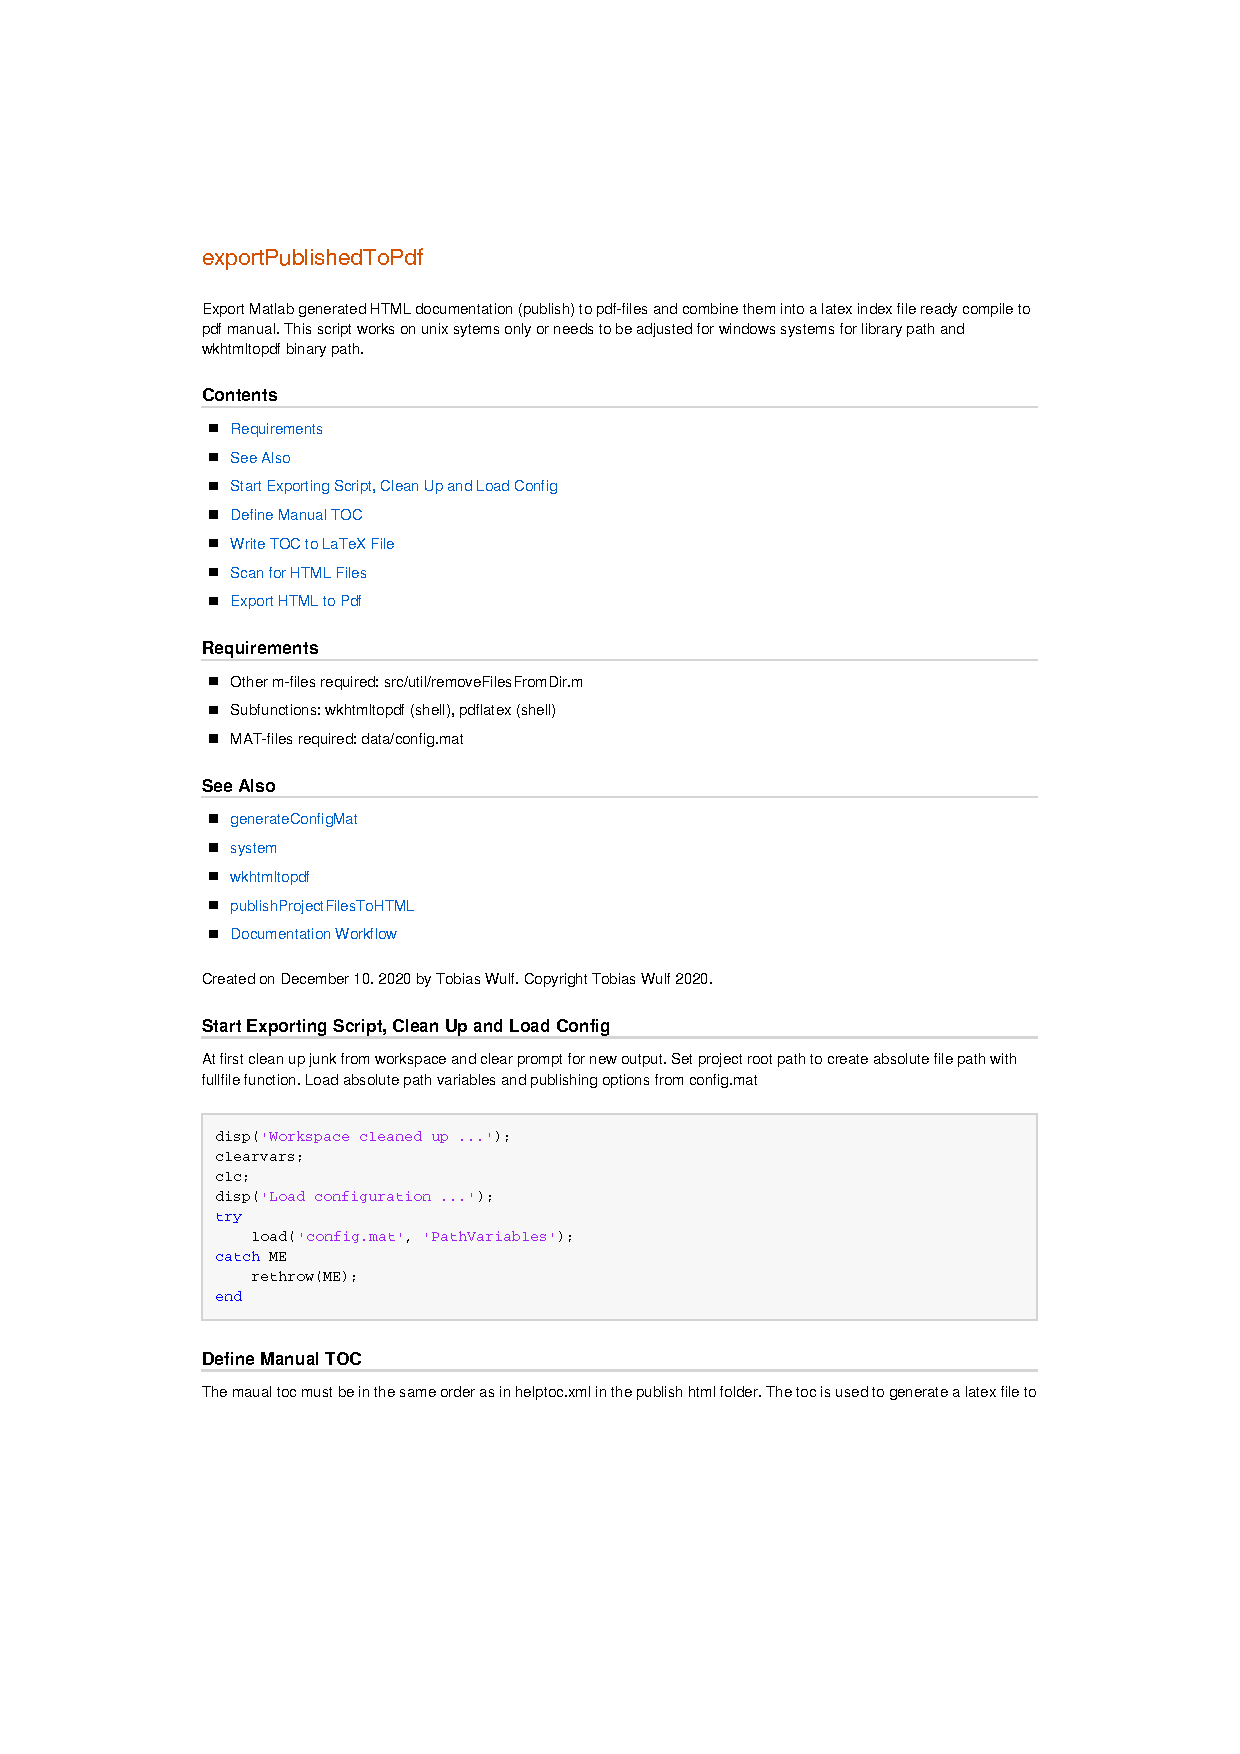
\includepdf[page=2-, pagecommand={\phantomsection}]{exportPublishedToPdf.pdf}
\addtocounter{subsection}{1}
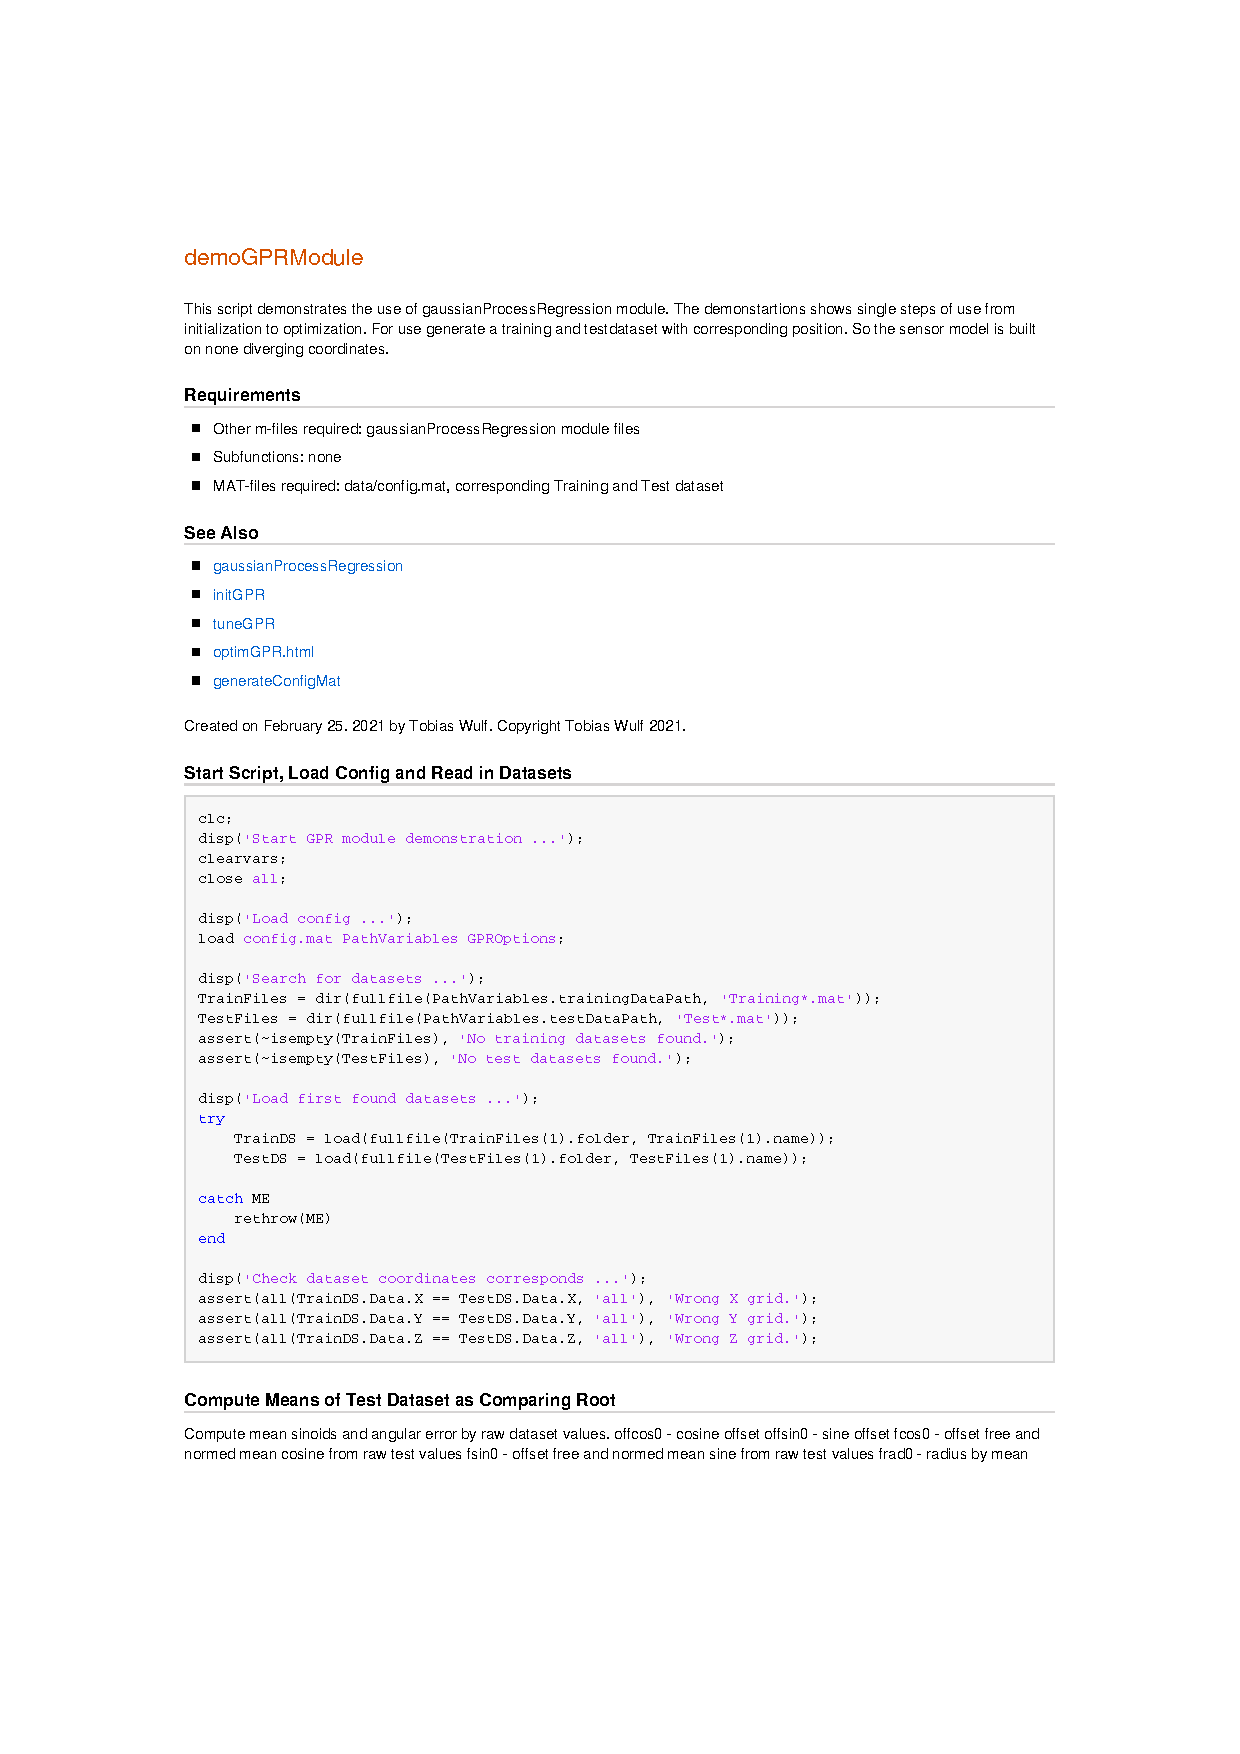
\includepdf[page=1,pagecommand={\phantomsection\addcontentsline{toc}{subsection}{\protect\numberline{\thesubsection}demoGPRModule}\label{demoGPRModule}}]{demoGPRModule.pdf}
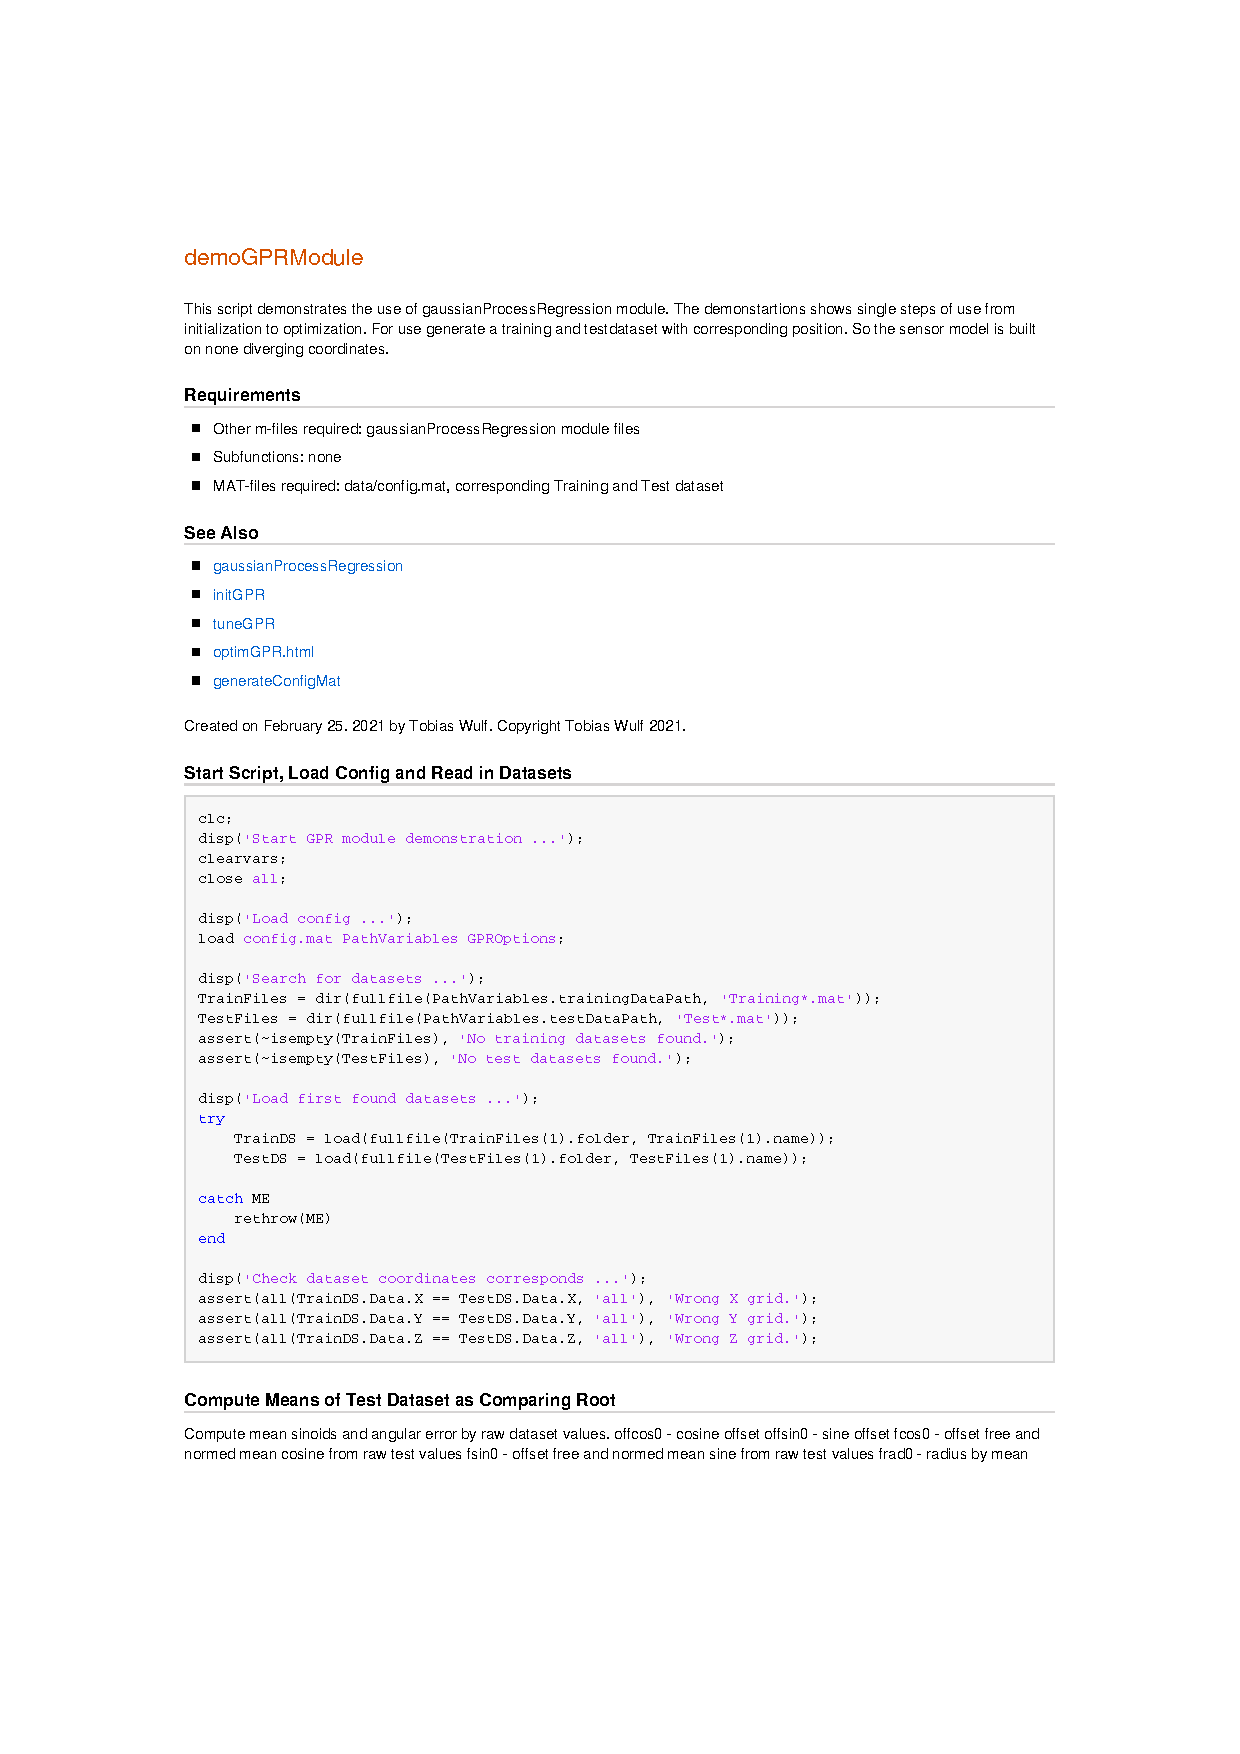
\includepdf[page=2-, pagecommand={\phantomsection}]{demoGPRModule.pdf}
\addtocounter{subsection}{1}
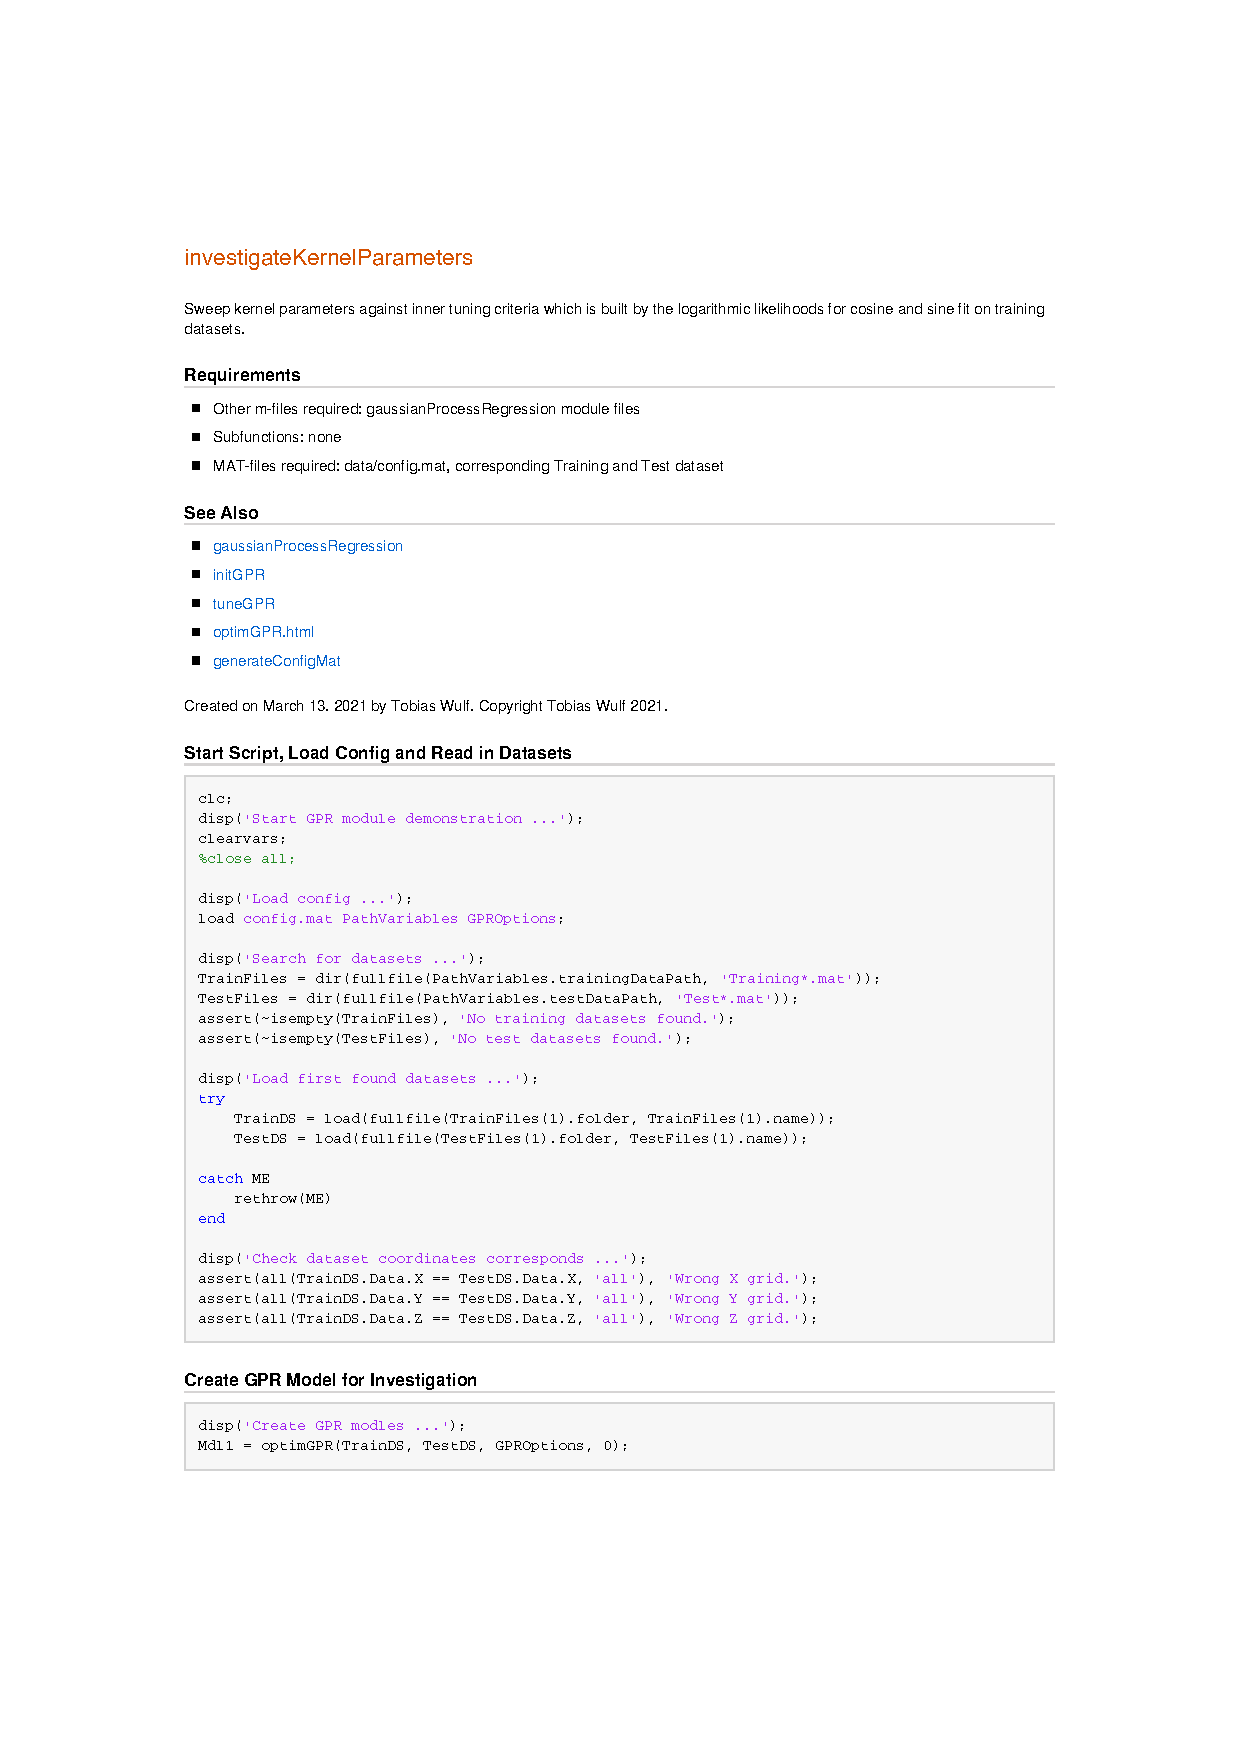
\includepdf[page=1,pagecommand={\phantomsection\addcontentsline{toc}{subsection}{\protect\numberline{\thesubsection}investigateKernelParameters}\label{investigateKernelParameters}}]{investigateKernelParameters.pdf}
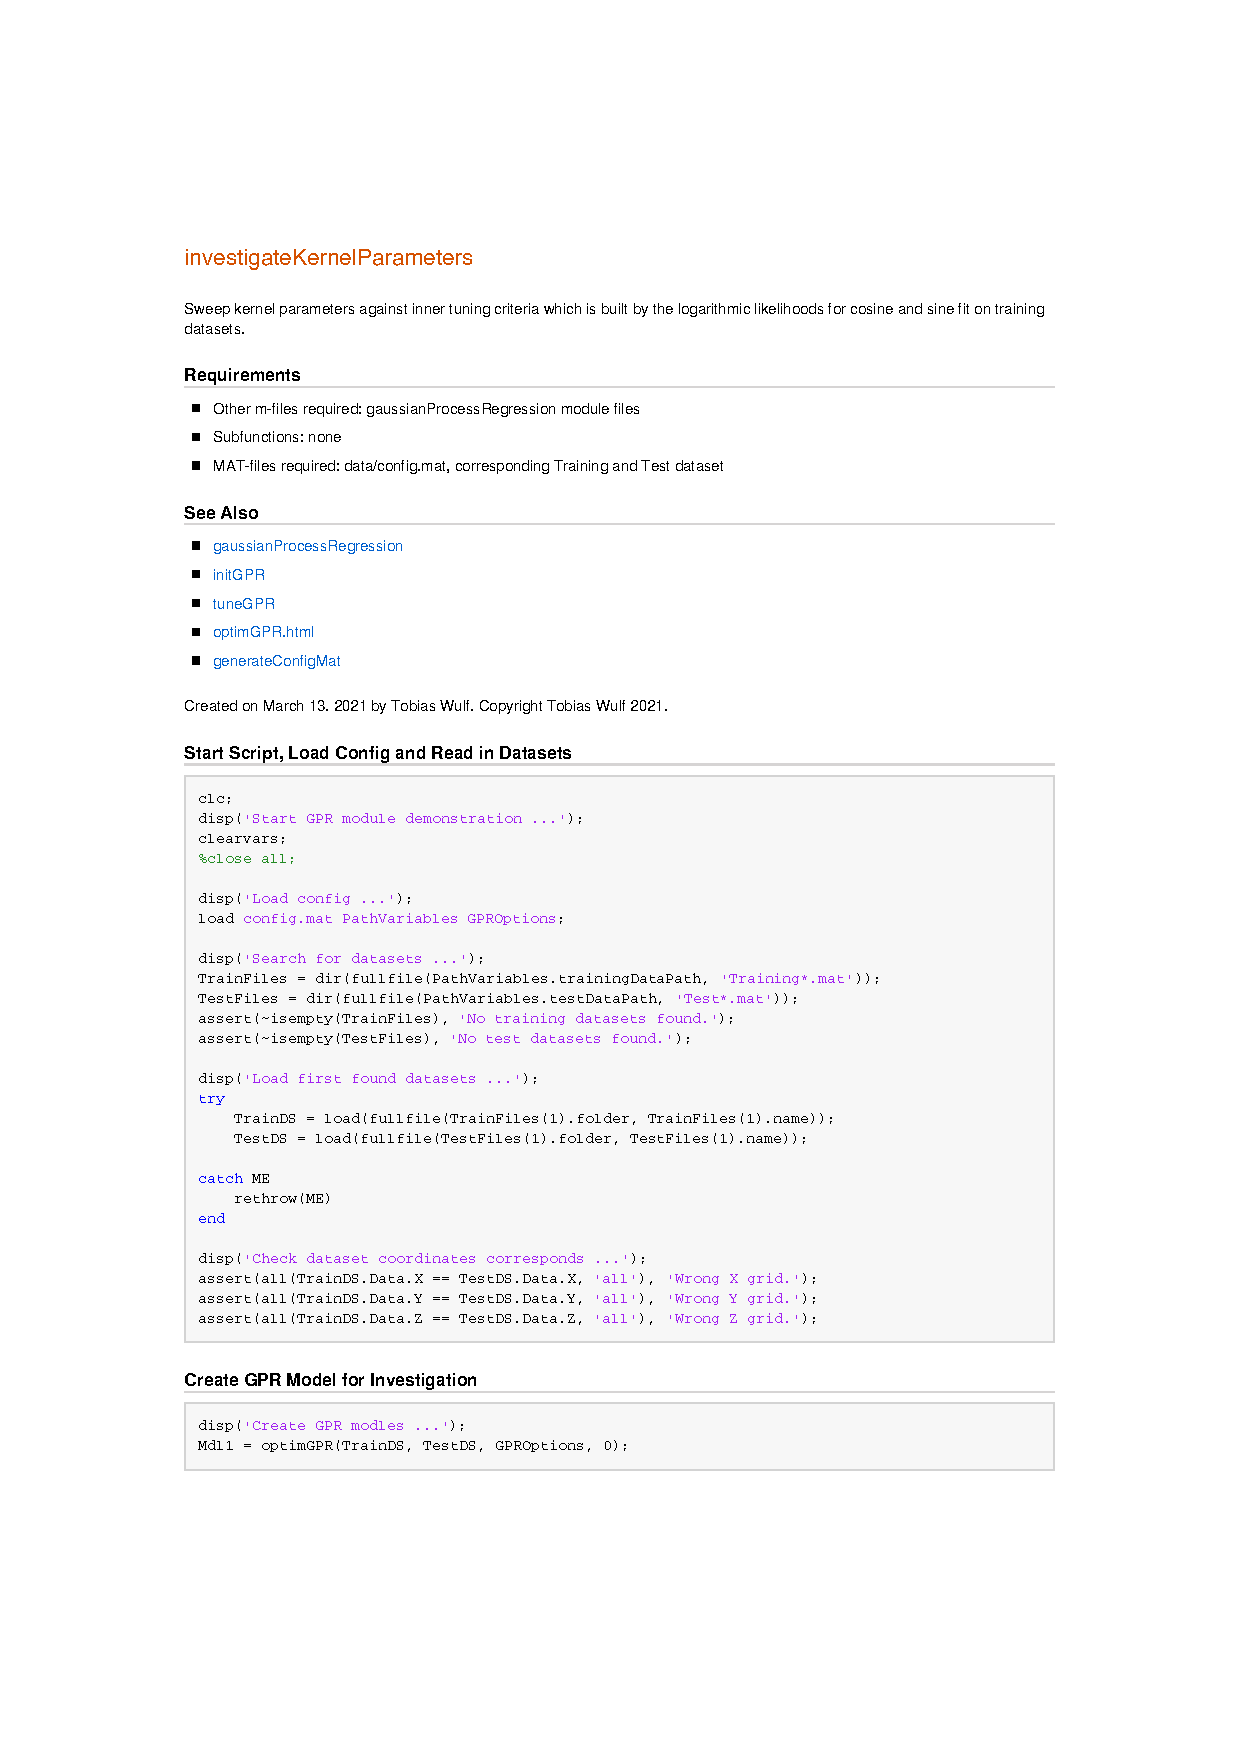
\includepdf[page=2-, pagecommand={\phantomsection}]{investigateKernelParameters.pdf}
\addtocounter{subsection}{1}
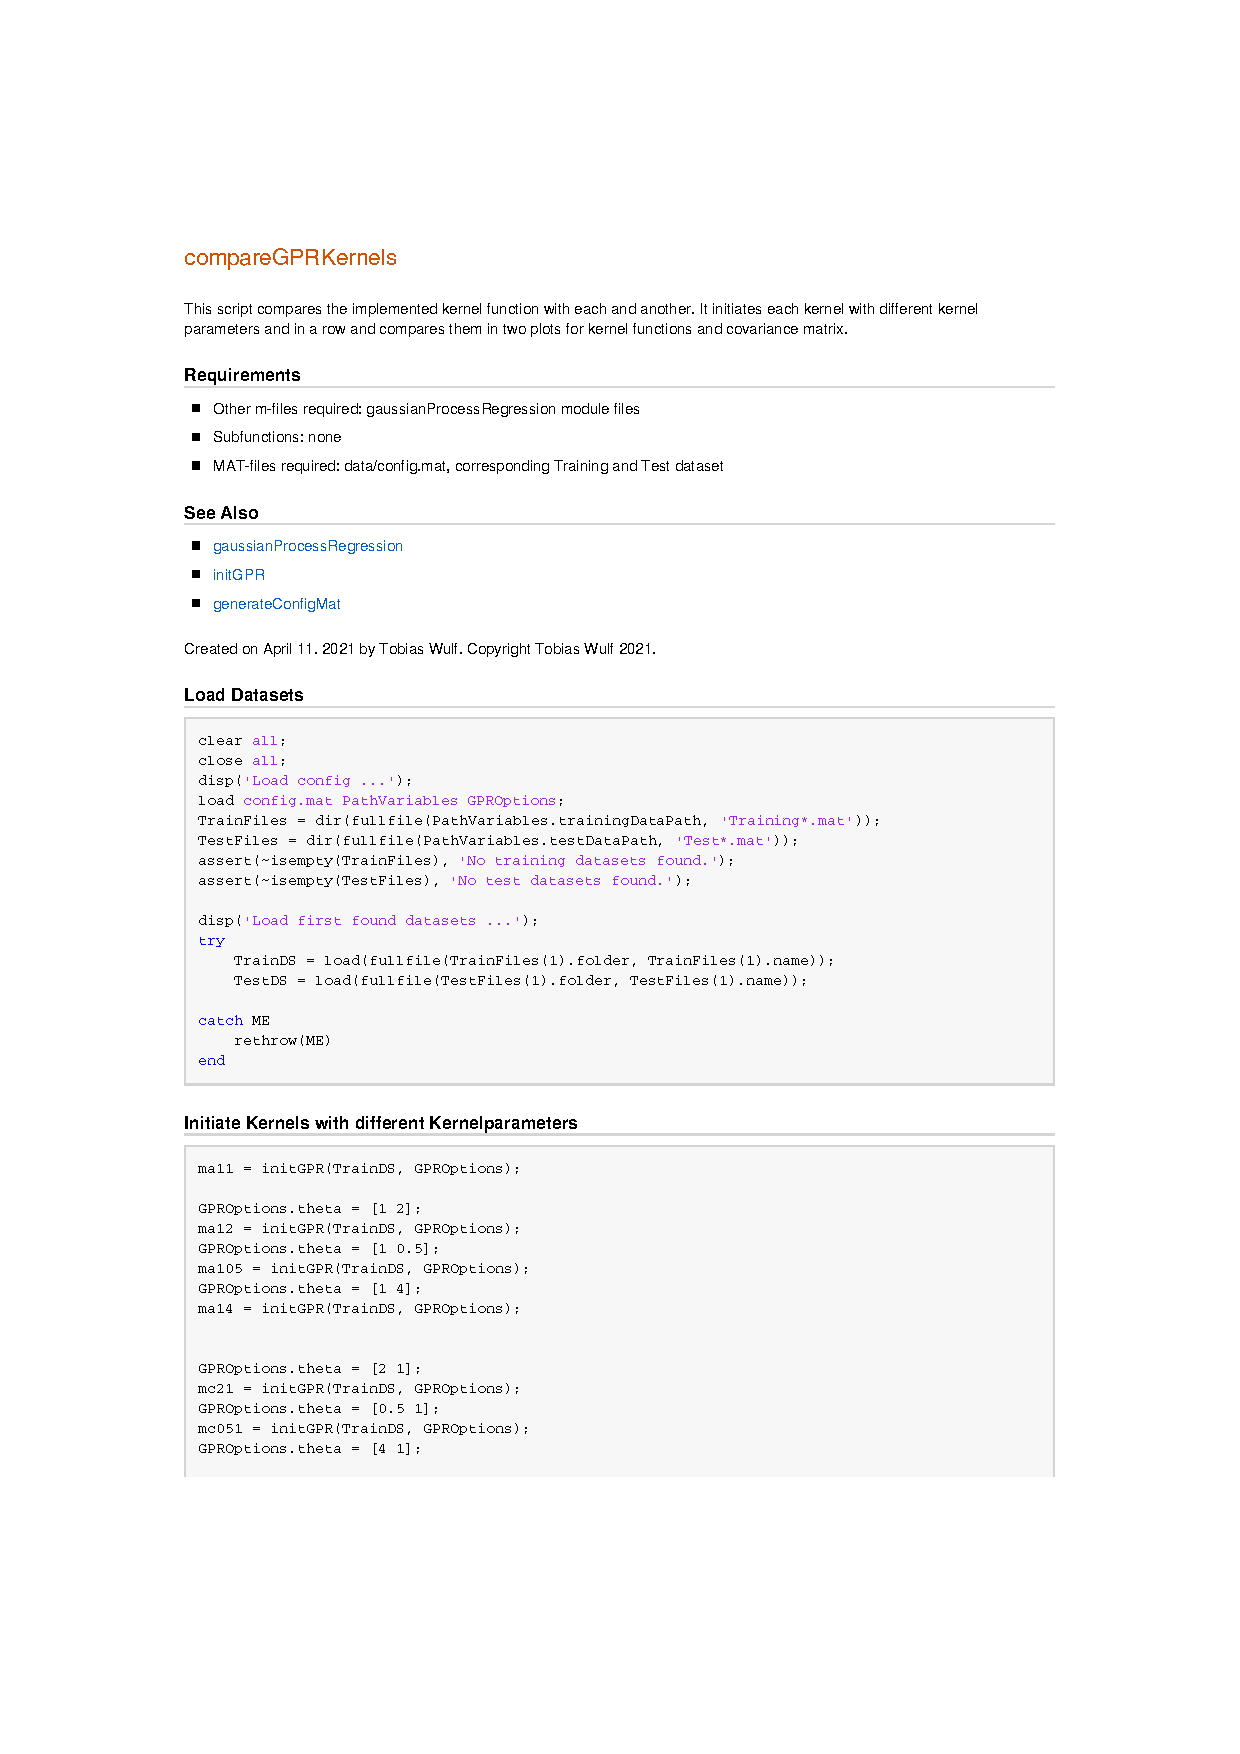
\includepdf[page=1,pagecommand={\phantomsection\addcontentsline{toc}{subsection}{\protect\numberline{\thesubsection}compareGPRKernels}\label{compareGPRKernels}}]{compareGPRKernels.pdf}
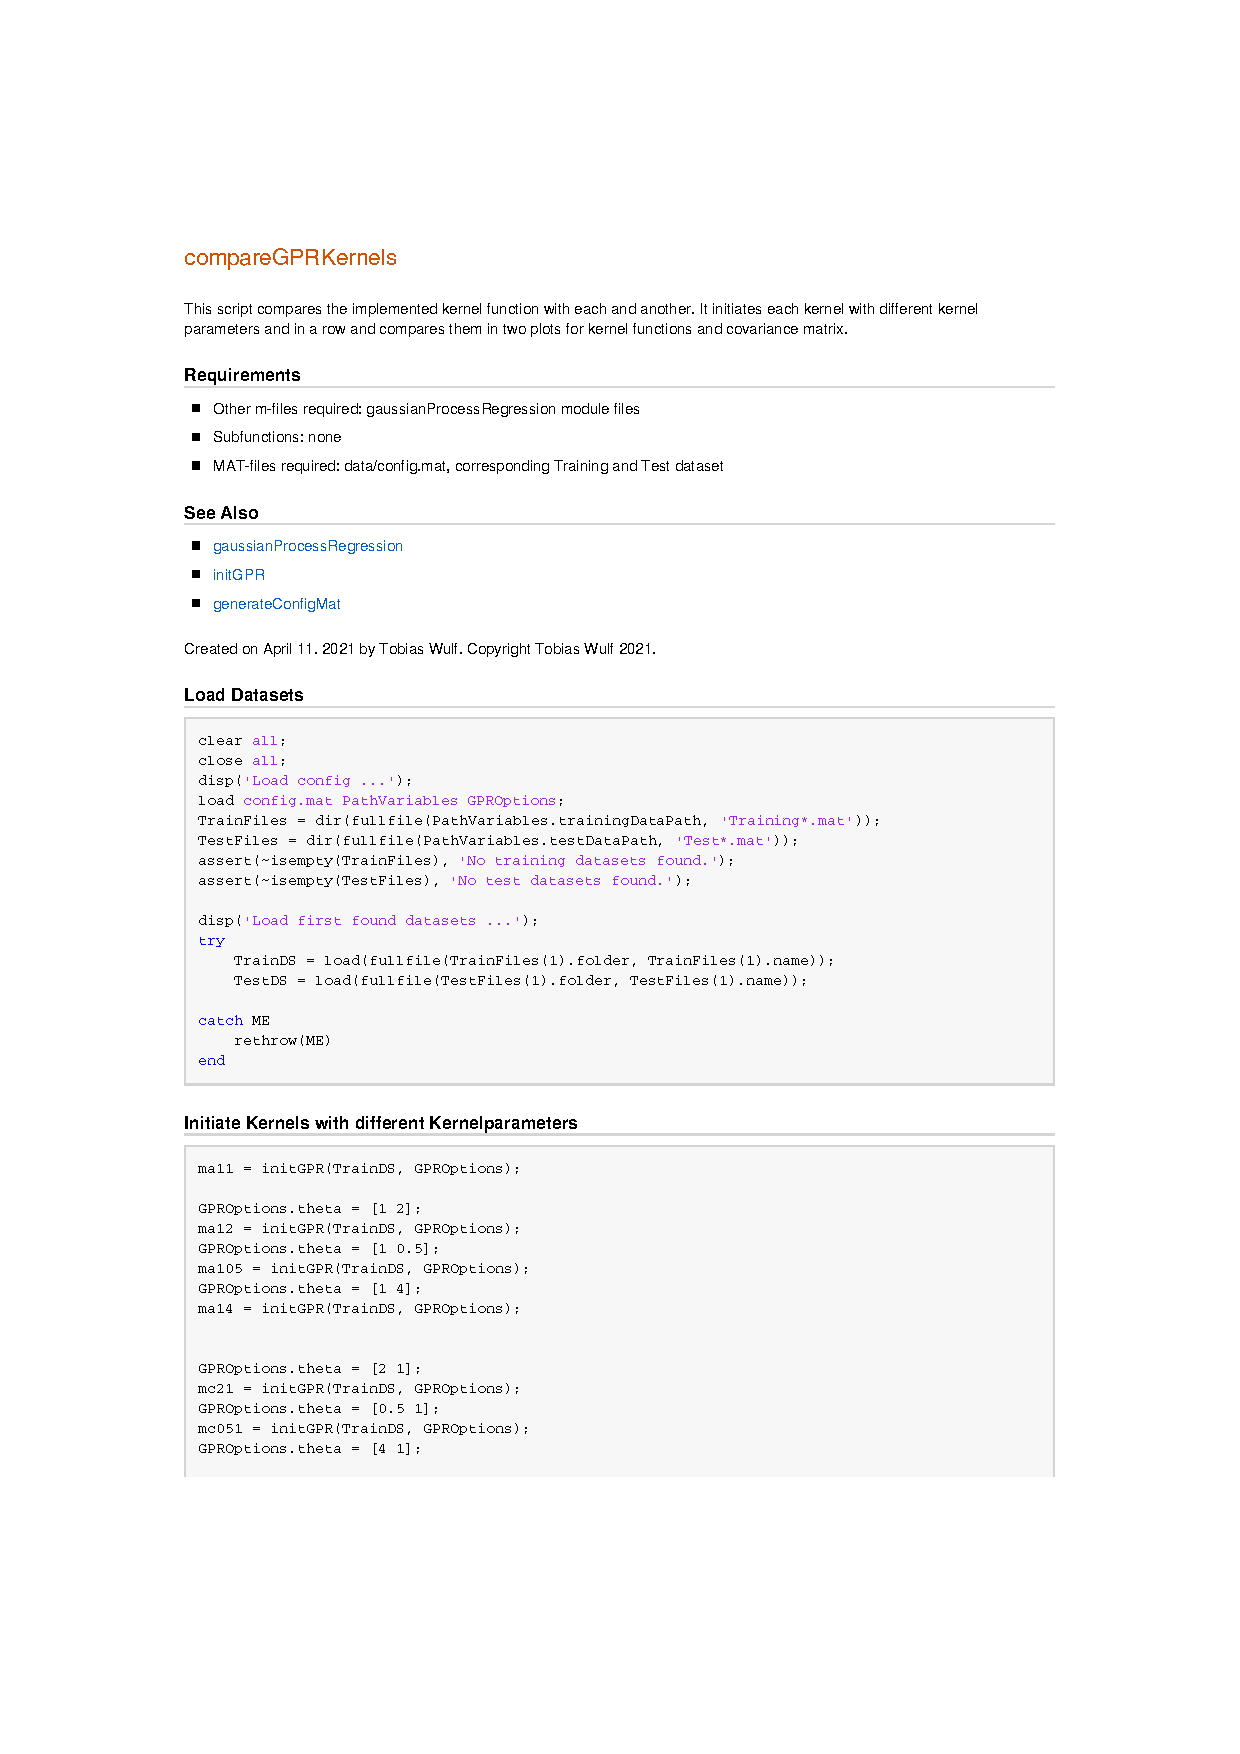
\includepdf[page=2-, pagecommand={\phantomsection}]{compareGPRKernels.pdf}
\addtocounter{section}{1}
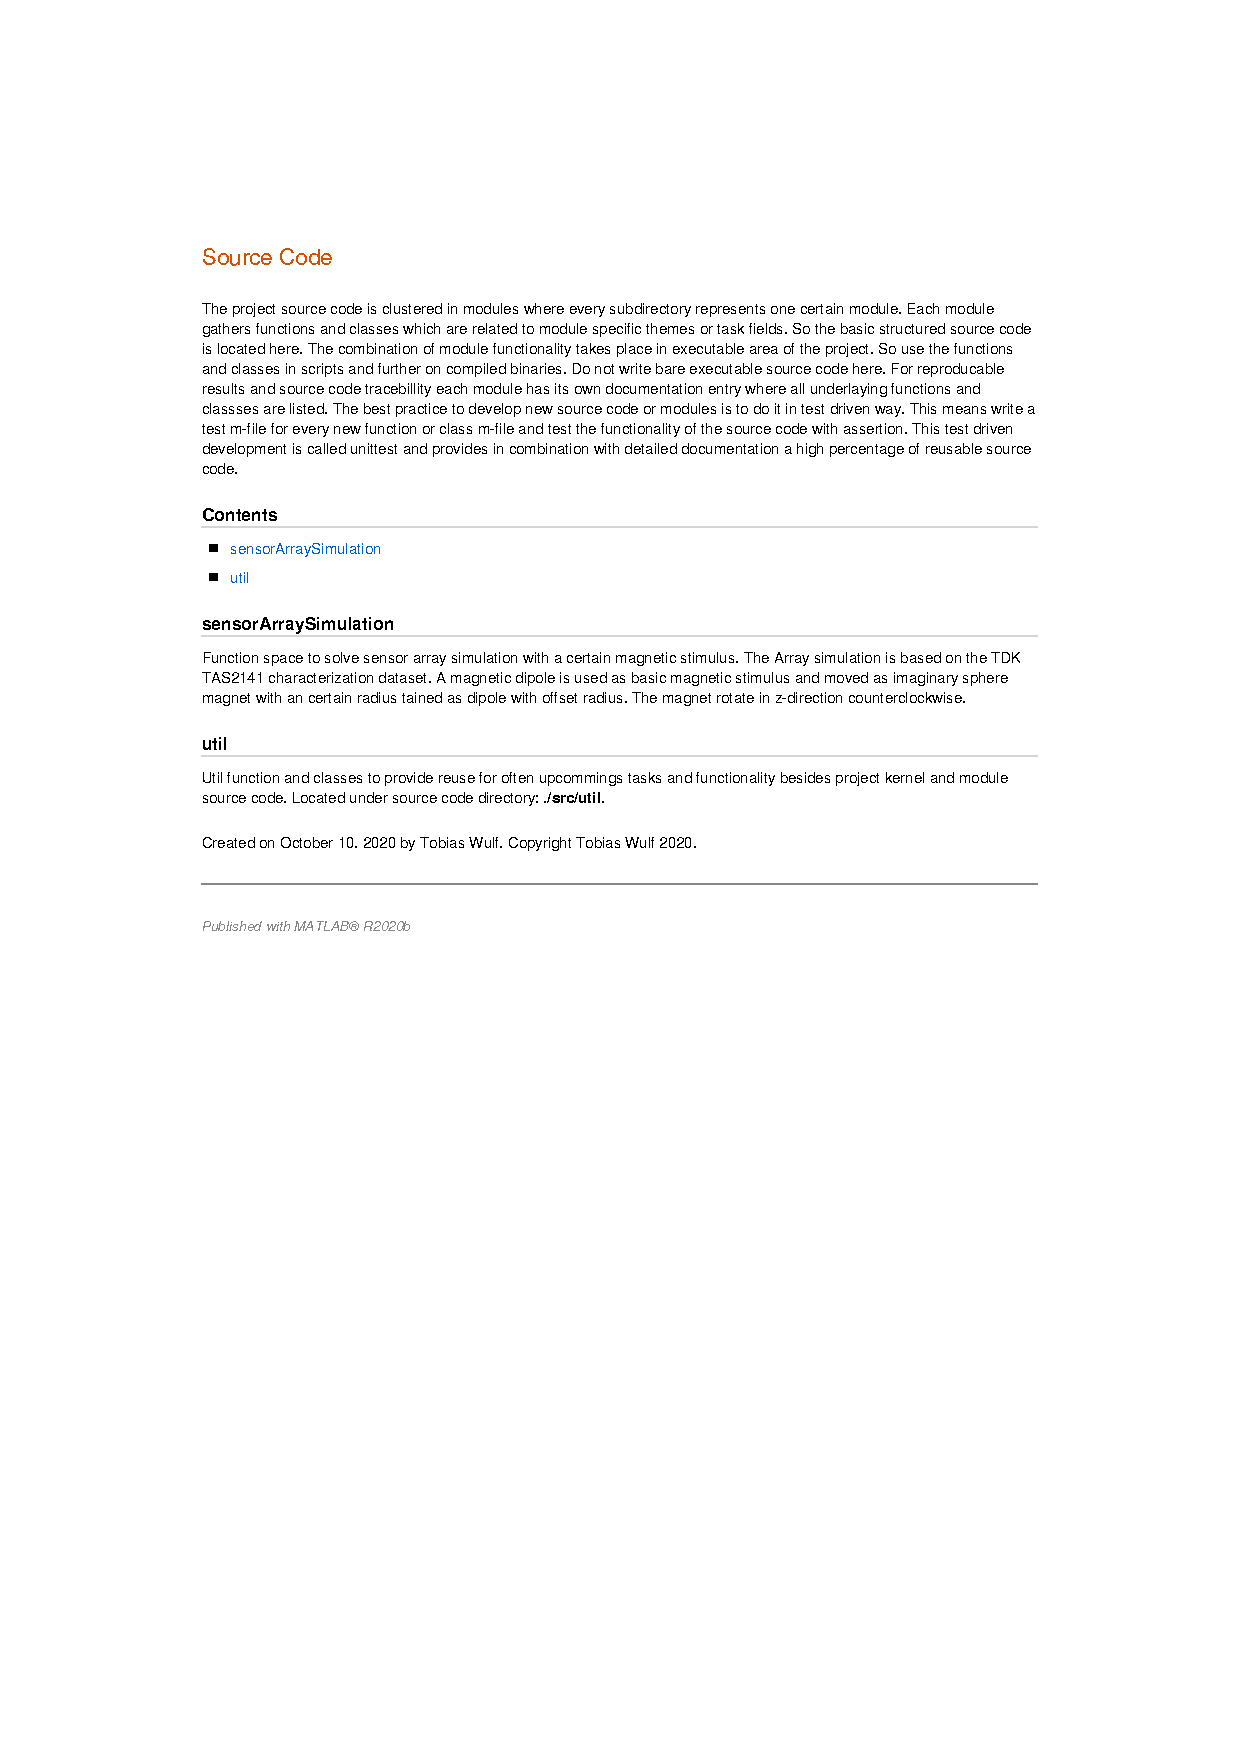
\includepdf[page=1,pagecommand={\phantomsection\addcontentsline{toc}{section}{\protect\numberline{\thesection}Source Code}\label{Source Code}}]{Source_Code.pdf}
\addtocounter{subsection}{1}
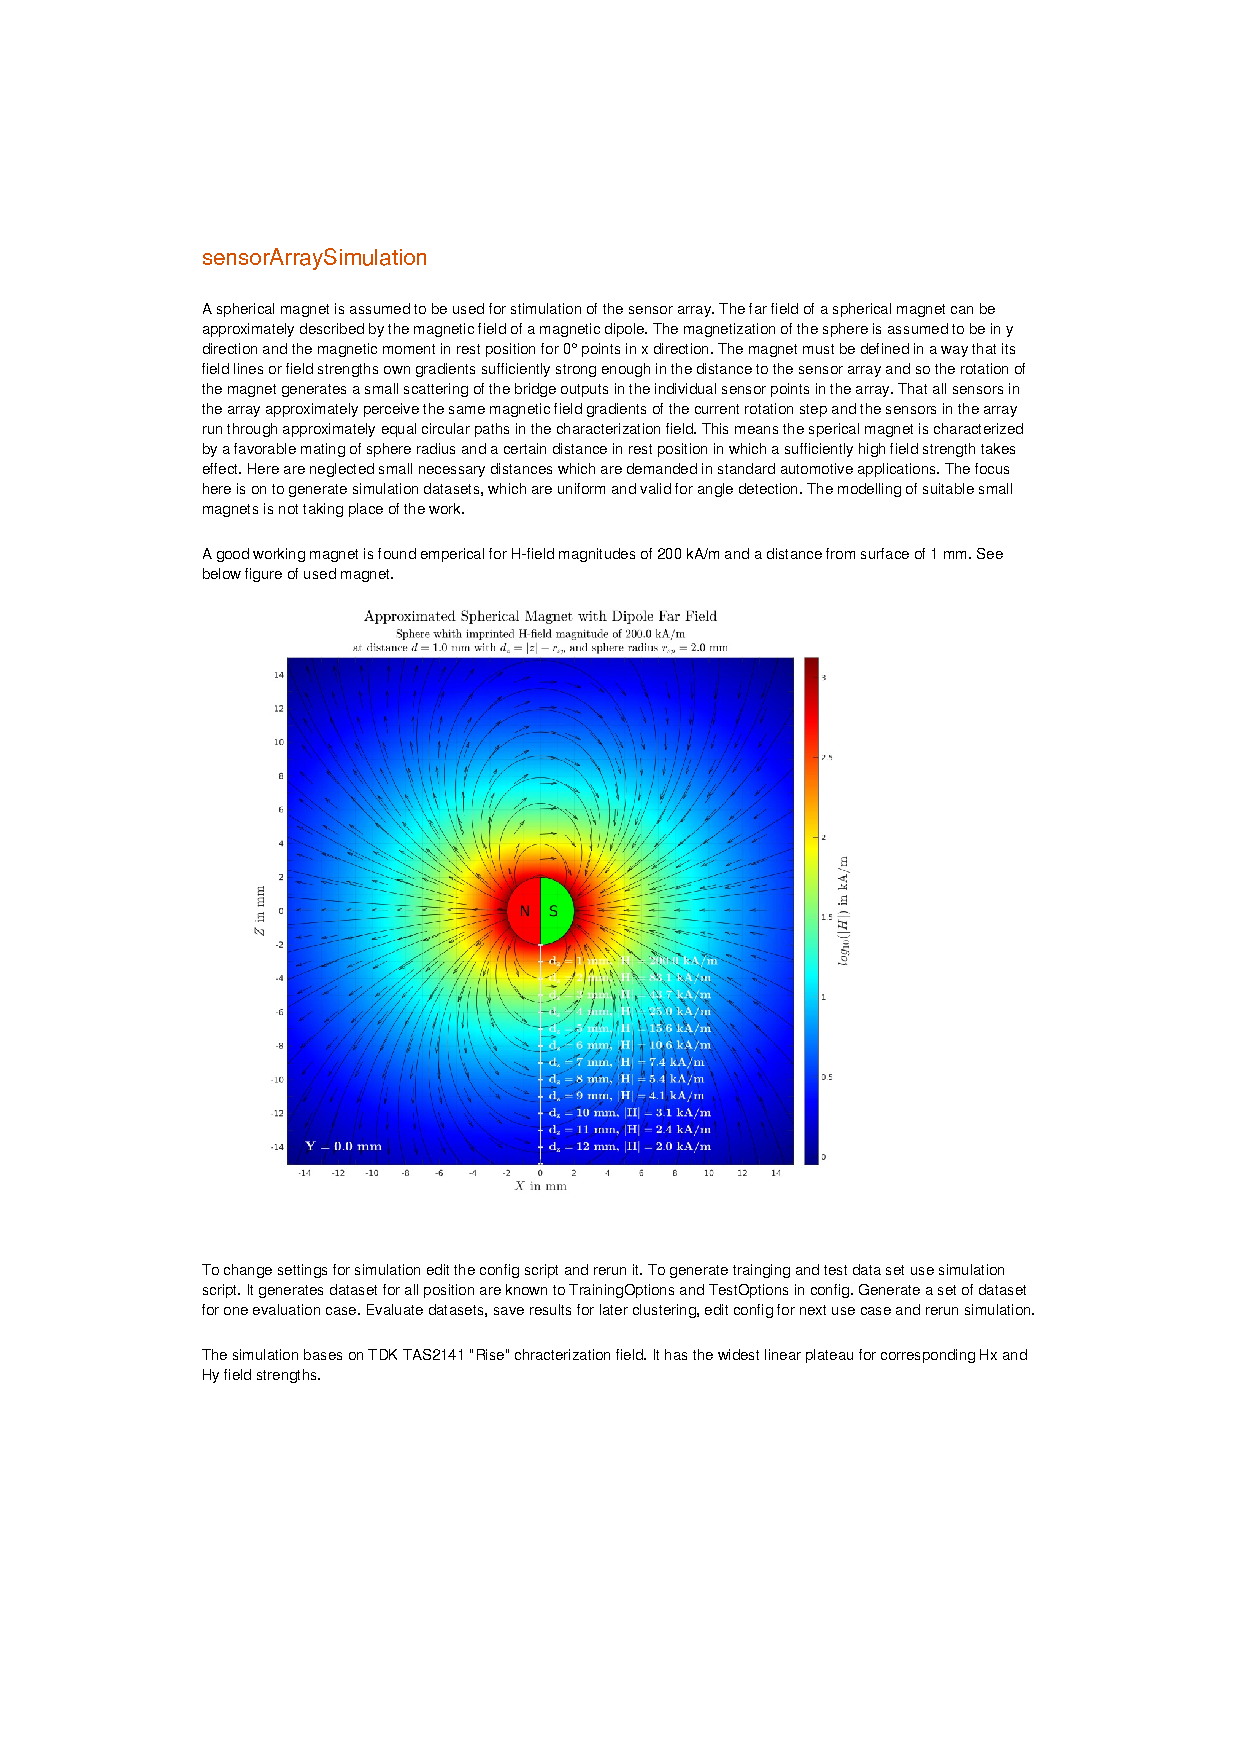
\includepdf[page=1,pagecommand={\phantomsection\addcontentsline{toc}{subsection}{\protect\numberline{\thesubsection}sensorArraySimulation}\label{sensorArraySimulation}}]{sensorArraySimulation.pdf}
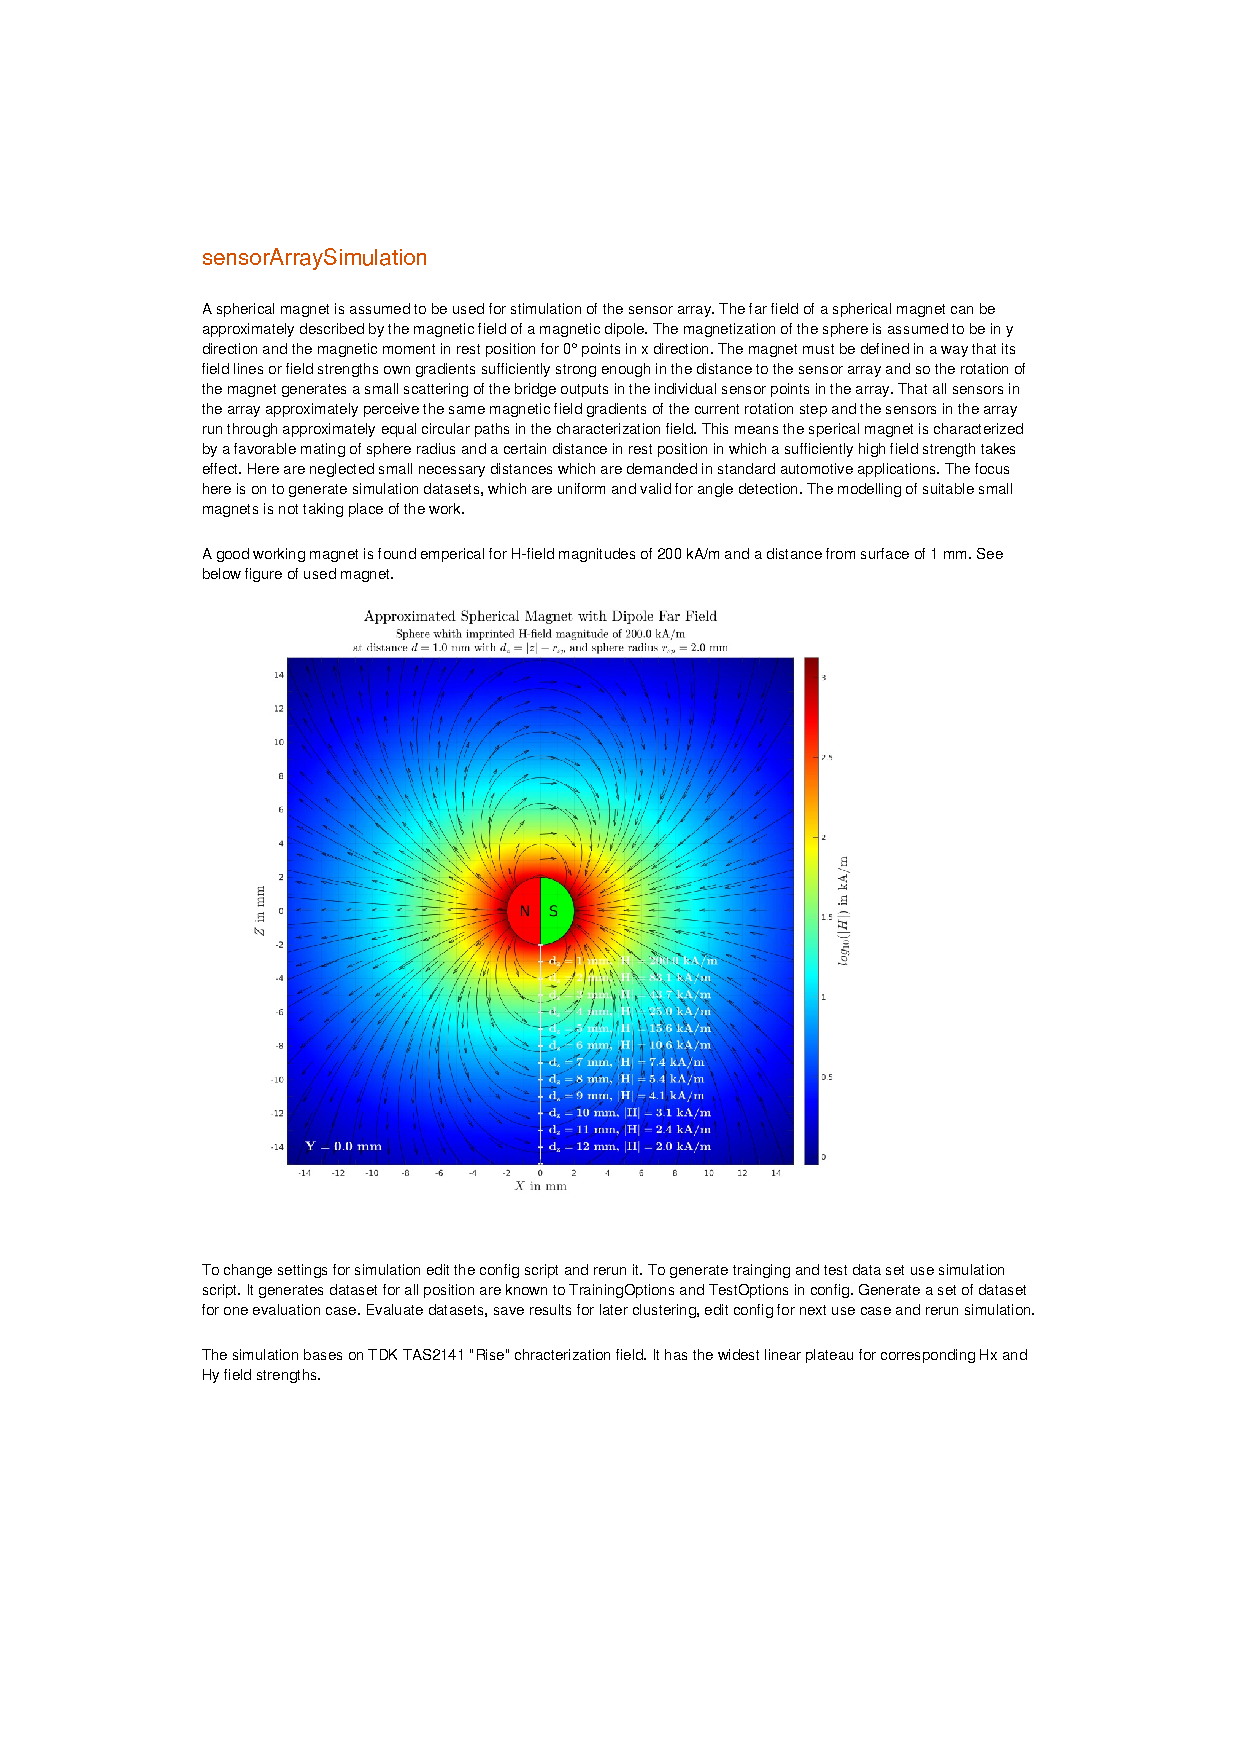
\includepdf[page=2-, pagecommand={\phantomsection}]{sensorArraySimulation.pdf}
\addtocounter{subsubsection}{1}
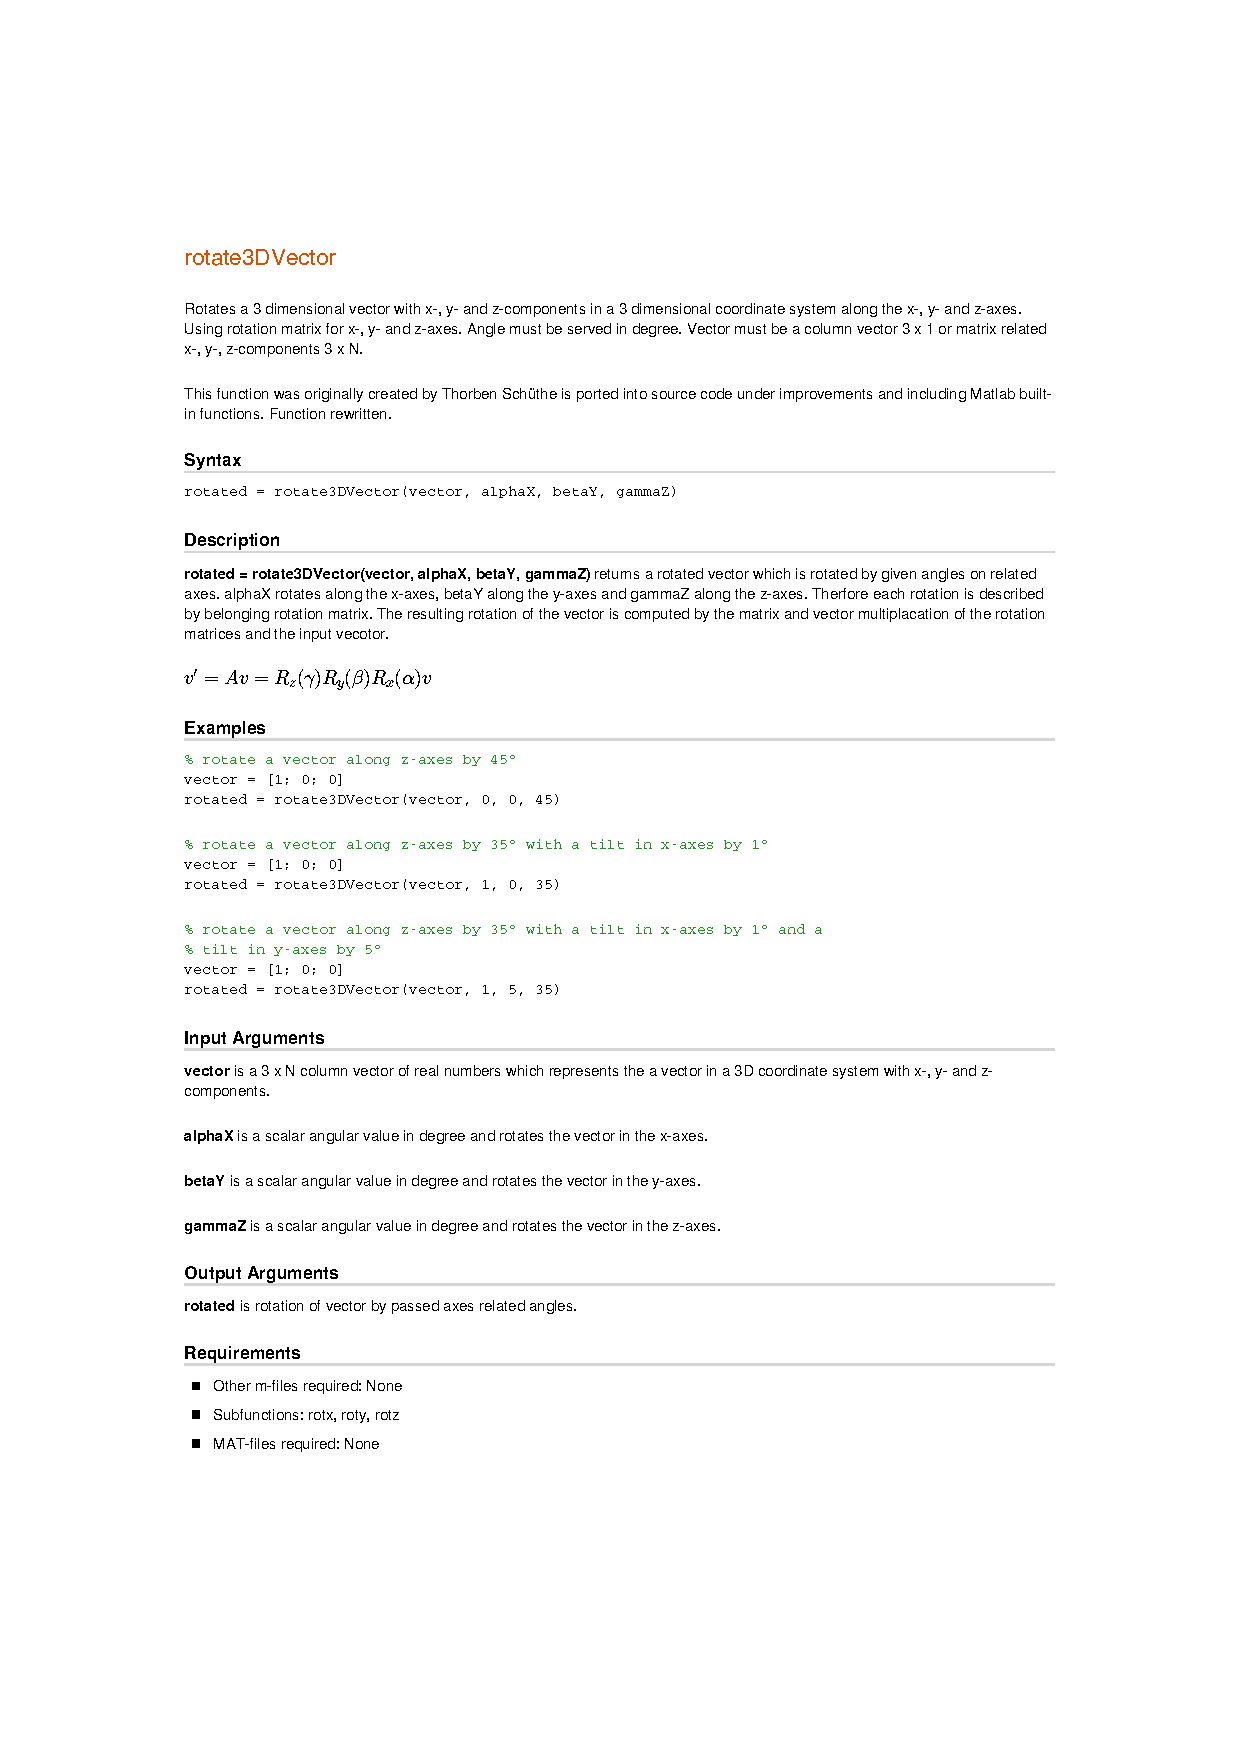
\includepdf[page=1,pagecommand={\phantomsection\addcontentsline{toc}{subsubsection}{\protect\numberline{\thesubsubsection}rotate3DVector}\label{rotate3DVector}}]{rotate3DVector.pdf}
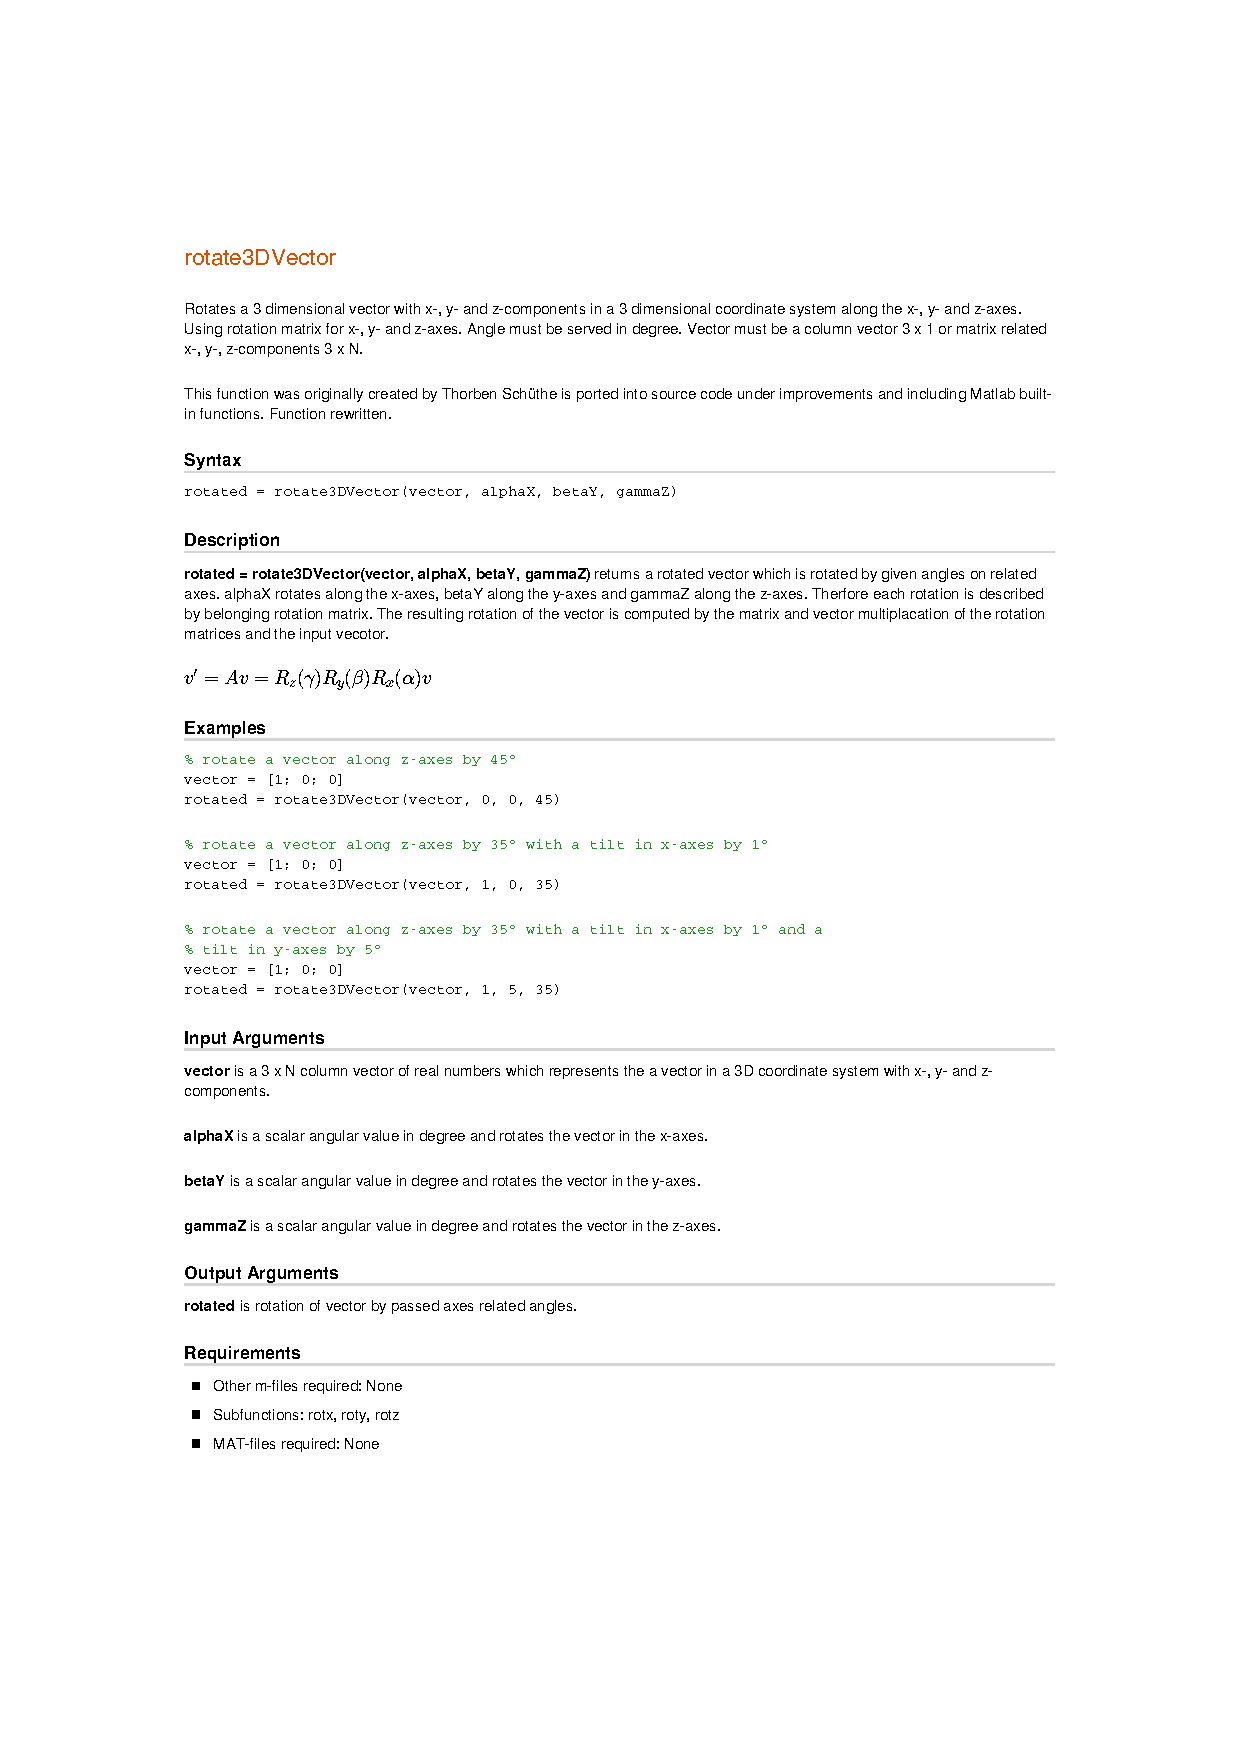
\includepdf[page=2-, pagecommand={\phantomsection}]{rotate3DVector.pdf}
\addtocounter{subsubsection}{1}
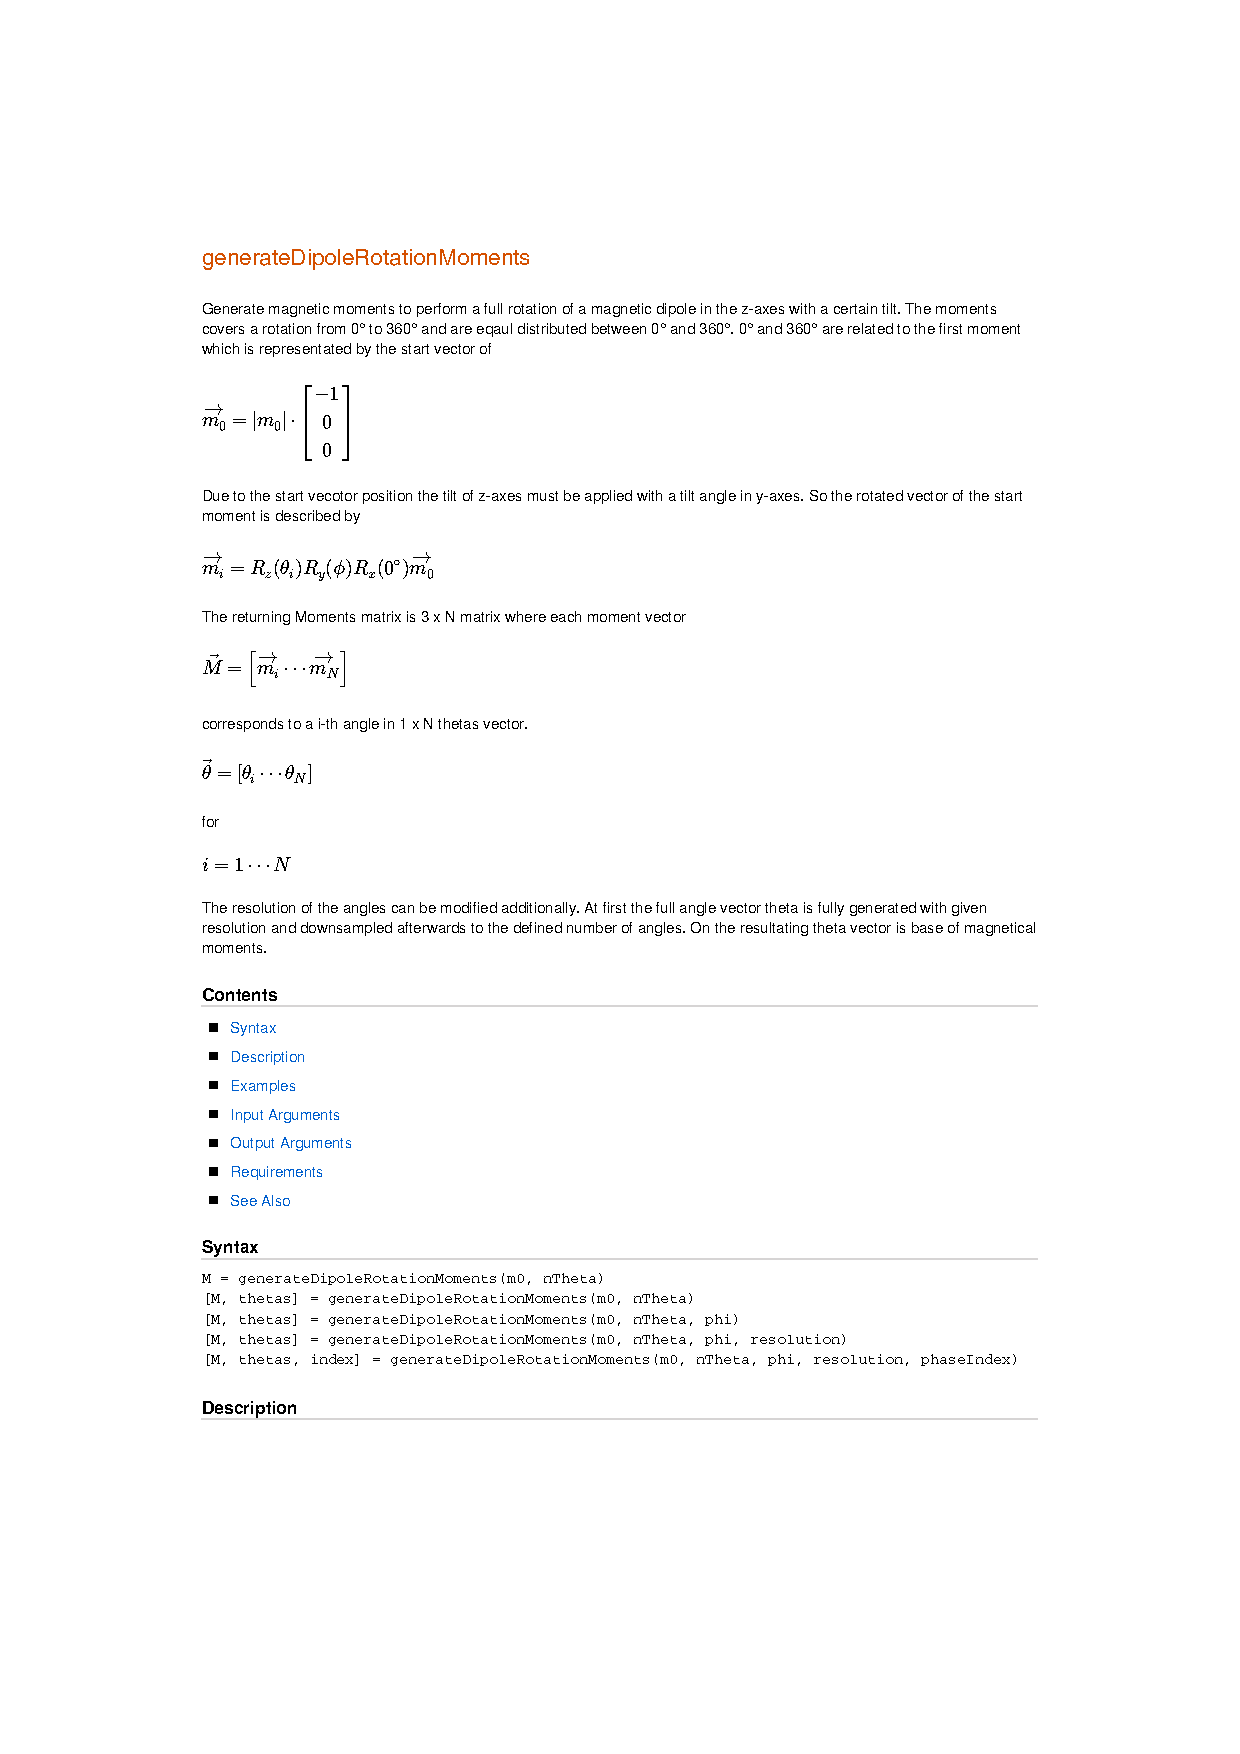
\includepdf[page=1,pagecommand={\phantomsection\addcontentsline{toc}{subsubsection}{\protect\numberline{\thesubsubsection}generateDipoleRotationMoments}\label{generateDipoleRotationMoments}}]{generateDipoleRotationMoments.pdf}
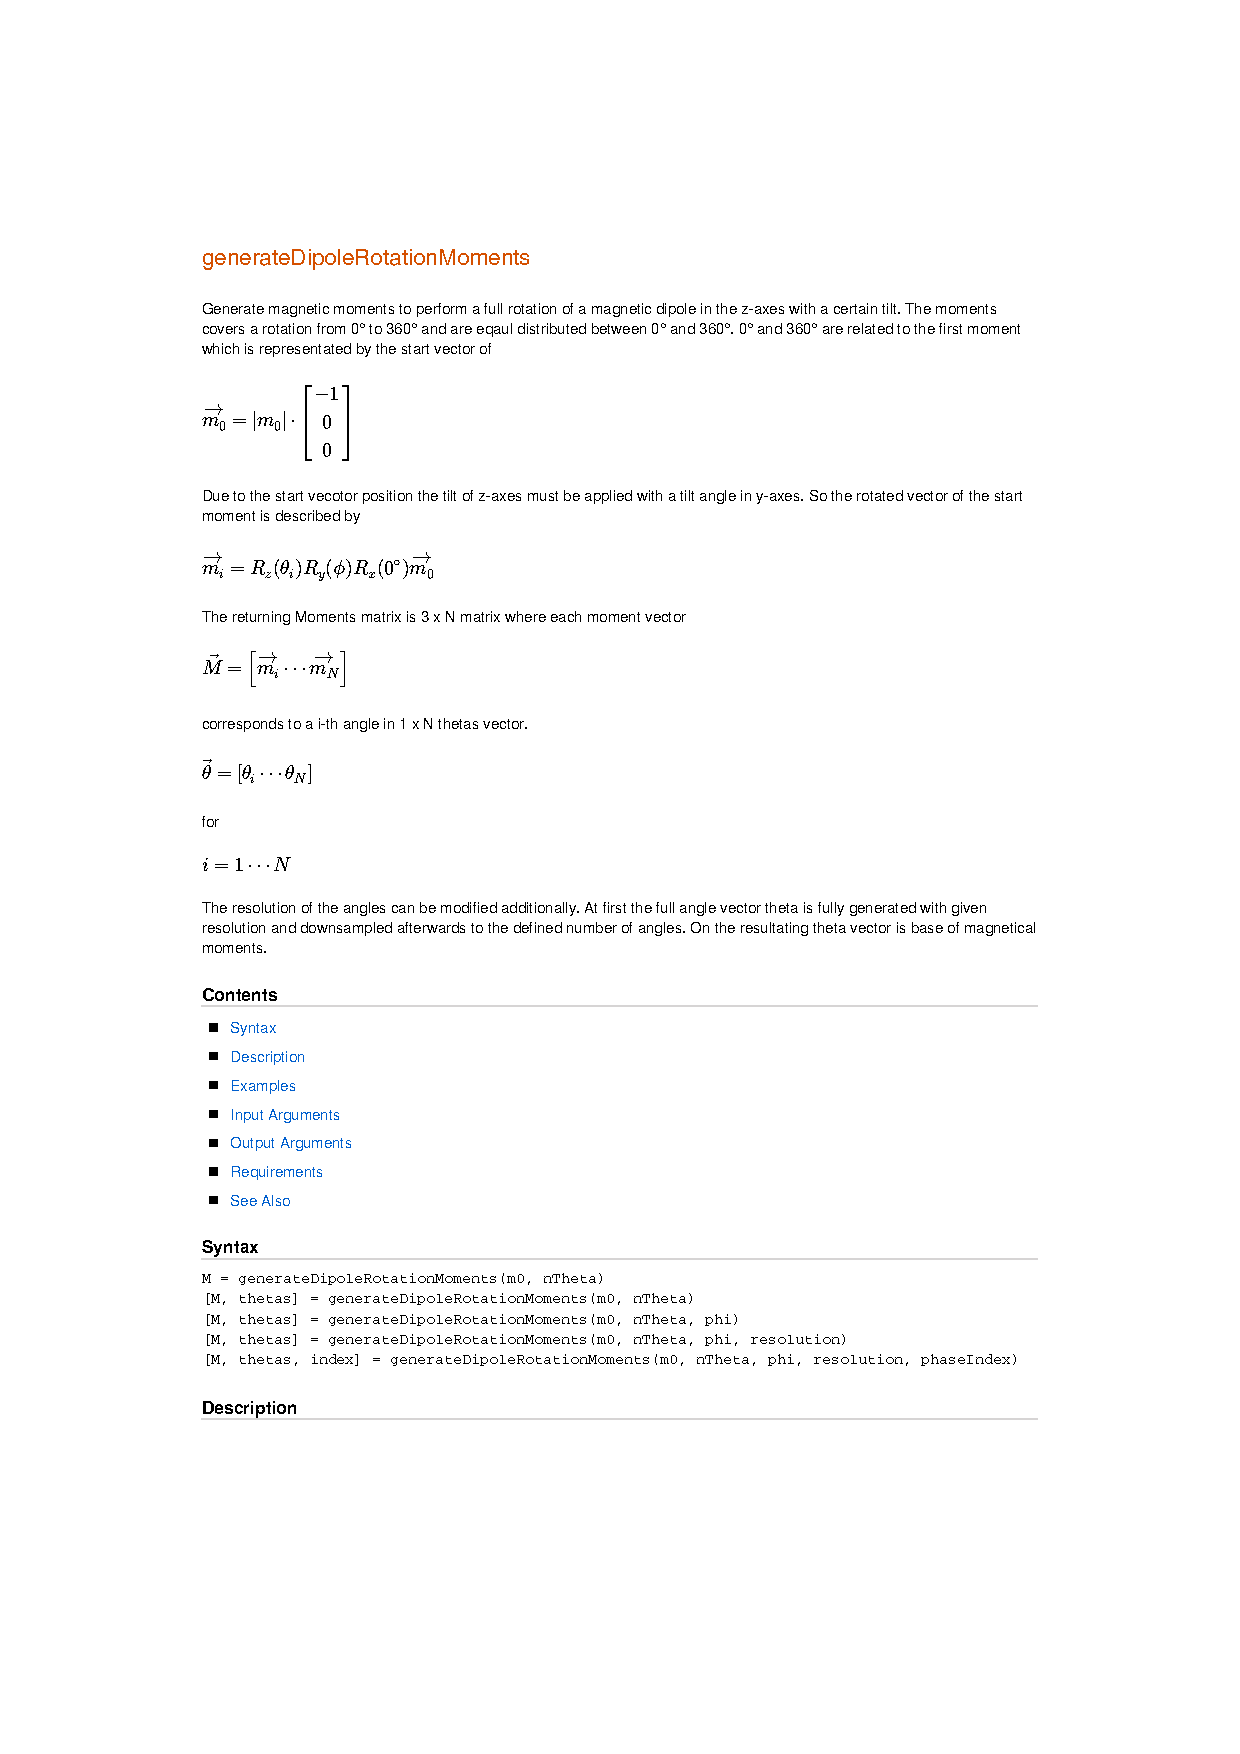
\includepdf[page=2-, pagecommand={\phantomsection}]{generateDipoleRotationMoments.pdf}
\addtocounter{subsubsection}{1}
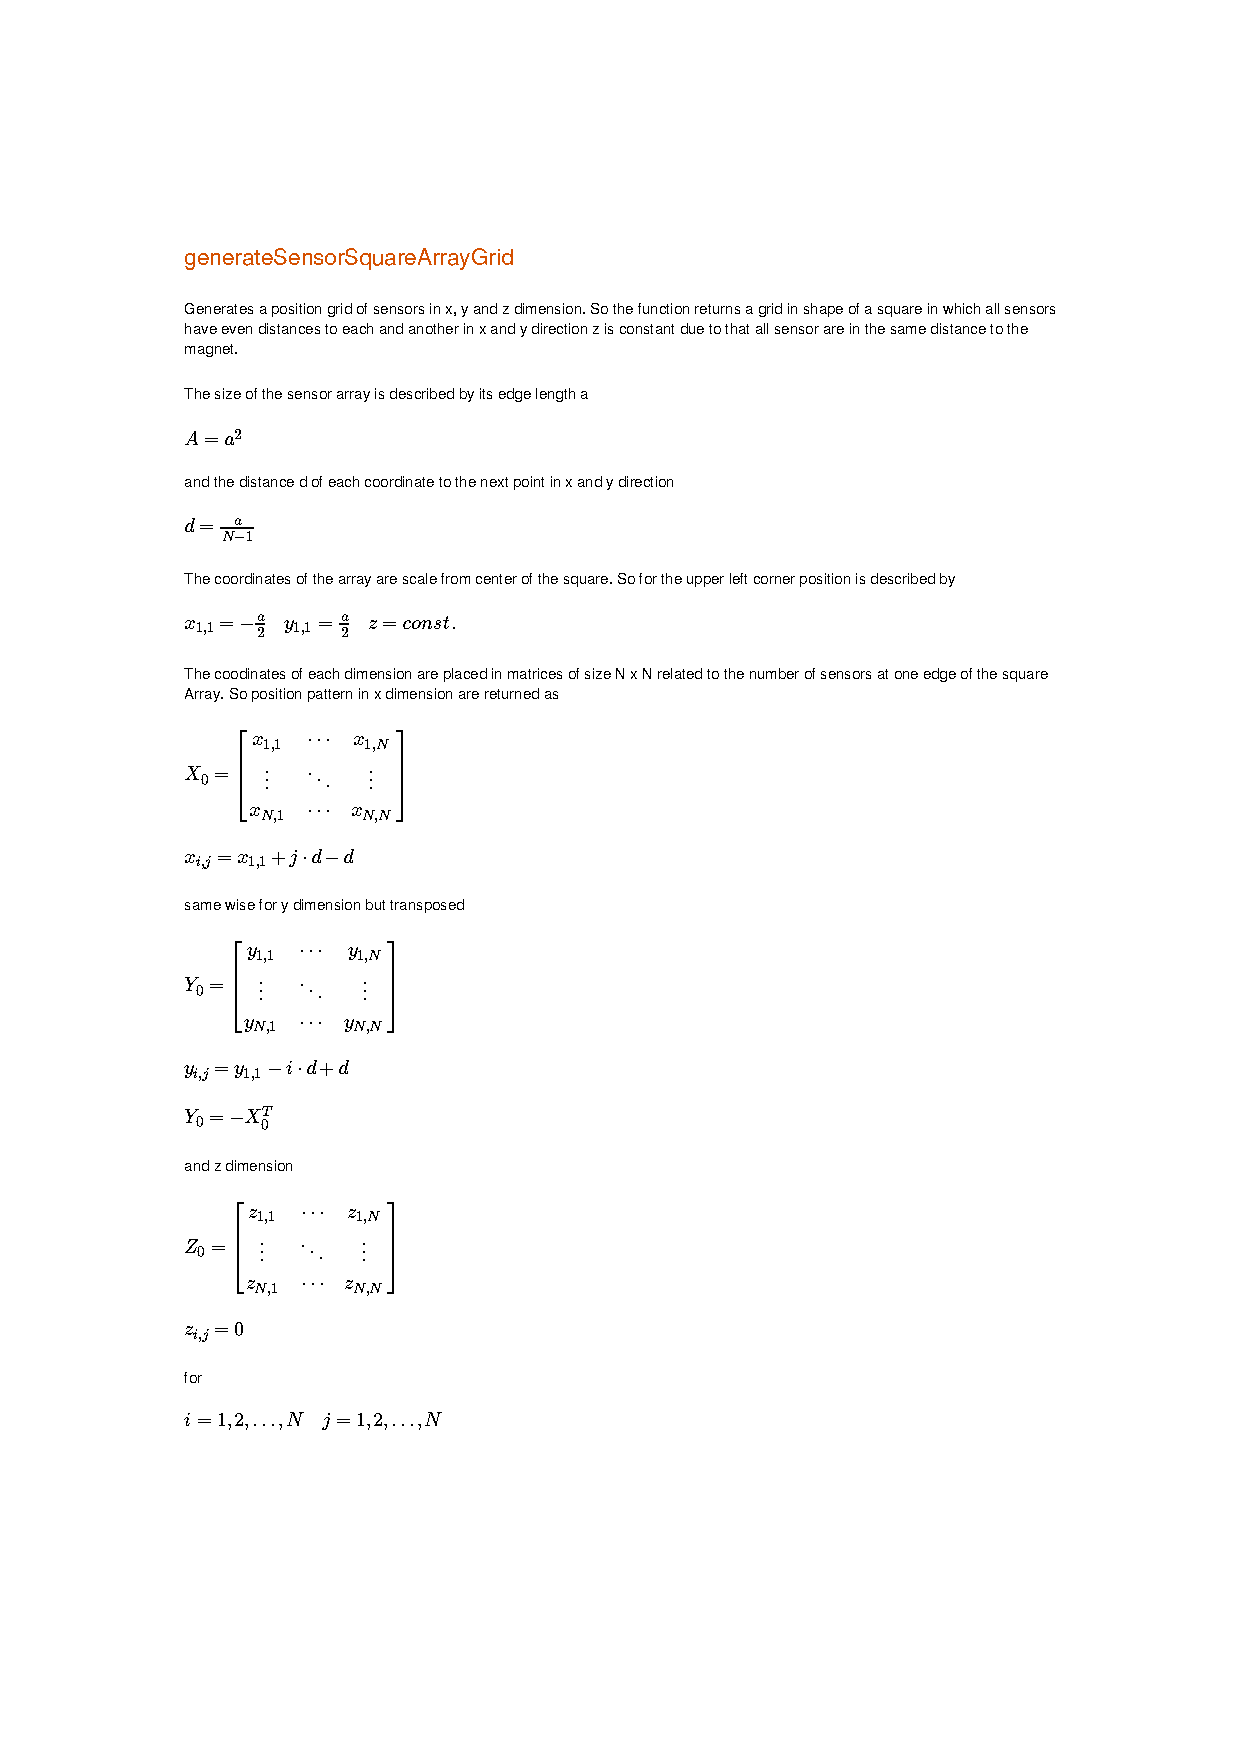
\includepdf[page=1,pagecommand={\phantomsection\addcontentsline{toc}{subsubsection}{\protect\numberline{\thesubsubsection}generateSensorArraySquareGrid}\label{generateSensorArraySquareGrid}}]{generateSensorArraySquareGrid.pdf}
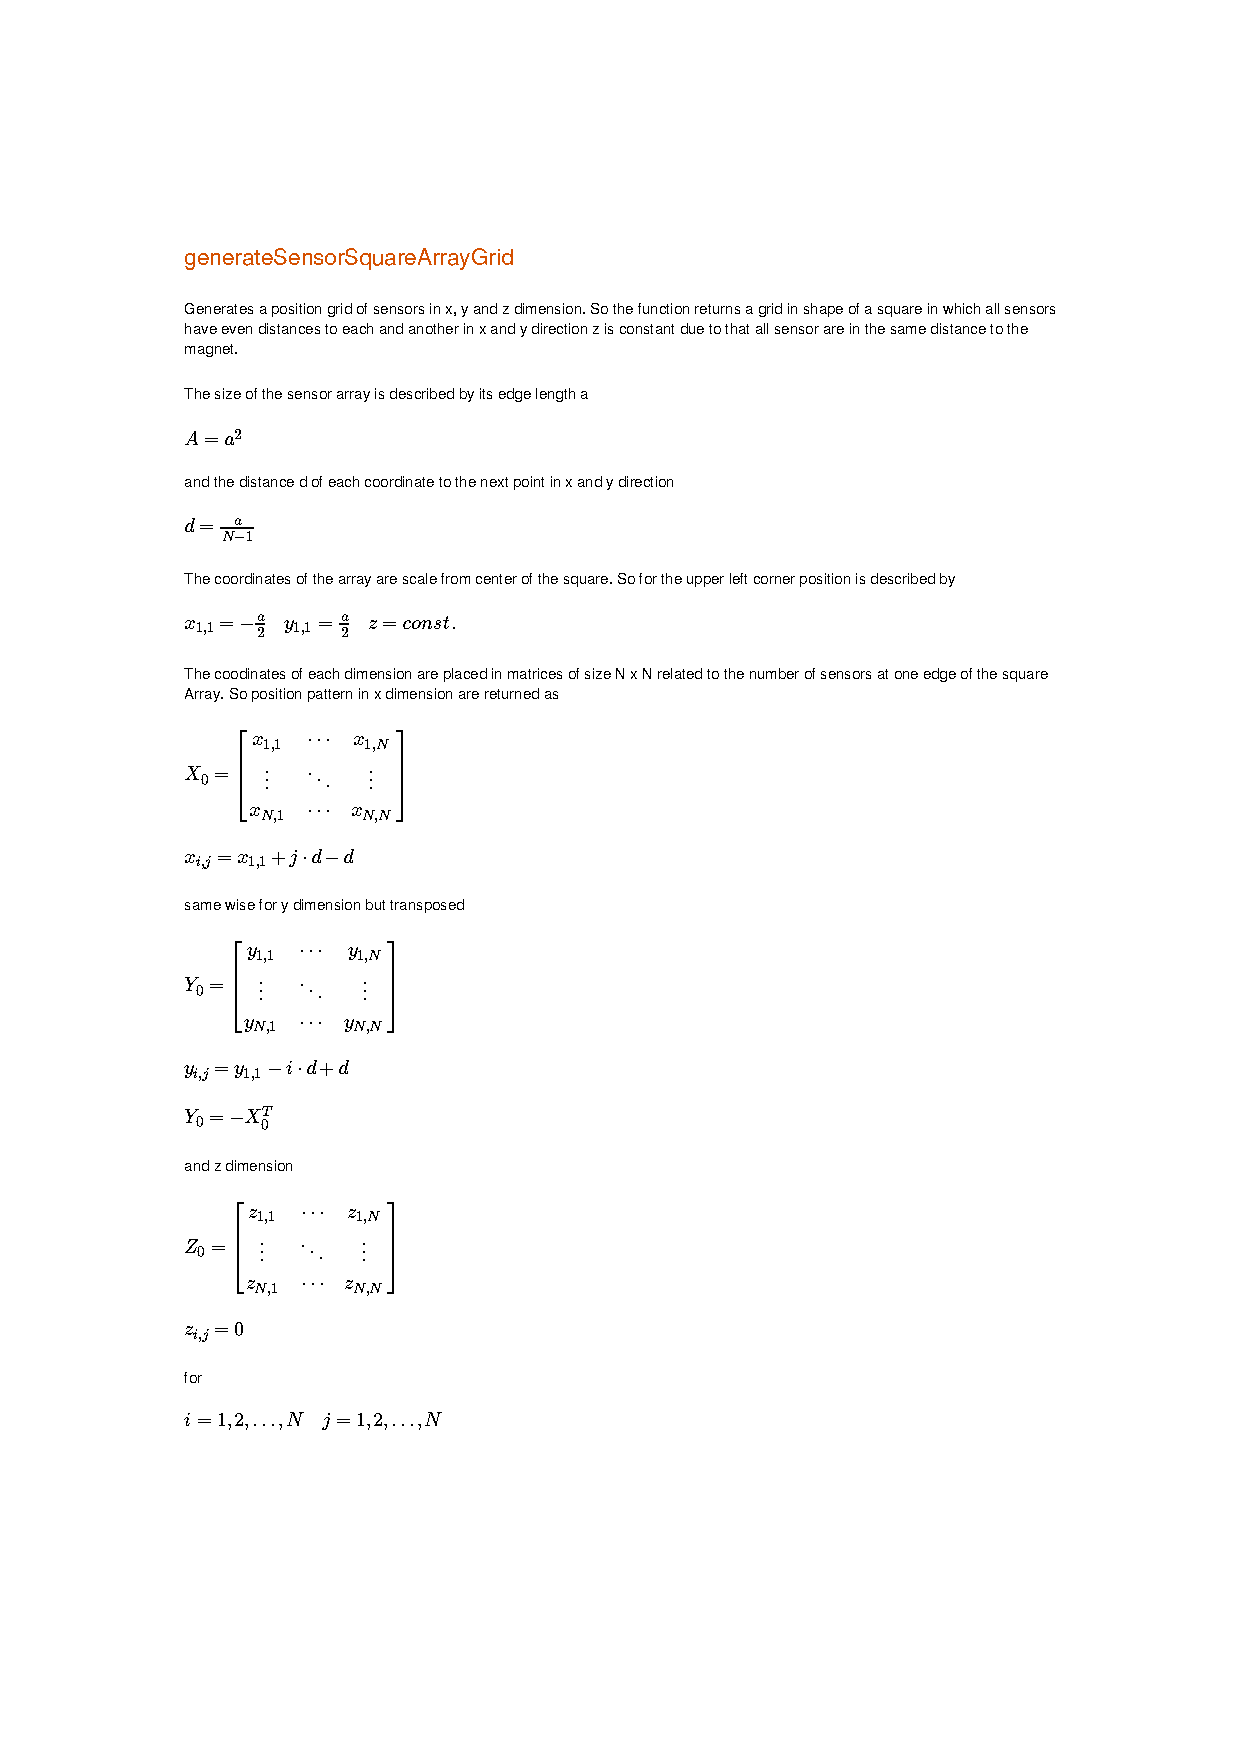
\includepdf[page=2-, pagecommand={\phantomsection}]{generateSensorArraySquareGrid.pdf}
\addtocounter{subsubsection}{1}
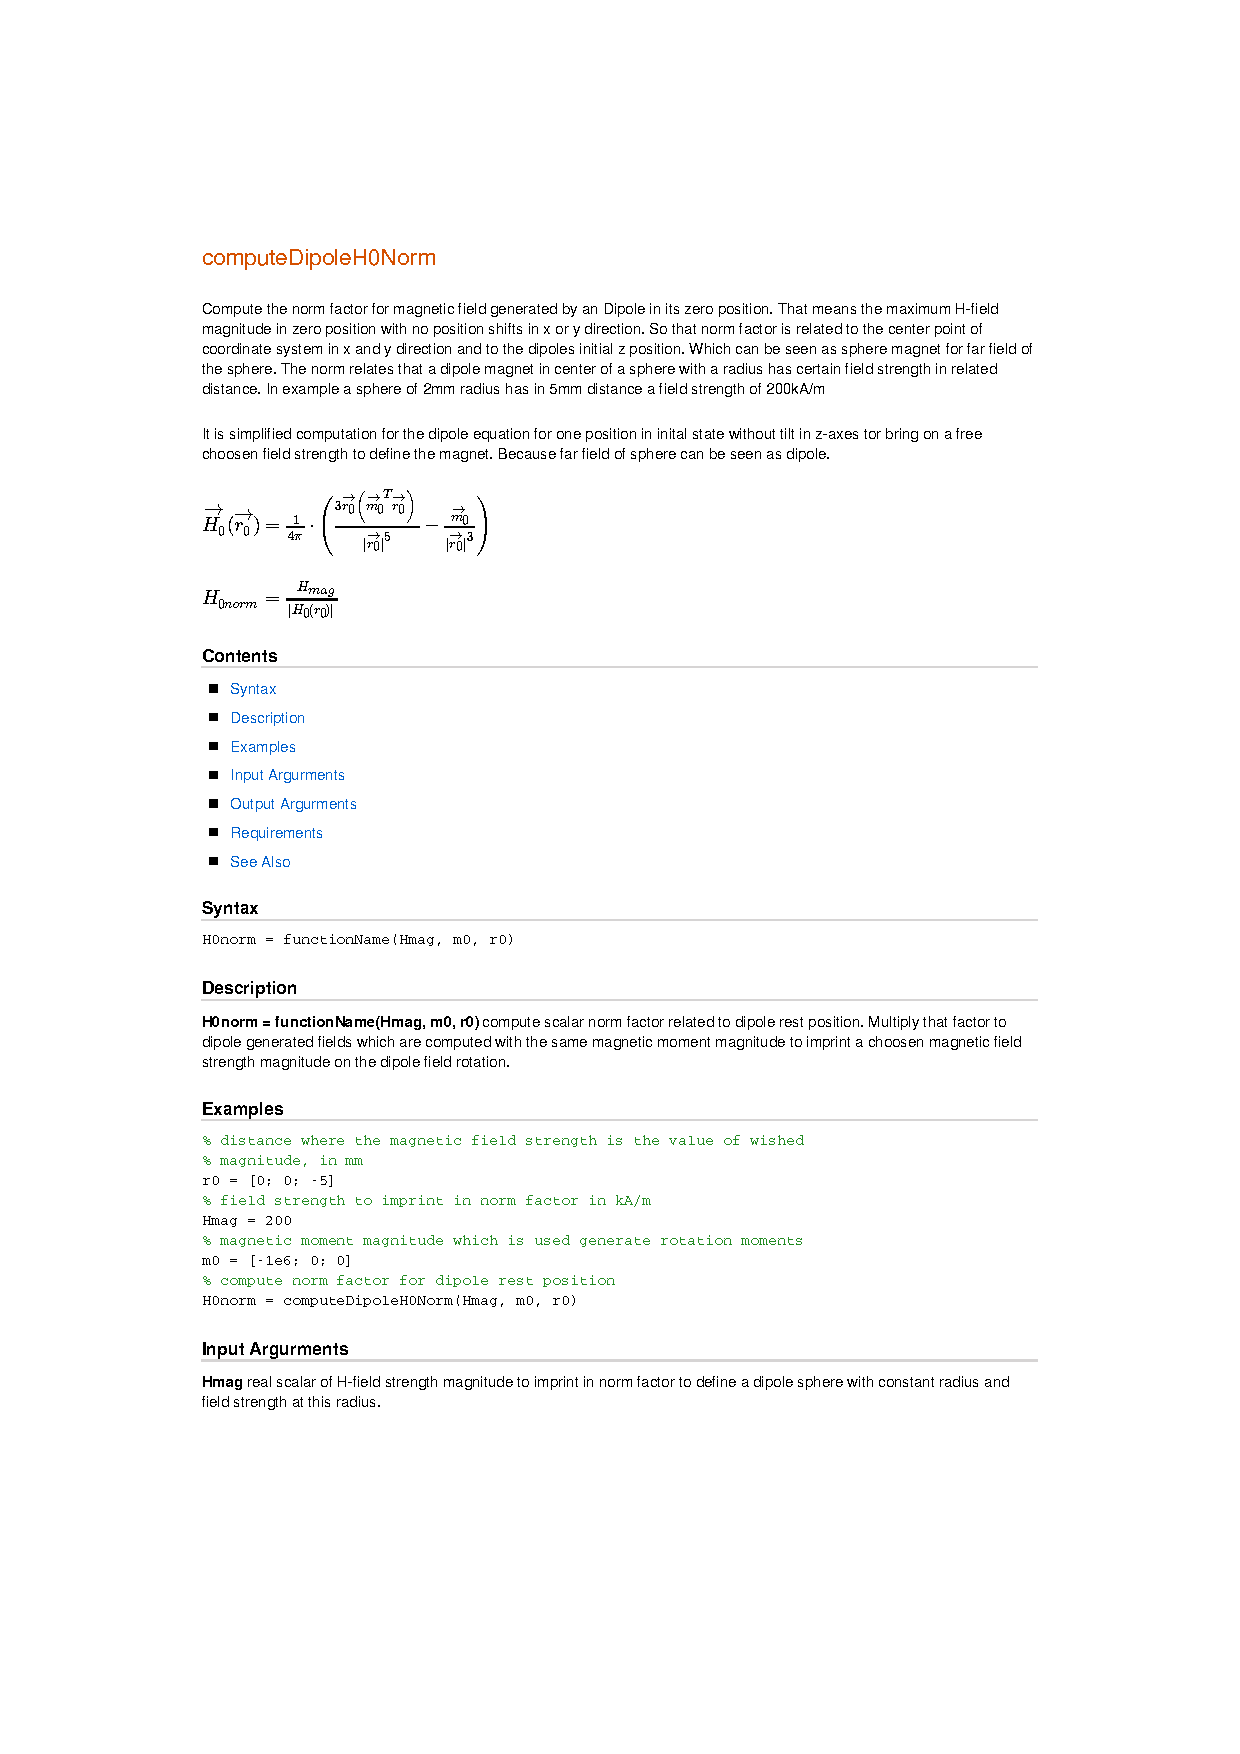
\includepdf[page=1,pagecommand={\phantomsection\addcontentsline{toc}{subsubsection}{\protect\numberline{\thesubsubsection}computeDipoleH0Norm}\label{computeDipoleH0Norm}}]{computeDipoleH0Norm.pdf}
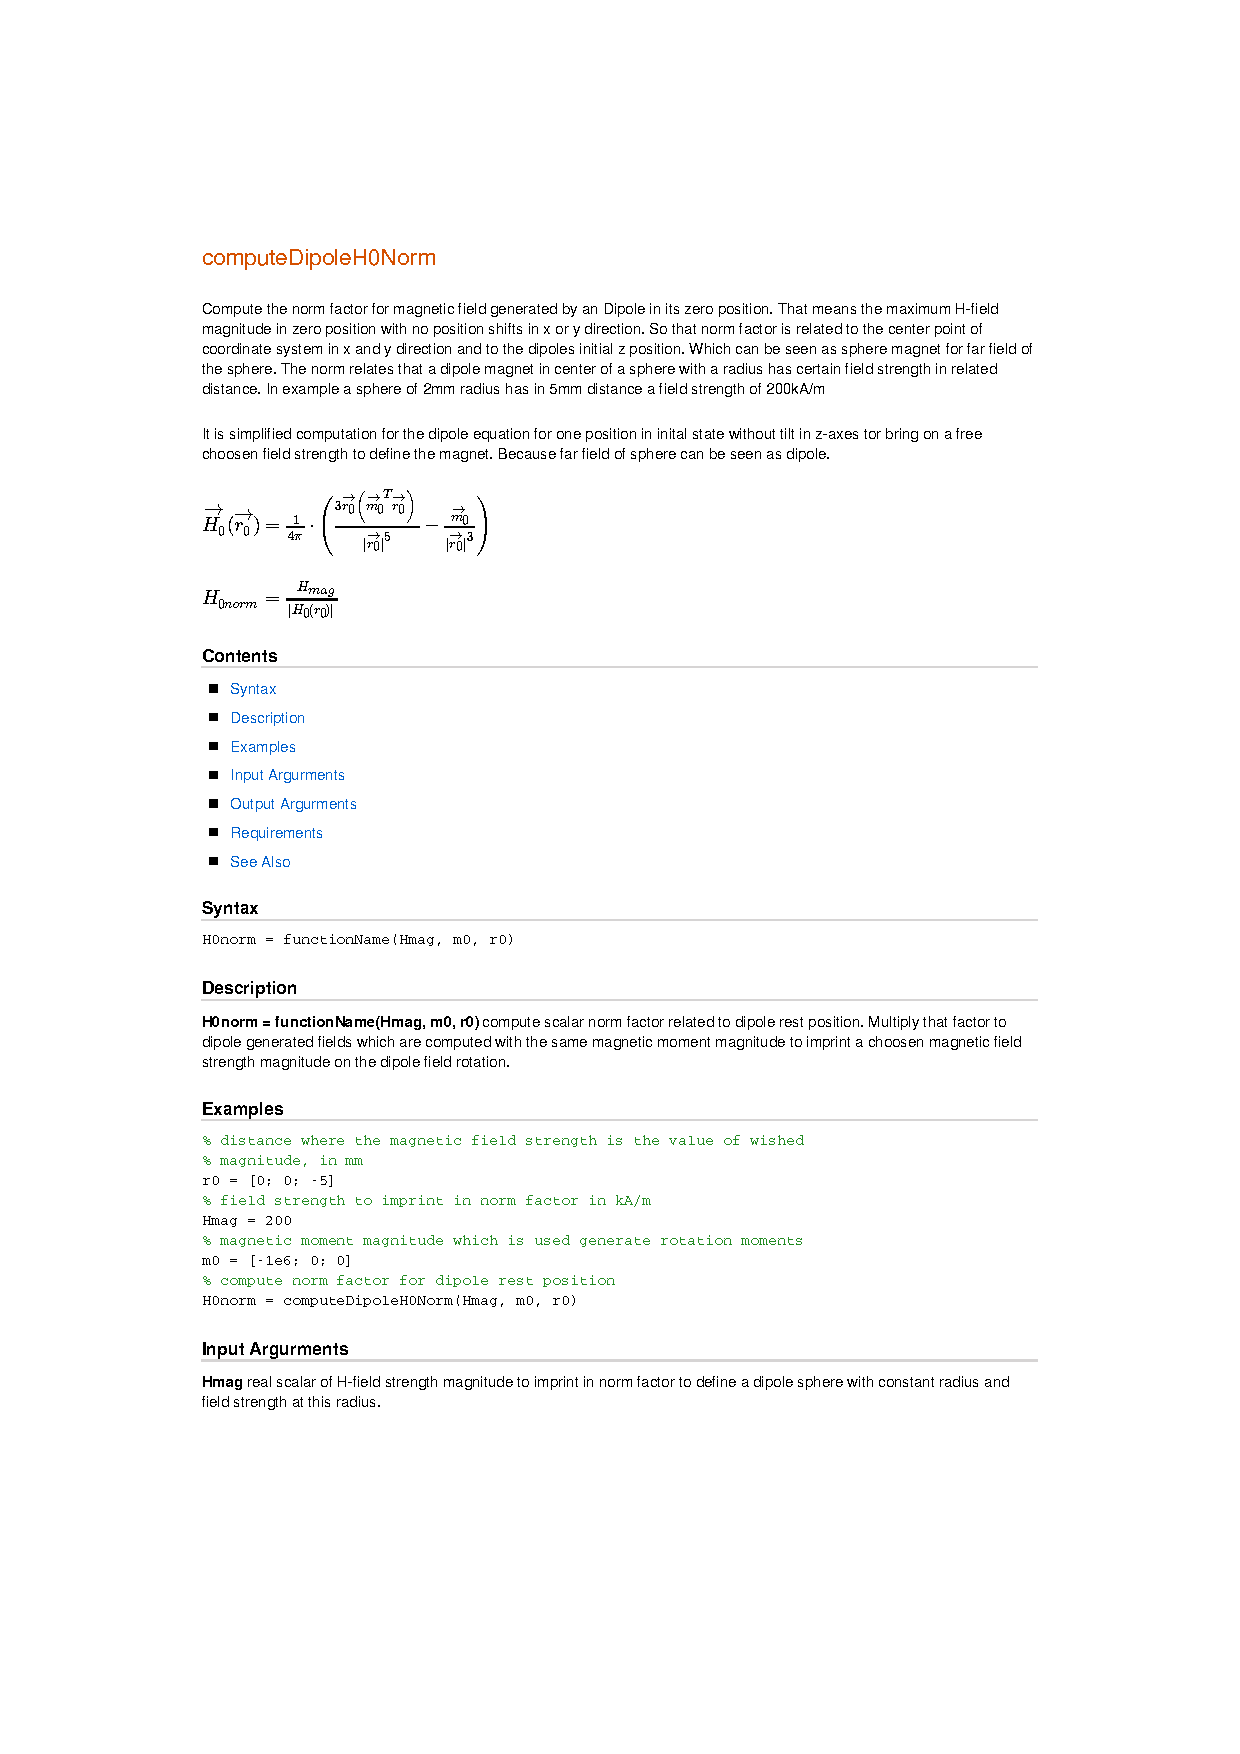
\includepdf[page=2-, pagecommand={\phantomsection}]{computeDipoleH0Norm.pdf}
\addtocounter{subsubsection}{1}
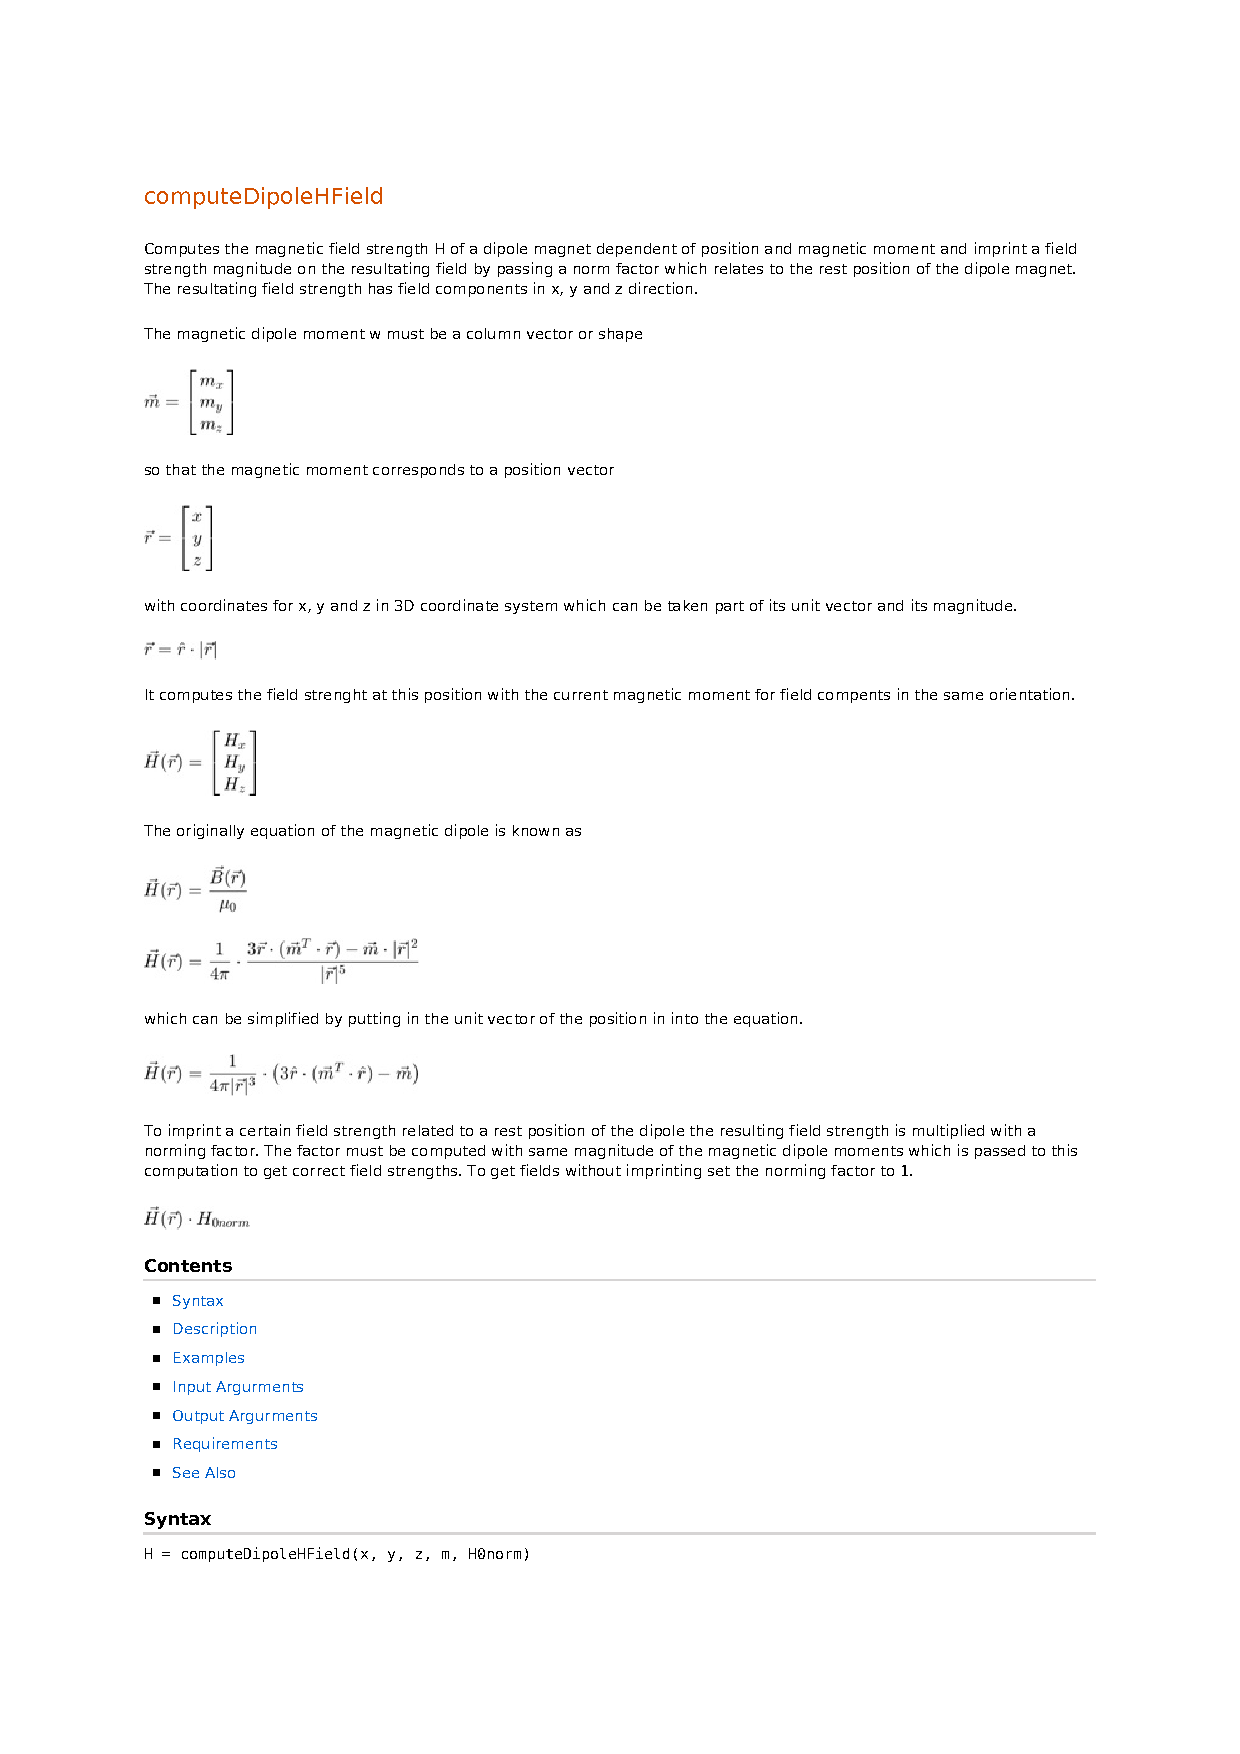
\includepdf[page=1,pagecommand={\phantomsection\addcontentsline{toc}{subsubsection}{\protect\numberline{\thesubsubsection}computeDipoleHField}\label{computeDipoleHField}}]{computeDipoleHField.pdf}
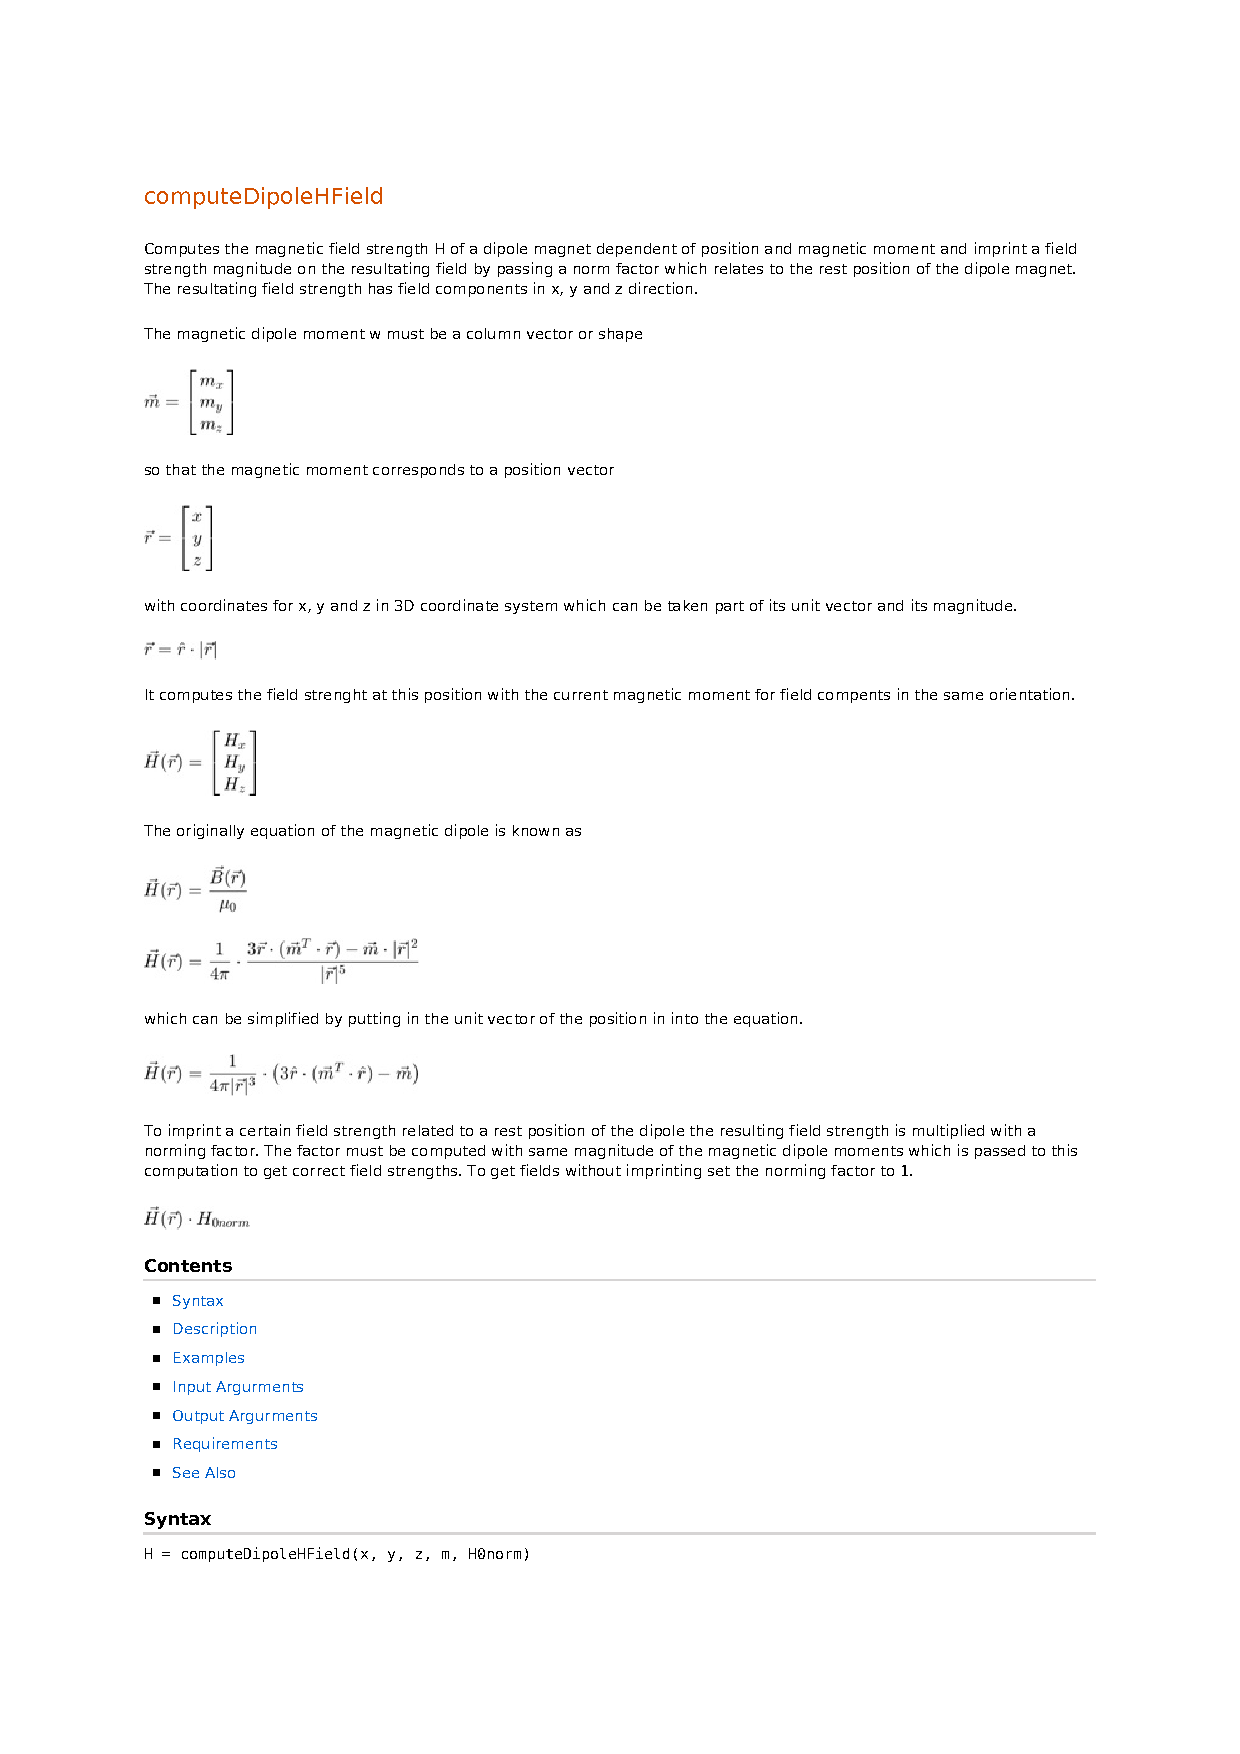
\includepdf[page=2-, pagecommand={\phantomsection}]{computeDipoleHField.pdf}
\addtocounter{subsubsection}{1}
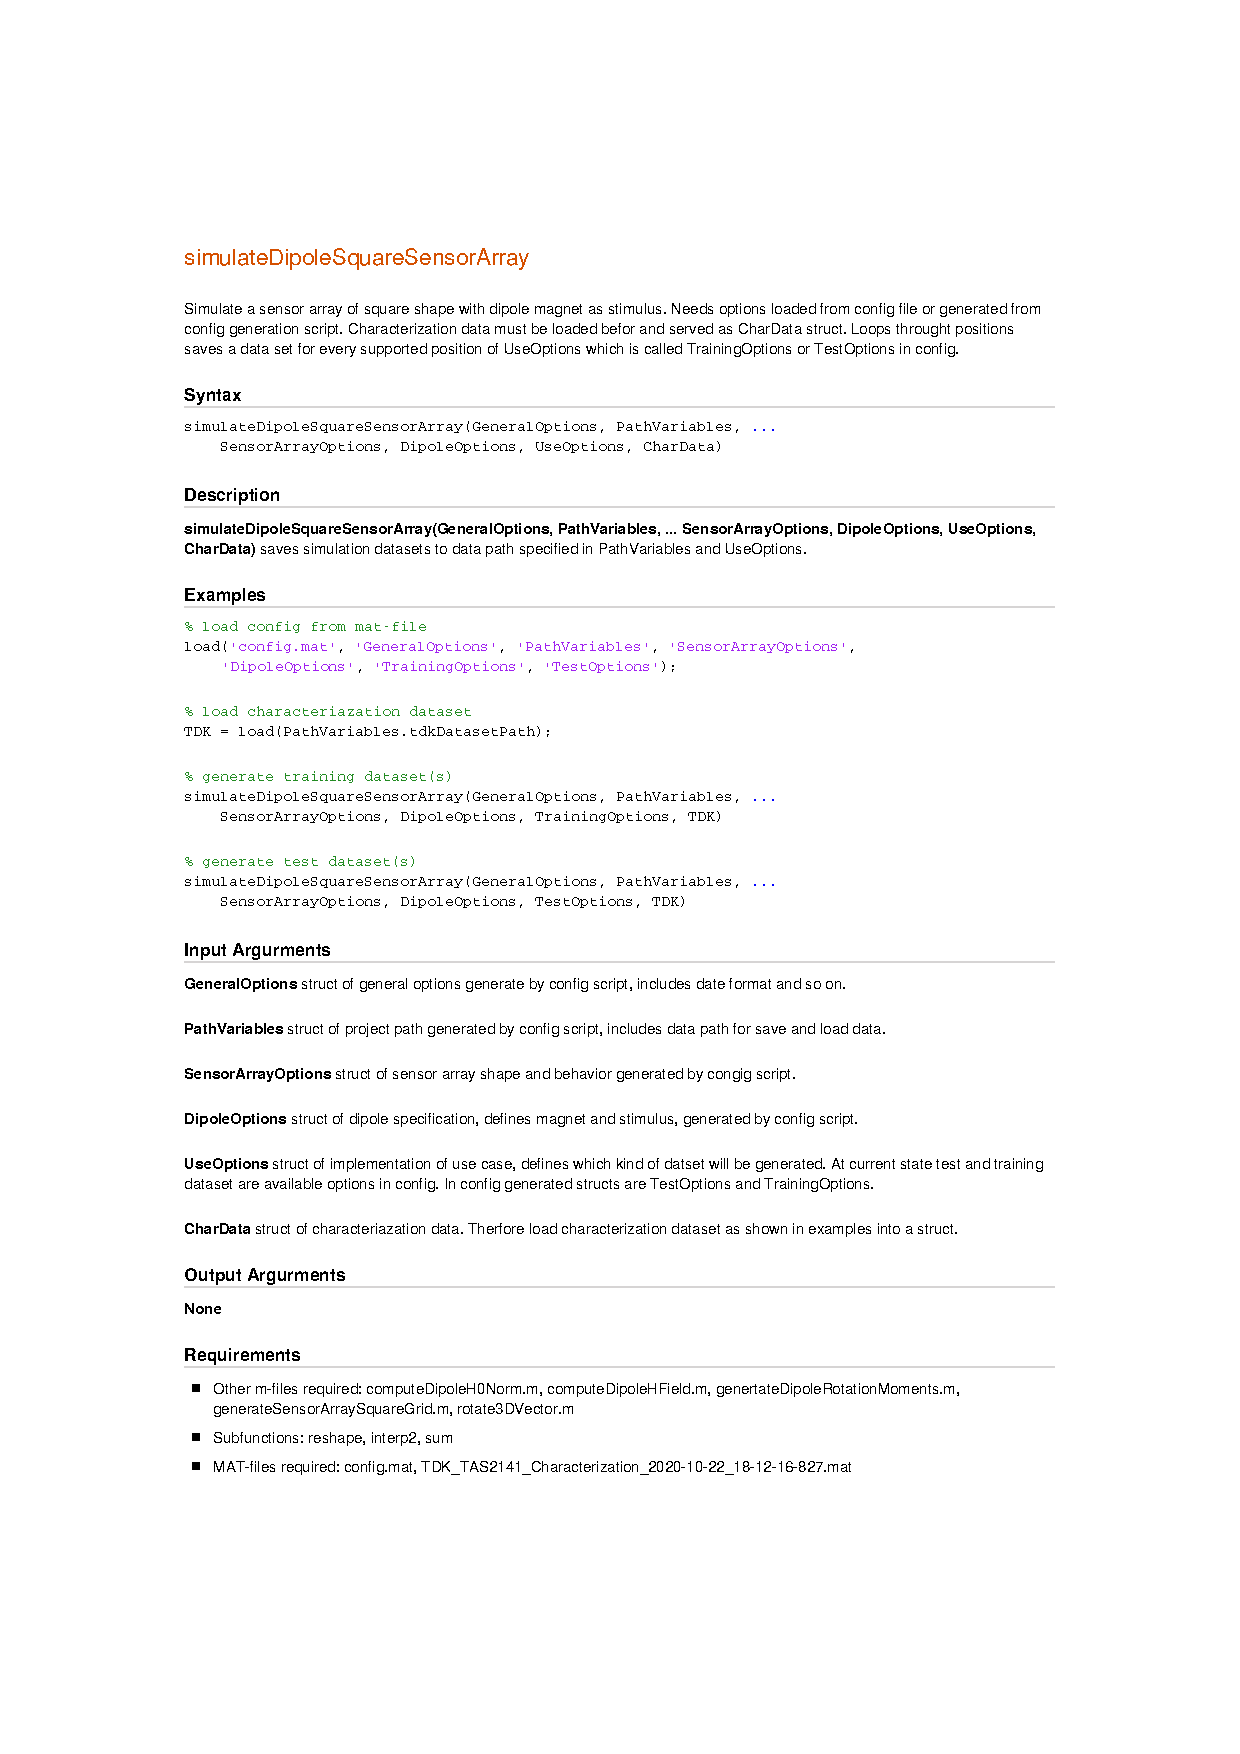
\includepdf[page=1,pagecommand={\phantomsection\addcontentsline{toc}{subsubsection}{\protect\numberline{\thesubsubsection}simulateDipoleSquareSensorArray}\label{simulateDipoleSquareSensorArray}}]{simulateDipoleSquareSensorArray.pdf}
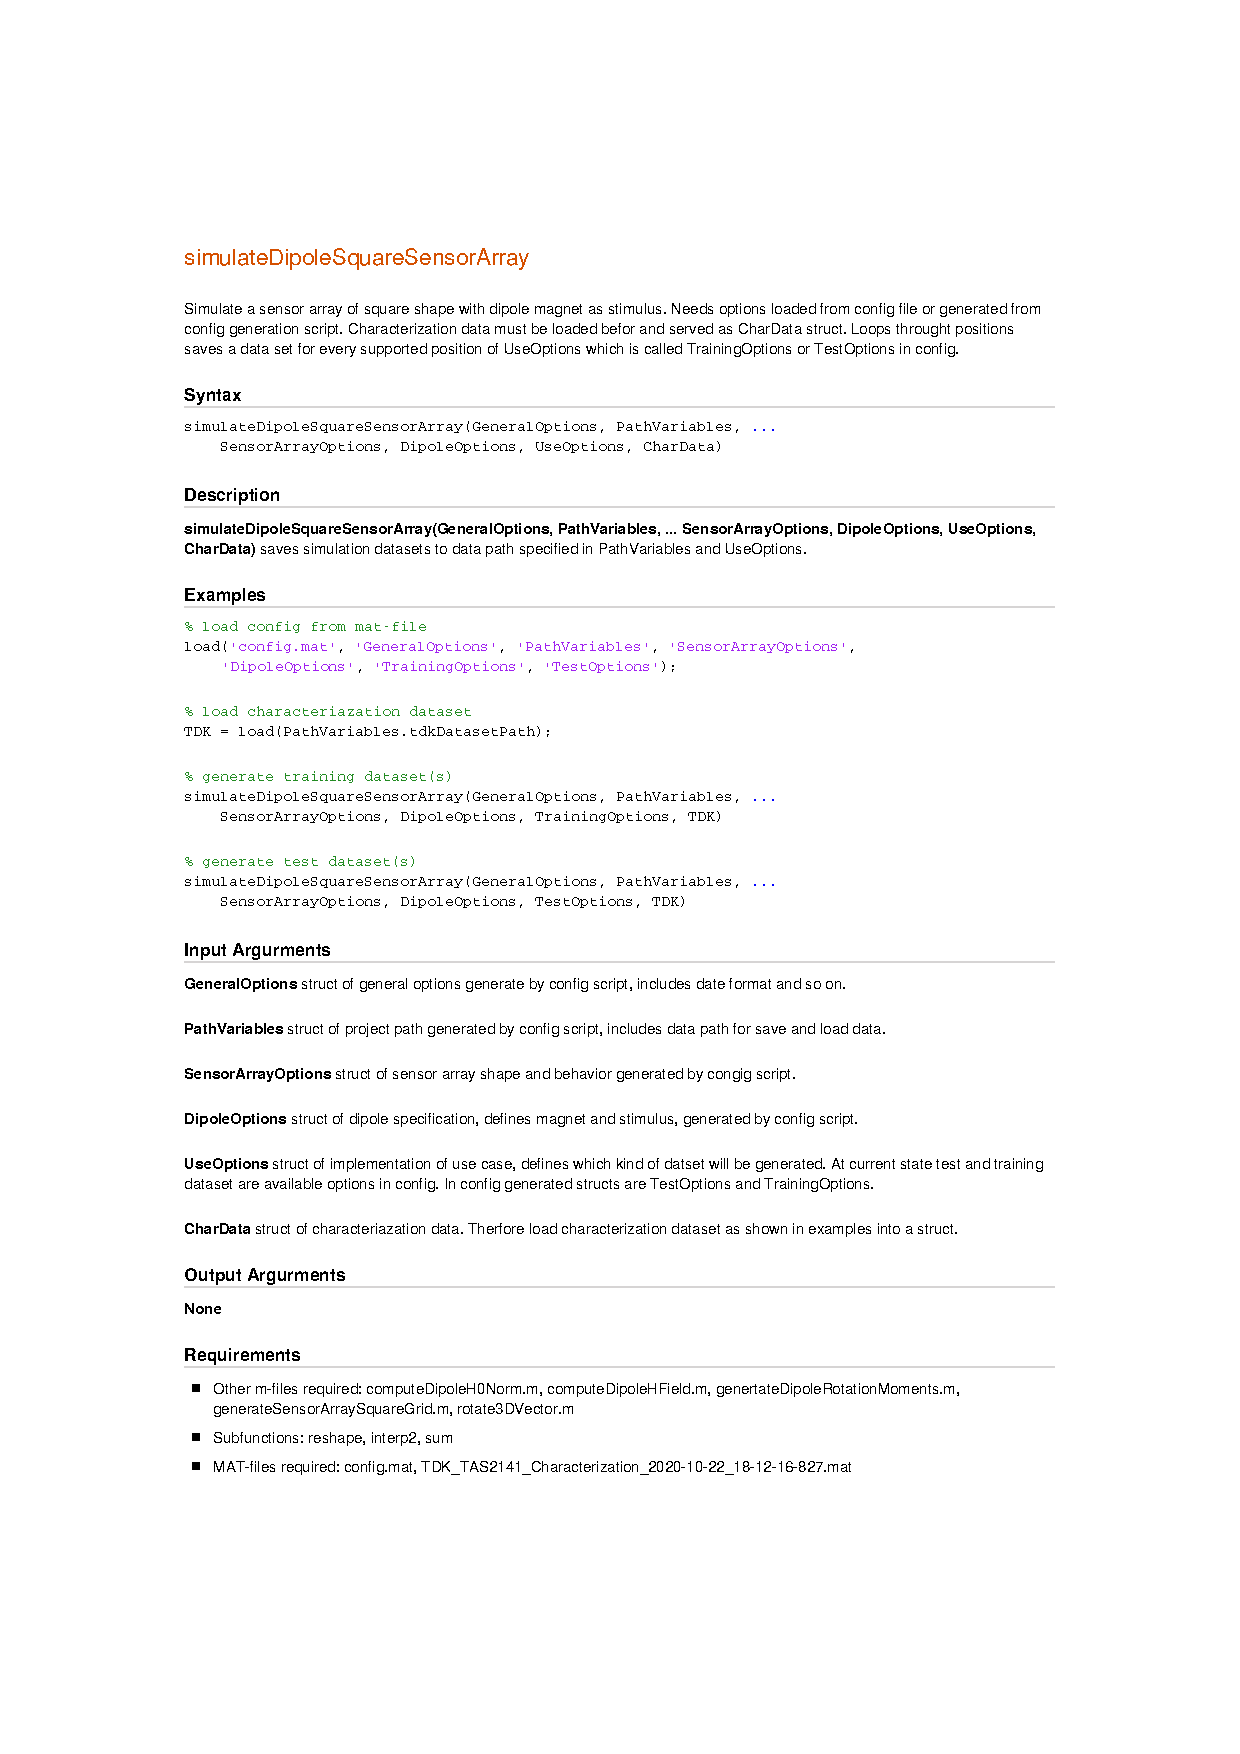
\includepdf[page=2-, pagecommand={\phantomsection}]{simulateDipoleSquareSensorArray.pdf}
\addtocounter{subsection}{1}
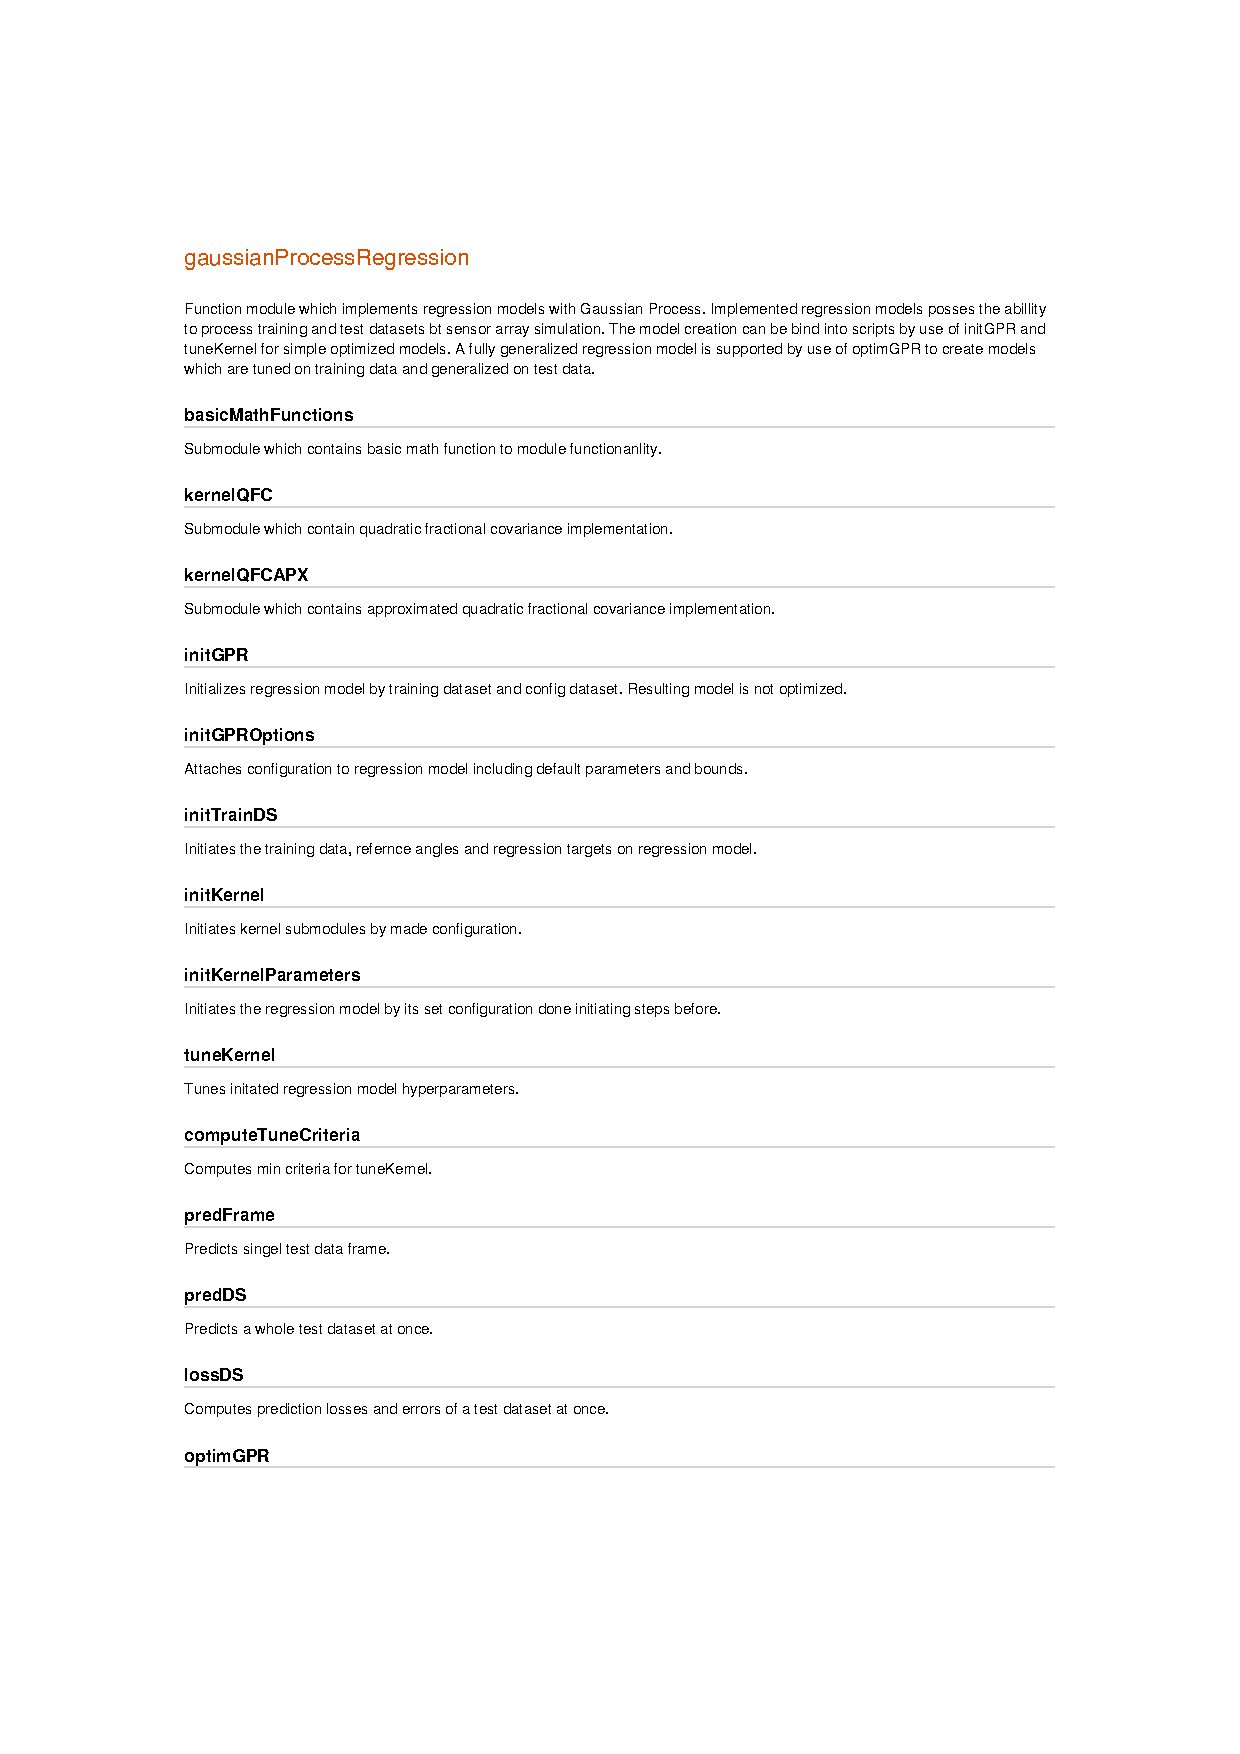
\includepdf[page=1,pagecommand={\phantomsection\addcontentsline{toc}{subsection}{\protect\numberline{\thesubsection}gaussianProcessRegression}\label{gaussianProcessRegression}}]{gaussianProcessRegression.pdf}
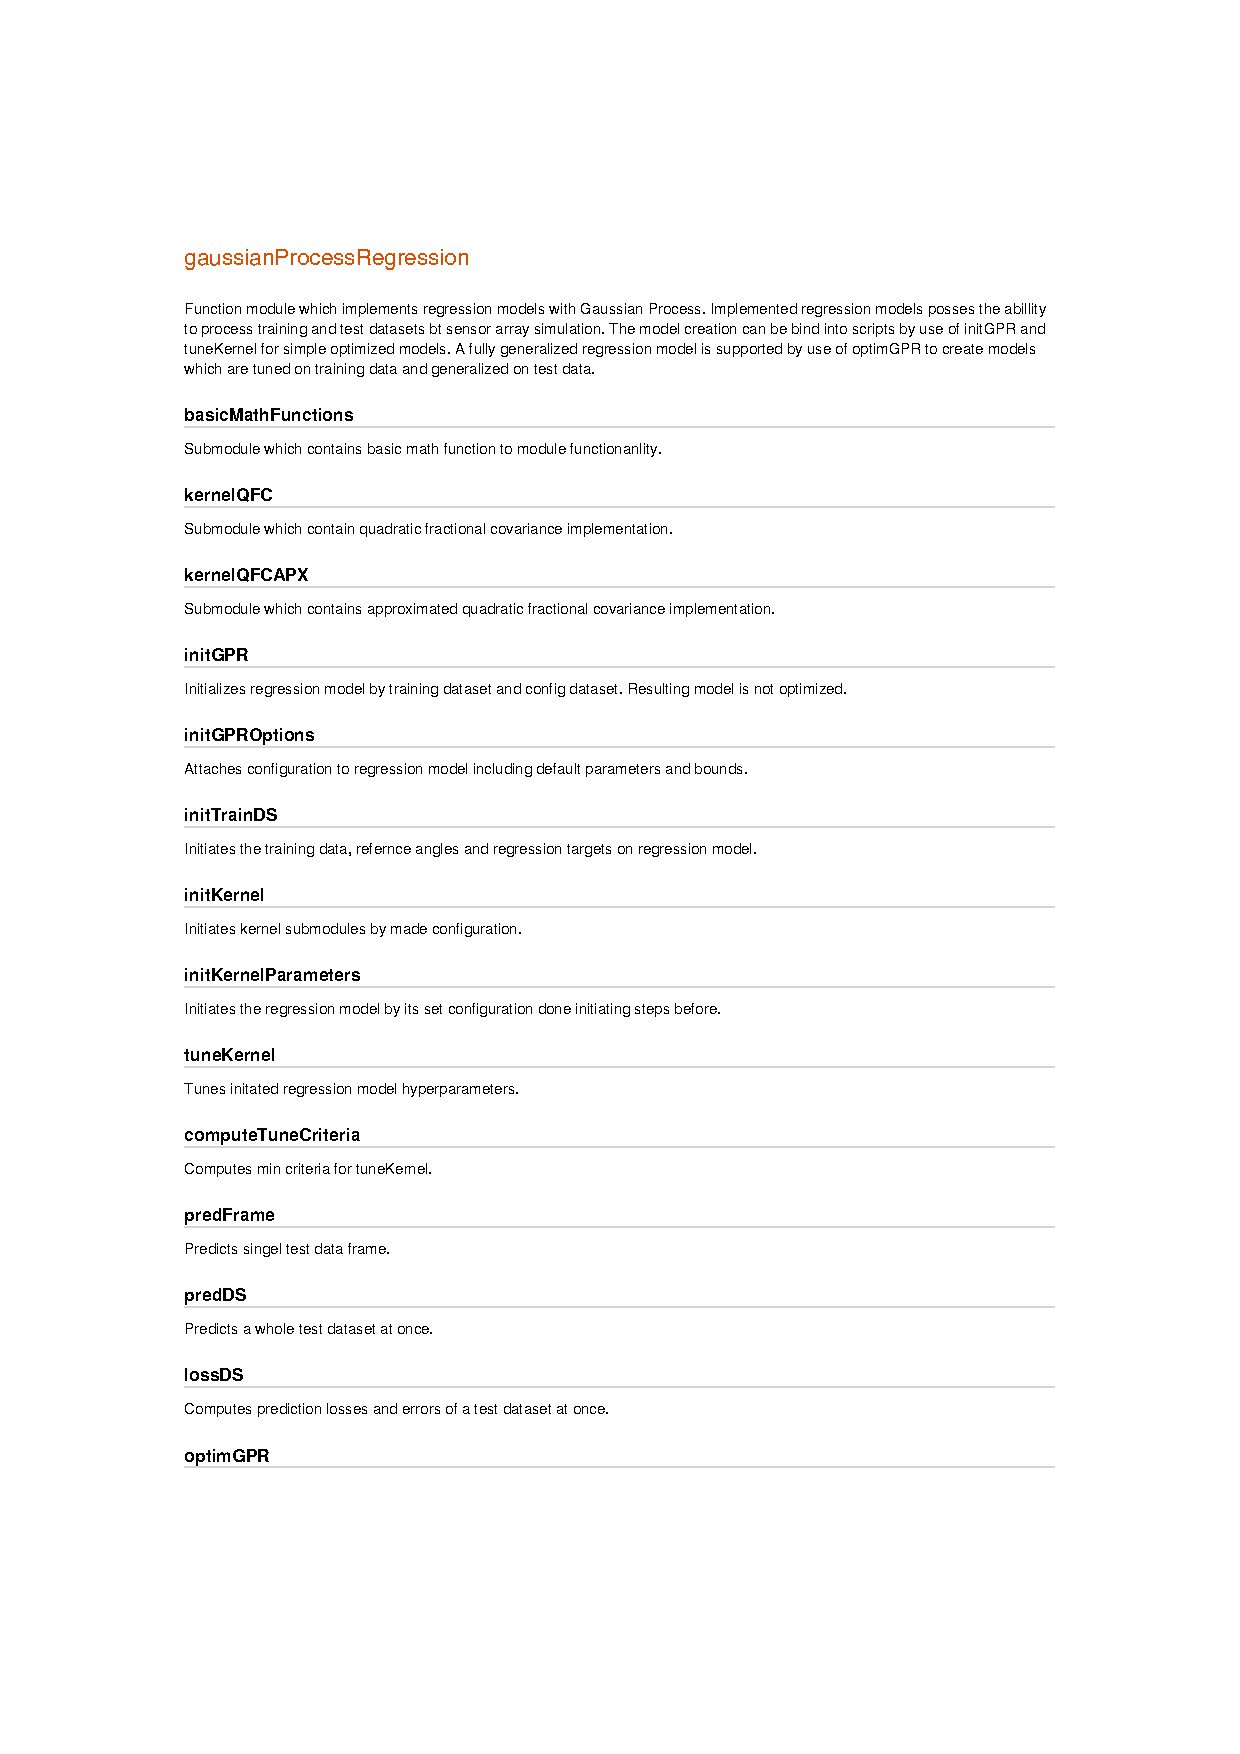
\includepdf[page=2-, pagecommand={\phantomsection}]{gaussianProcessRegression.pdf}
\addtocounter{subsubsection}{1}
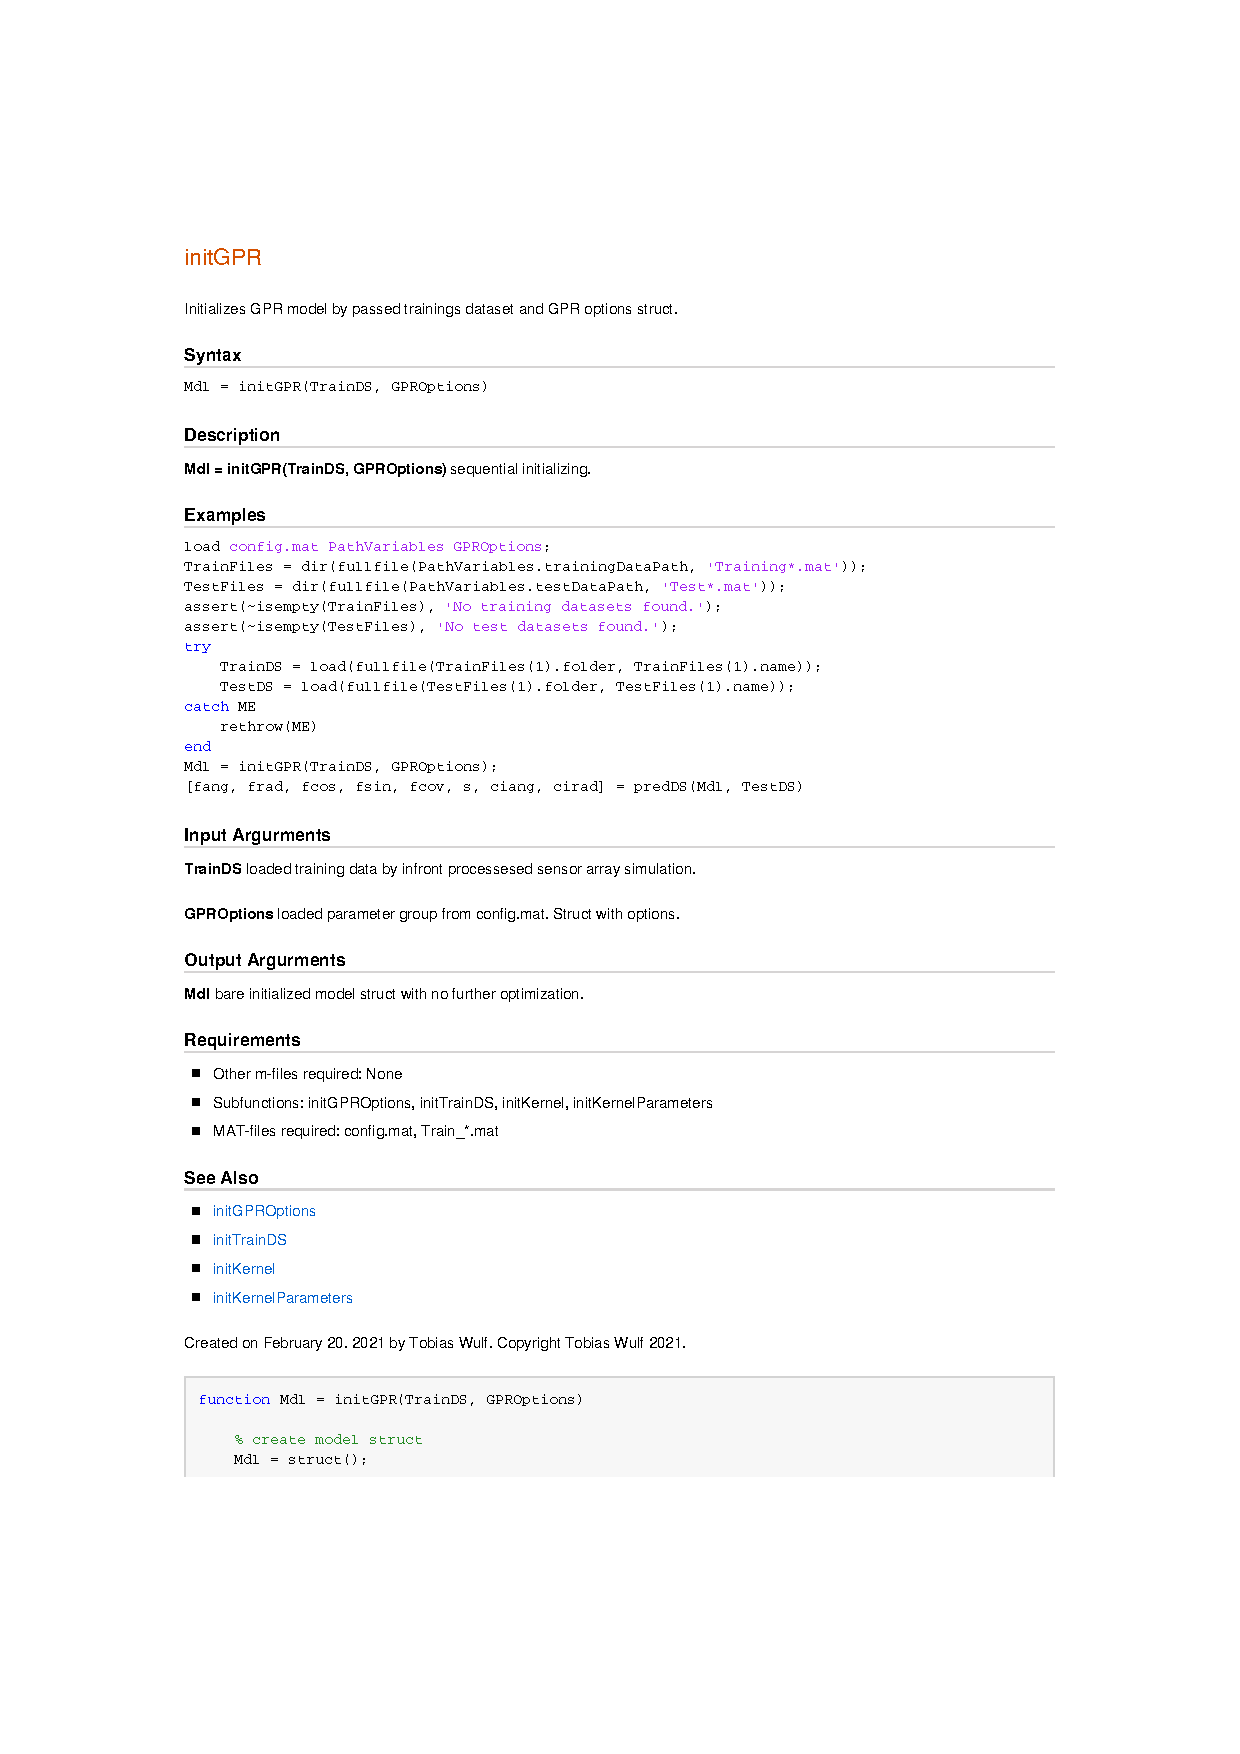
\includepdf[page=1,pagecommand={\phantomsection\addcontentsline{toc}{subsubsection}{\protect\numberline{\thesubsubsection}initGPR}\label{initGPR}}]{initGPR.pdf}
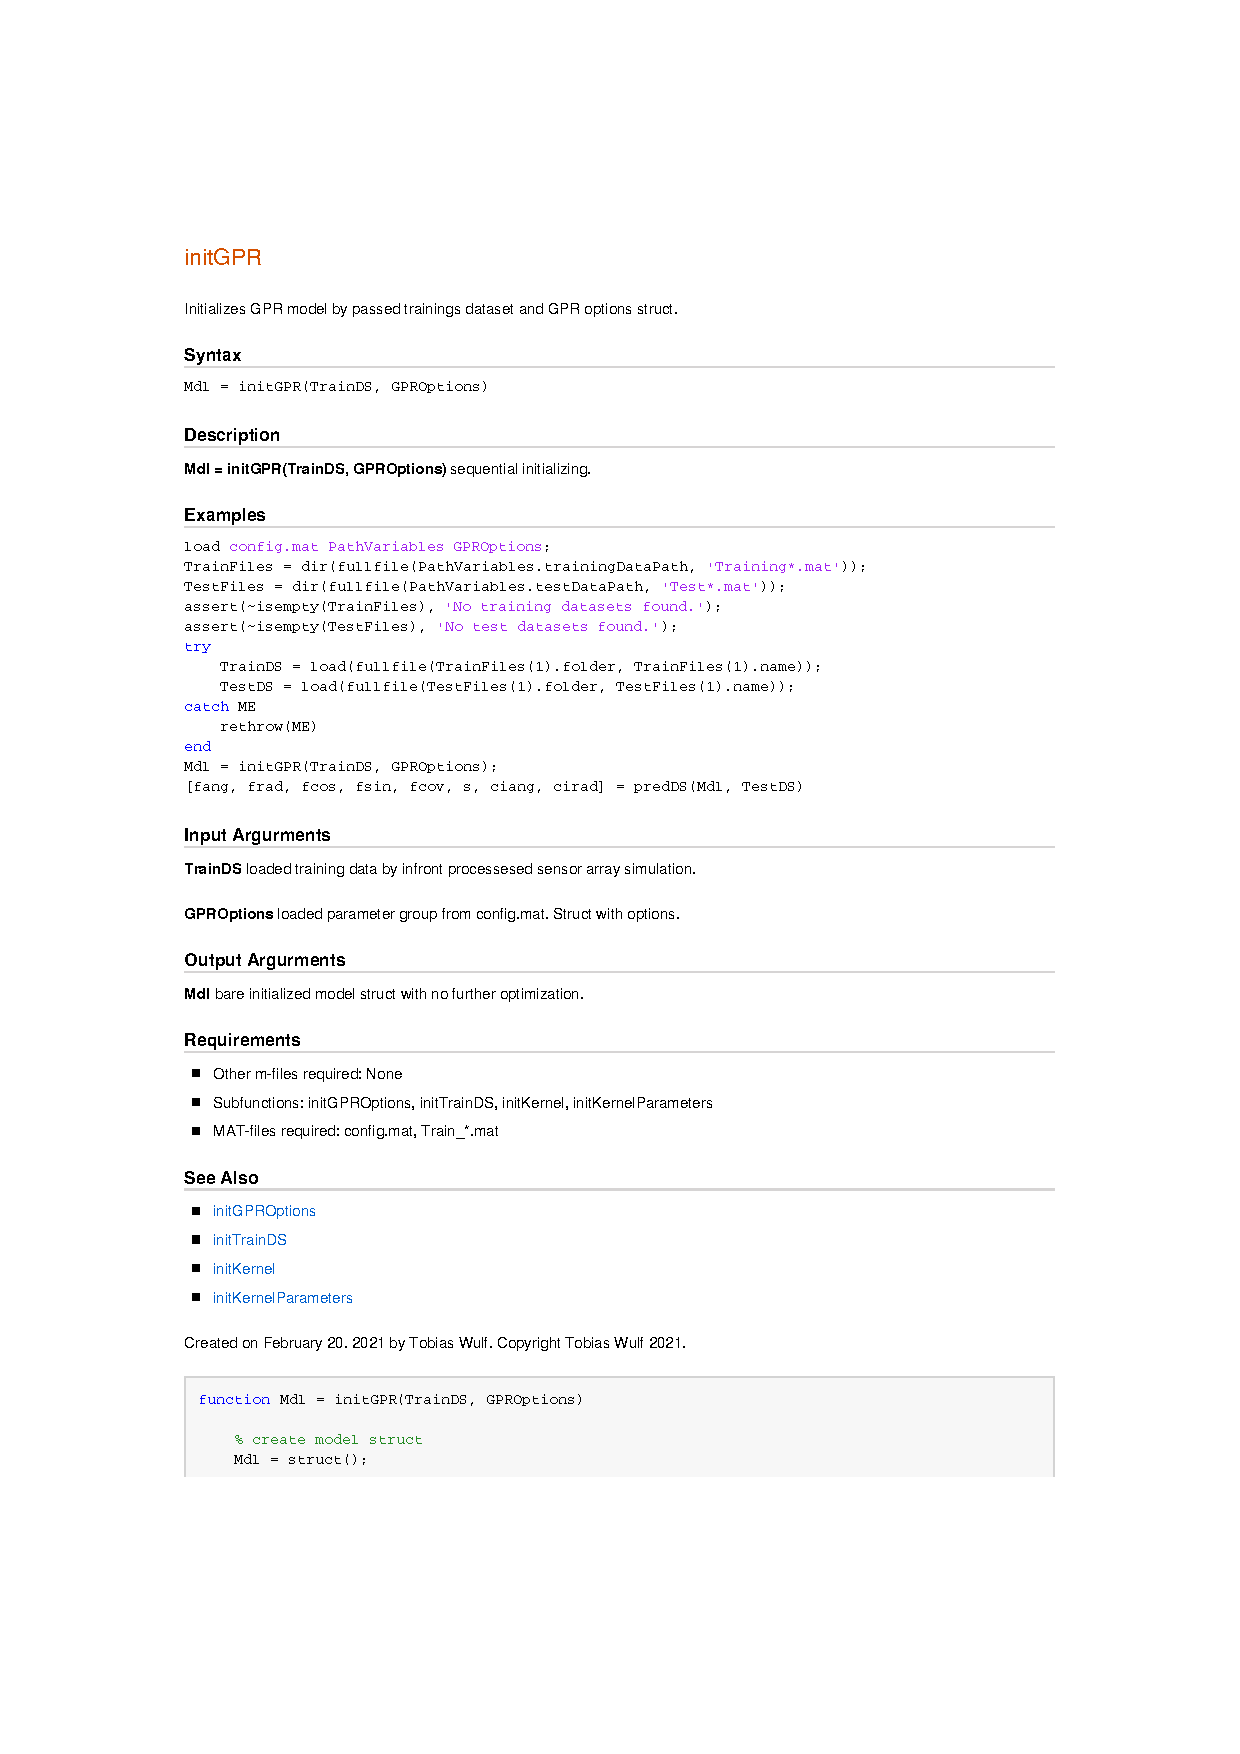
\includepdf[page=2-, pagecommand={\phantomsection}]{initGPR.pdf}
\addtocounter{subsubsection}{1}
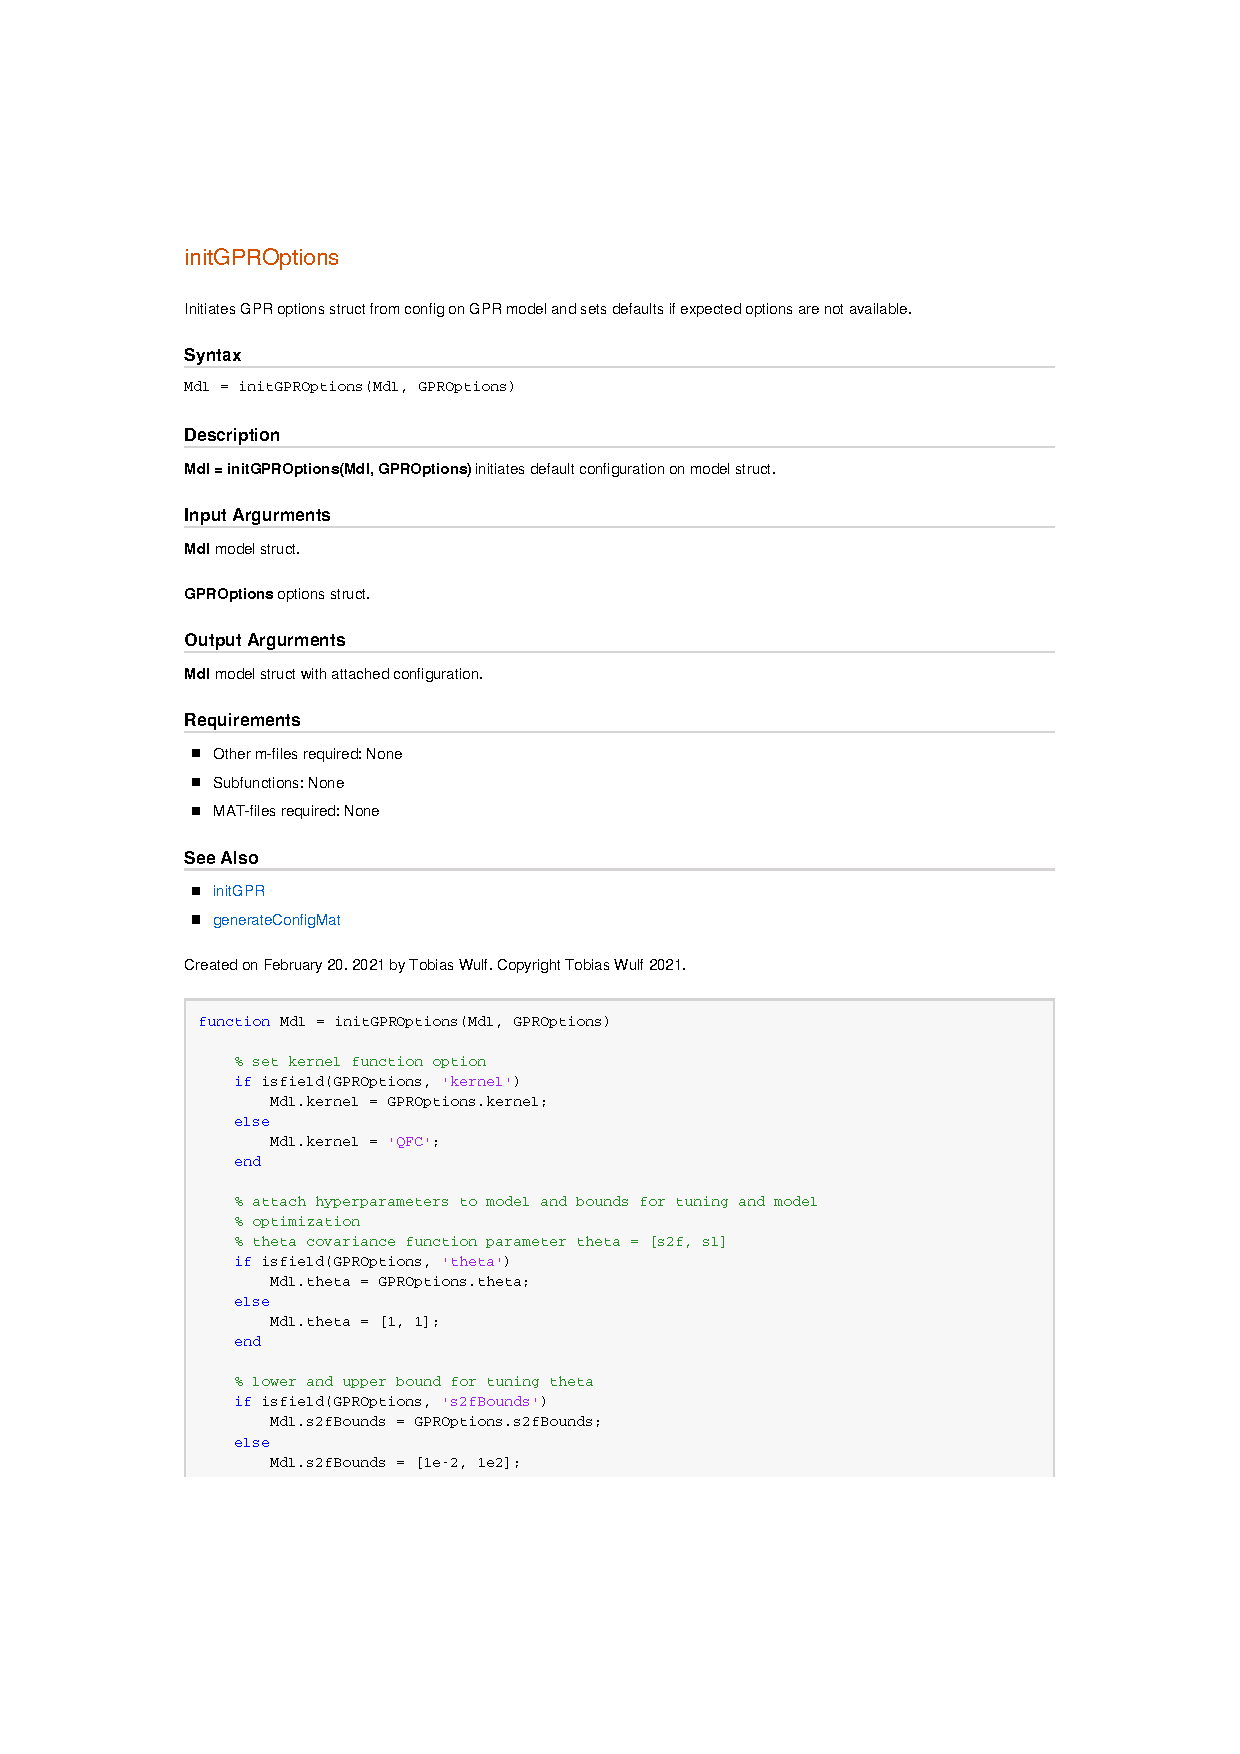
\includepdf[page=1,pagecommand={\phantomsection\addcontentsline{toc}{subsubsection}{\protect\numberline{\thesubsubsection}initGPROptions}\label{initGPROptions}}]{initGPROptions.pdf}
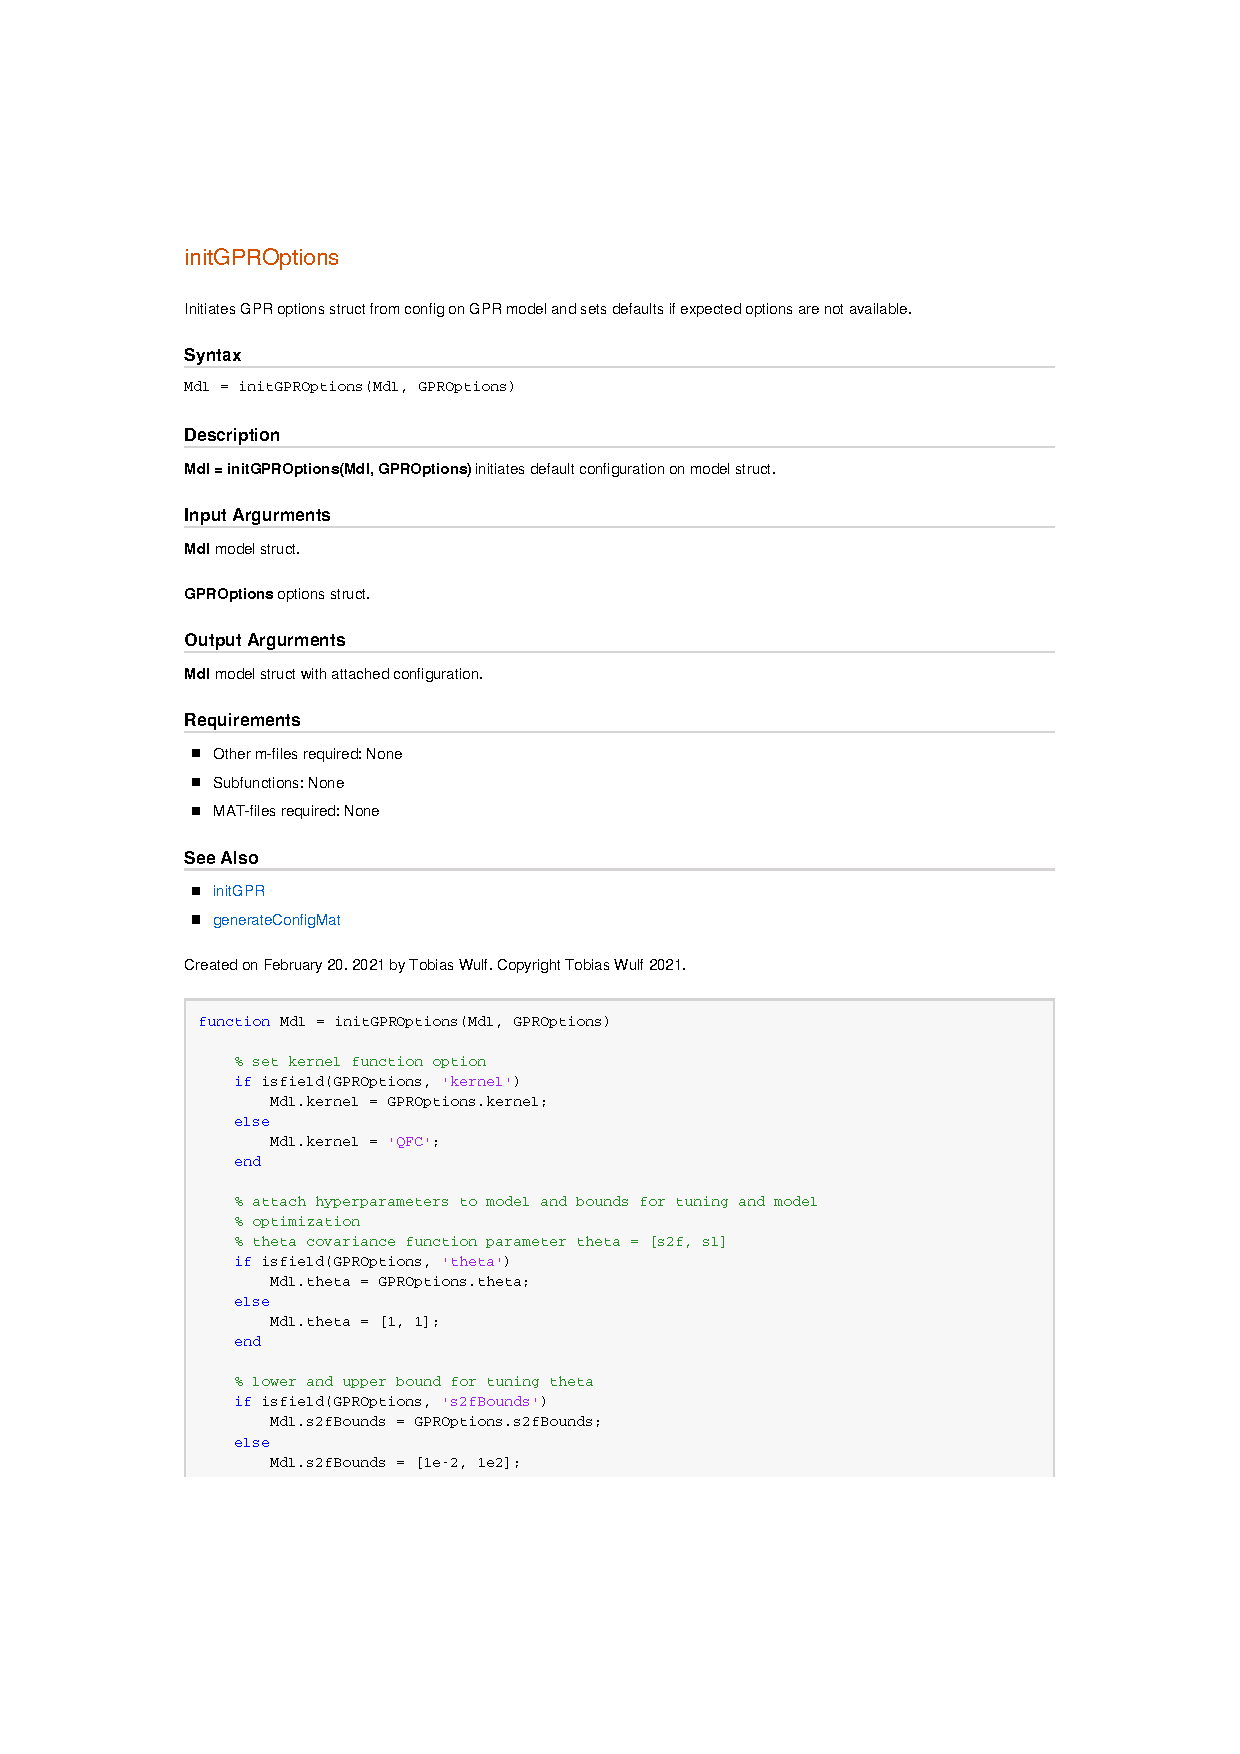
\includepdf[page=2-, pagecommand={\phantomsection}]{initGPROptions.pdf}
\addtocounter{subsubsection}{1}
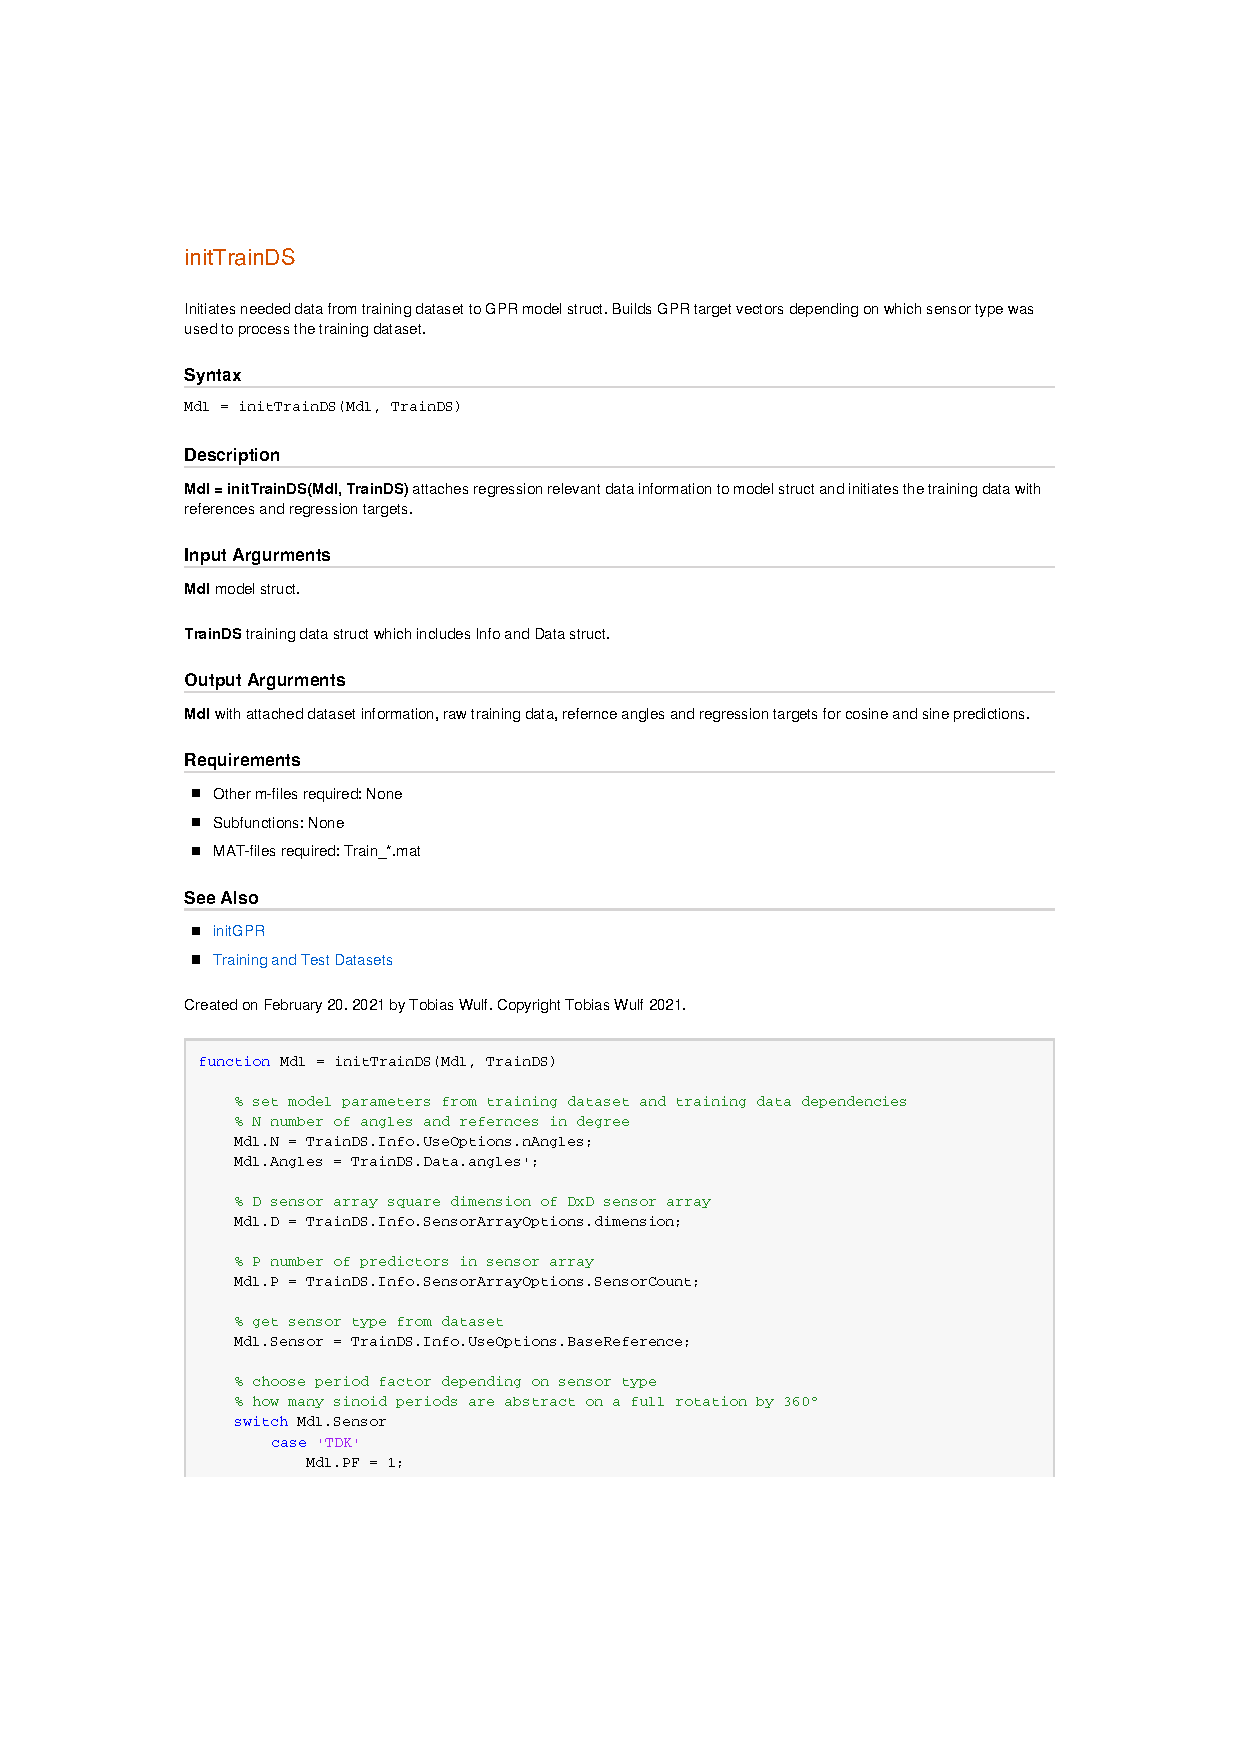
\includepdf[page=1,pagecommand={\phantomsection\addcontentsline{toc}{subsubsection}{\protect\numberline{\thesubsubsection}initTrainDS}\label{initTrainDS}}]{initTrainDS.pdf}
\includepdf[page=2-, pagecommand={\phantomsection}]{initTrainDS.pdf}
\addtocounter{subsubsection}{1}
\includepdf[page=1,pagecommand={\phantomsection\addcontentsline{toc}{subsubsection}{\protect\numberline{\thesubsubsection}initKernel}\label{initKernel}}]{initKernel.pdf}
\addtocounter{subsubsection}{1}
\includepdf[page=1,pagecommand={\phantomsection\addcontentsline{toc}{subsubsection}{\protect\numberline{\thesubsubsection}initKernelParameters}\label{initKernelParameters}}]{initKernelParameters.pdf}
\includepdf[page=2-, pagecommand={\phantomsection}]{initKernelParameters.pdf}
\addtocounter{subsubsection}{1}
\includepdf[page=1,pagecommand={\phantomsection\addcontentsline{toc}{subsubsection}{\protect\numberline{\thesubsubsection}tuneKernel}\label{tuneKernel}}]{tuneKernel.pdf}
\includepdf[page=2-, pagecommand={\phantomsection}]{tuneKernel.pdf}
\addtocounter{subsubsection}{1}
\includepdf[page=1,pagecommand={\phantomsection\addcontentsline{toc}{subsubsection}{\protect\numberline{\thesubsubsection}computeTuneCriteria}\label{computeTuneCriteria}}]{computeTuneCriteria.pdf}
\addtocounter{subsubsection}{1}
\includepdf[page=1,pagecommand={\phantomsection\addcontentsline{toc}{subsubsection}{\protect\numberline{\thesubsubsection}predFrame}\label{predFrame}}]{predFrame.pdf}
\includepdf[page=2-, pagecommand={\phantomsection}]{predFrame.pdf}
\addtocounter{subsubsection}{1}
\includepdf[page=1,pagecommand={\phantomsection\addcontentsline{toc}{subsubsection}{\protect\numberline{\thesubsubsection}predDS}\label{predDS}}]{predDS.pdf}
\includepdf[page=2-, pagecommand={\phantomsection}]{predDS.pdf}
\addtocounter{subsubsection}{1}
\includepdf[page=1,pagecommand={\phantomsection\addcontentsline{toc}{subsubsection}{\protect\numberline{\thesubsubsection}lossDS}\label{lossDS}}]{lossDS.pdf}
\includepdf[page=2-, pagecommand={\phantomsection}]{lossDS.pdf}
\addtocounter{subsubsection}{1}
\includepdf[page=1,pagecommand={\phantomsection\addcontentsline{toc}{subsubsection}{\protect\numberline{\thesubsubsection}optimGPR}\label{optimGPR}}]{optimGPR.pdf}
\includepdf[page=2-, pagecommand={\phantomsection}]{optimGPR.pdf}
\addtocounter{subsubsection}{1}
\includepdf[page=1,pagecommand={\phantomsection\addcontentsline{toc}{subsubsection}{\protect\numberline{\thesubsubsection}computeOptimCriteria}\label{computeOptimCriteria}}]{computeOptimCriteria.pdf}
\includepdf[page=2-, pagecommand={\phantomsection}]{computeOptimCriteria.pdf}
\addtocounter{subsubsection}{1}
\includepdf[page=1,pagecommand={\phantomsection\addcontentsline{toc}{subsubsection}{\protect\numberline{\thesubsubsection}kernelQFCAPX}\label{kernelQFCAPX}}]{kernelQFCAPX.pdf}
\addtocounter{paragraph}{1}
\includepdf[page=1,pagecommand={\phantomsection\addcontentsline{toc}{paragraph}{\protect\numberline{\theparagraph}QFCAPX}\label{QFCAPX}}]{QFCAPX.pdf}
\includepdf[page=2-, pagecommand={\phantomsection}]{QFCAPX.pdf}
\addtocounter{paragraph}{1}
\includepdf[page=1,pagecommand={\phantomsection\addcontentsline{toc}{paragraph}{\protect\numberline{\theparagraph}meanPolyQFCAPX}\label{meanPolyQFCAPX}}]{meanPolyQFCAPX.pdf}
\includepdf[page=2-, pagecommand={\phantomsection}]{meanPolyQFCAPX.pdf}
\addtocounter{paragraph}{1}
\includepdf[page=1,pagecommand={\phantomsection\addcontentsline{toc}{paragraph}{\protect\numberline{\theparagraph}initQFCAPX}\label{initQFCAPX}}]{initQFCAPX.pdf}
\includepdf[page=2-, pagecommand={\phantomsection}]{initQFCAPX.pdf}
\addtocounter{subsubsection}{1}
\includepdf[page=1,pagecommand={\phantomsection\addcontentsline{toc}{subsubsection}{\protect\numberline{\thesubsubsection}kernelQFC}\label{kernelQFC}}]{kernelQFC.pdf}
\addtocounter{paragraph}{1}
\includepdf[page=1,pagecommand={\phantomsection\addcontentsline{toc}{paragraph}{\protect\numberline{\theparagraph}QFC}\label{QFC}}]{QFC.pdf}
\includepdf[page=2-, pagecommand={\phantomsection}]{QFC.pdf}
\addtocounter{paragraph}{1}
\includepdf[page=1,pagecommand={\phantomsection\addcontentsline{toc}{paragraph}{\protect\numberline{\theparagraph}meanPolyQFC}\label{meanPolyQFC}}]{meanPolyQFC.pdf}
\includepdf[page=2-, pagecommand={\phantomsection}]{meanPolyQFC.pdf}
\addtocounter{paragraph}{1}
\includepdf[page=1,pagecommand={\phantomsection\addcontentsline{toc}{paragraph}{\protect\numberline{\theparagraph}initQFC}\label{initQFC}}]{initQFC.pdf}
\includepdf[page=2-, pagecommand={\phantomsection}]{initQFC.pdf}
\addtocounter{subsubsection}{1}
\includepdf[page=1,pagecommand={\phantomsection\addcontentsline{toc}{subsubsection}{\protect\numberline{\thesubsubsection}basicMathFunctions}\label{basicMathFunctions}}]{basicMathFunctions.pdf}
\addtocounter{paragraph}{1}
\includepdf[page=1,pagecommand={\phantomsection\addcontentsline{toc}{paragraph}{\protect\numberline{\theparagraph}sinoids2angles}\label{sinoids2angles}}]{sinoids2angles.pdf}
\includepdf[page=2-, pagecommand={\phantomsection}]{sinoids2angles.pdf}
\addtocounter{paragraph}{1}
\includepdf[page=1,pagecommand={\phantomsection\addcontentsline{toc}{paragraph}{\protect\numberline{\theparagraph}angles2sinoids}\label{angles2sinoids}}]{angles2sinoids.pdf}
\includepdf[page=2-, pagecommand={\phantomsection}]{angles2sinoids.pdf}
\addtocounter{paragraph}{1}
\includepdf[page=1,pagecommand={\phantomsection\addcontentsline{toc}{paragraph}{\protect\numberline{\theparagraph}decomposeChol}\label{decomposeChol}}]{decomposeChol.pdf}
\includepdf[page=2-, pagecommand={\phantomsection}]{decomposeChol.pdf}
\addtocounter{paragraph}{1}
\includepdf[page=1,pagecommand={\phantomsection\addcontentsline{toc}{paragraph}{\protect\numberline{\theparagraph}frobeniusNorm}\label{frobeniusNorm}}]{frobeniusNorm.pdf}
\includepdf[page=2-, pagecommand={\phantomsection}]{frobeniusNorm.pdf}
\addtocounter{paragraph}{1}
\includepdf[page=1,pagecommand={\phantomsection\addcontentsline{toc}{paragraph}{\protect\numberline{\theparagraph}computeInverseMatrixProduct}\label{computeInverseMatrixProduct}}]{computeInverseMatrixProduct.pdf}
\includepdf[page=2-, pagecommand={\phantomsection}]{computeInverseMatrixProduct.pdf}
\addtocounter{paragraph}{1}
\includepdf[page=1,pagecommand={\phantomsection\addcontentsline{toc}{paragraph}{\protect\numberline{\theparagraph}computeTransposeInverseProduct}\label{computeTransposeInverseProduct}}]{computeTransposeInverseProduct.pdf}
\includepdf[page=2-, pagecommand={\phantomsection}]{computeTransposeInverseProduct.pdf}
\addtocounter{paragraph}{1}
\includepdf[page=1,pagecommand={\phantomsection\addcontentsline{toc}{paragraph}{\protect\numberline{\theparagraph}addNoise2Covariance}\label{addNoise2Covariance}}]{addNoise2Covariance.pdf}
\includepdf[page=2-, pagecommand={\phantomsection}]{addNoise2Covariance.pdf}
\addtocounter{paragraph}{1}
\includepdf[page=1,pagecommand={\phantomsection\addcontentsline{toc}{paragraph}{\protect\numberline{\theparagraph}computeAlphaWeights}\label{computeAlphaWeights}}]{computeAlphaWeights.pdf}
\addtocounter{paragraph}{1}
\includepdf[page=1,pagecommand={\phantomsection\addcontentsline{toc}{paragraph}{\protect\numberline{\theparagraph}computeStdLogLoss}\label{computeStdLogLoss}}]{computeStdLogLoss.pdf}
\includepdf[page=2-, pagecommand={\phantomsection}]{computeStdLogLoss.pdf}
\addtocounter{paragraph}{1}
\includepdf[page=1,pagecommand={\phantomsection\addcontentsline{toc}{paragraph}{\protect\numberline{\theparagraph}computeLogLikelihood}\label{computeLogLikelihood}}]{computeLogLikelihood.pdf}
\includepdf[page=2-, pagecommand={\phantomsection}]{computeLogLikelihood.pdf}
\addtocounter{paragraph}{1}
\includepdf[page=1,pagecommand={\phantomsection\addcontentsline{toc}{paragraph}{\protect\numberline{\theparagraph}estimateBeta}\label{estimateBeta}}]{estimateBeta.pdf}
\includepdf[page=2-, pagecommand={\phantomsection}]{estimateBeta.pdf}
\addtocounter{subsection}{1}
\includepdf[page=1,pagecommand={\phantomsection\addcontentsline{toc}{subsection}{\protect\numberline{\thesubsection}util}\label{util}}]{util.pdf}
\addtocounter{subsubsection}{1}
\includepdf[page=1,pagecommand={\phantomsection\addcontentsline{toc}{subsubsection}{\protect\numberline{\thesubsubsection}removeFilesFromDir}\label{removeFilesFromDir}}]{removeFilesFromDir.pdf}
\includepdf[page=2-, pagecommand={\phantomsection}]{removeFilesFromDir.pdf}
\addtocounter{subsubsection}{1}
\includepdf[page=1,pagecommand={\phantomsection\addcontentsline{toc}{subsubsection}{\protect\numberline{\thesubsubsection}publishFilesFromDir}\label{publishFilesFromDir}}]{publishFilesFromDir.pdf}
\includepdf[page=2-, pagecommand={\phantomsection}]{publishFilesFromDir.pdf}
\addtocounter{subsubsection}{1}
\includepdf[page=1,pagecommand={\phantomsection\addcontentsline{toc}{subsubsection}{\protect\numberline{\thesubsubsection}plotFunctions}\label{plotFunctions}}]{plotFunctions.pdf}
\includepdf[page=2-, pagecommand={\phantomsection}]{plotFunctions.pdf}
\addtocounter{paragraph}{1}
\includepdf[page=1,pagecommand={\phantomsection\addcontentsline{toc}{paragraph}{\protect\numberline{\theparagraph}plotTDKCharDataset}\label{plotTDKCharDataset}}]{plotTDKCharDataset.pdf}
\includepdf[page=2-, pagecommand={\phantomsection}]{plotTDKCharDataset.pdf}
\addtocounter{paragraph}{1}
\includepdf[page=1,pagecommand={\phantomsection\addcontentsline{toc}{paragraph}{\protect\numberline{\theparagraph}plotTDKCharField}\label{plotTDKCharField}}]{plotTDKCharField.pdf}
\includepdf[page=2-, pagecommand={\phantomsection}]{plotTDKCharField.pdf}
\addtocounter{paragraph}{1}
\includepdf[page=1,pagecommand={\phantomsection\addcontentsline{toc}{paragraph}{\protect\numberline{\theparagraph}plotTDKTransferCurves}\label{plotTDKTransferCurves}}]{plotTDKTransferCurves.pdf}
\includepdf[page=2-, pagecommand={\phantomsection}]{plotTDKTransferCurves.pdf}
\addtocounter{paragraph}{1}
\includepdf[page=1,pagecommand={\phantomsection\addcontentsline{toc}{paragraph}{\protect\numberline{\theparagraph}plotKMZ60CharDataset}\label{plotKMZ60CharDataset}}]{plotKMZ60CharDataset.pdf}
\includepdf[page=2-, pagecommand={\phantomsection}]{plotKMZ60CharDataset.pdf}
\addtocounter{paragraph}{1}
\includepdf[page=1,pagecommand={\phantomsection\addcontentsline{toc}{paragraph}{\protect\numberline{\theparagraph}plotKMZ60CharField}\label{plotKMZ60CharField}}]{plotKMZ60CharField.pdf}
\includepdf[page=2-, pagecommand={\phantomsection}]{plotKMZ60CharField.pdf}
\addtocounter{paragraph}{1}
\includepdf[page=1,pagecommand={\phantomsection\addcontentsline{toc}{paragraph}{\protect\numberline{\theparagraph}plotKMZ60TransferCurves}\label{plotKMZ60TransferCurves}}]{plotKMZ60TransferCurves.pdf}
\includepdf[page=2-, pagecommand={\phantomsection}]{plotKMZ60TransferCurves.pdf}
\addtocounter{paragraph}{1}
\includepdf[page=1,pagecommand={\phantomsection\addcontentsline{toc}{paragraph}{\protect\numberline{\theparagraph}plotDipoleMagnet}\label{plotDipoleMagnet}}]{plotDipoleMagnet.pdf}
\includepdf[page=2-, pagecommand={\phantomsection}]{plotDipoleMagnet.pdf}
\addtocounter{paragraph}{1}
\includepdf[page=1,pagecommand={\phantomsection\addcontentsline{toc}{paragraph}{\protect\numberline{\theparagraph}plotSimulationDataset}\label{plotSimulationDataset}}]{plotSimulationDataset.pdf}
\includepdf[page=2-, pagecommand={\phantomsection}]{plotSimulationDataset.pdf}
\addtocounter{paragraph}{1}
\includepdf[page=1,pagecommand={\phantomsection\addcontentsline{toc}{paragraph}{\protect\numberline{\theparagraph}plotSingleSimulationAngle}\label{plotSingleSimulationAngle}}]{plotSingleSimulationAngle.pdf}
\includepdf[page=2-, pagecommand={\phantomsection}]{plotSingleSimulationAngle.pdf}
\addtocounter{paragraph}{1}
\includepdf[page=1,pagecommand={\phantomsection\addcontentsline{toc}{paragraph}{\protect\numberline{\theparagraph}plotSimulationSubset}\label{plotSimulationSubset}}]{plotSimulationSubset.pdf}
\includepdf[page=2-, pagecommand={\phantomsection}]{plotSimulationSubset.pdf}
\addtocounter{paragraph}{1}
\includepdf[page=1,pagecommand={\phantomsection\addcontentsline{toc}{paragraph}{\protect\numberline{\theparagraph}plotSimulationCosSinStats}\label{plotSimulationCosSinStats}}]{plotSimulationCosSinStats.pdf}
\includepdf[page=2-, pagecommand={\phantomsection}]{plotSimulationCosSinStats.pdf}
\addtocounter{paragraph}{1}
\includepdf[page=1,pagecommand={\phantomsection\addcontentsline{toc}{paragraph}{\protect\numberline{\theparagraph}plotSimulationDatasetCircle}\label{plotSimulationDatasetCircle}}]{plotSimulationDatasetCircle.pdf}
\includepdf[page=2-, pagecommand={\phantomsection}]{plotSimulationDatasetCircle.pdf}
\addtocounter{section}{1}
\includepdf[page=1,pagecommand={\phantomsection\addcontentsline{toc}{section}{\protect\numberline{\thesection}Datasets}\label{Datasets}}]{Datasets.pdf}
\addtocounter{subsection}{1}
\includepdf[page=1,pagecommand={\phantomsection\addcontentsline{toc}{subsection}{\protect\numberline{\thesubsection}TDK TAS2141 Characterization}\label{TDK TAS2141 Characterization}}]{TDK_TAS2141_Characterization.pdf}
\includepdf[page=2-, pagecommand={\phantomsection}]{TDK_TAS2141_Characterization.pdf}
\addtocounter{subsection}{1}
\includepdf[page=1,pagecommand={\phantomsection\addcontentsline{toc}{subsection}{\protect\numberline{\thesubsection}NXP KMZ60 Characterization}\label{NXP KMZ60 Characterization}}]{NXP_KMZ60_Characterization.pdf}
\includepdf[page=2-, pagecommand={\phantomsection}]{NXP_KMZ60_Characterization.pdf}
\addtocounter{subsection}{1}
\includepdf[page=1,pagecommand={\phantomsection\addcontentsline{toc}{subsection}{\protect\numberline{\thesubsection}Config Mat}\label{Config Mat}}]{Config_Mat.pdf}
\addtocounter{subsection}{1}
\includepdf[page=1,pagecommand={\phantomsection\addcontentsline{toc}{subsection}{\protect\numberline{\thesubsection}Training and Test Datasets}\label{Training and Test Datasets}}]{Training_and_Test_Datasets.pdf}
\includepdf[page=2-, pagecommand={\phantomsection}]{Training_and_Test_Datasets.pdf}
\addtocounter{section}{1}
\includepdf[page=1,pagecommand={\phantomsection\addcontentsline{toc}{section}{\protect\numberline{\thesection}Unit Tests}\label{Unit Tests}}]{Unit_Tests.pdf}
\includepdf[page=2-, pagecommand={\phantomsection}]{Unit_Tests.pdf}
\addtocounter{subsection}{1}
\includepdf[page=1,pagecommand={\phantomsection\addcontentsline{toc}{subsection}{\protect\numberline{\thesubsection}runTests}\label{runTests}}]{runTests.pdf}
\addtocounter{subsection}{1}
\includepdf[page=1,pagecommand={\phantomsection\addcontentsline{toc}{subsection}{\protect\numberline{\thesubsection}removeFilesFromDirTest}\label{removeFilesFromDirTest}}]{removeFilesFromDirTest.pdf}
\addtocounter{subsection}{1}
\includepdf[page=1,pagecommand={\phantomsection\addcontentsline{toc}{subsection}{\protect\numberline{\thesubsection}rotate3DVectorTest}\label{rotate3DVectorTest}}]{rotate3DVectorTest.pdf}
\includepdf[page=2-, pagecommand={\phantomsection}]{rotate3DVectorTest.pdf}
\addtocounter{subsection}{1}
\includepdf[page=1,pagecommand={\phantomsection\addcontentsline{toc}{subsection}{\protect\numberline{\thesubsection}generateDipoleRotationMomentsTest}\label{generateDipoleRotationMomentsTest}}]{generateDipoleRotationMomentsTest.pdf}
\addtocounter{subsection}{1}
\includepdf[page=1,pagecommand={\phantomsection\addcontentsline{toc}{subsection}{\protect\numberline{\thesubsection}generateSensorArraySquareGridTest}\label{generateSensorArraySquareGridTest}}]{generateSensorArraySquareGridTest.pdf}
\addtocounter{subsection}{1}
\includepdf[page=1,pagecommand={\phantomsection\addcontentsline{toc}{subsection}{\protect\numberline{\thesubsection}computeDipoleH0NormTest}\label{computeDipoleH0NormTest}}]{computeDipoleH0NormTest.pdf}
\addtocounter{subsection}{1}
\includepdf[page=1,pagecommand={\phantomsection\addcontentsline{toc}{subsection}{\protect\numberline{\thesubsection}computeDipoleHFieldTest}\label{computeDipoleHFieldTest}}]{computeDipoleHFieldTest.pdf}
\includepdf[page=2-, pagecommand={\phantomsection}]{computeDipoleHFieldTest.pdf}
\addtocounter{subsection}{1}
\includepdf[page=1,pagecommand={\phantomsection\addcontentsline{toc}{subsection}{\protect\numberline{\thesubsection}tiltRotationTest}\label{tiltRotationTest}}]{tiltRotationTest.pdf}
\includepdf[page=2-, pagecommand={\phantomsection}]{tiltRotationTest.pdf}
